%%%%%%%%%%%%%%%%%%%%%%%%%%%%%%%%%%%%%%%%%
% Tufte-Style Book (Minimal Template)
% LaTeX Template
% Version 1.0 (5/1/13)
%
% This template has been downloaded from:
% http://www.LaTeXTemplates.com
%
% License:
% CC BY-NC-SA 3.0 (http://creativecommons.org/licenses/by-nc-sa/3.0/)
%
% IMPORTANT NOTE:
% In addition to running BibTeX to compile the reference list from the .bib
% file, you will need to run MakeIndex to compile the index at the end of the
% document.
%
%%%%%%%%%%%%%%%%%%%%%%%%%%%%%%%%%%%%%%%%%

%----------------------------------------------------------------------------------------
%	PACKAGES AND OTHER DOCUMENT CONFIGURATIONS
%----------------------------------------------------------------------------------------

\documentclass{tufte-book} % Use the tufte-book class which in turn uses the tufte-common class

\usepackage{natbib}

\hypersetup{colorlinks} % Comment this line if you don't wish to have colored links

\usepackage{microtype} % Improves character and word spacing

%\usepackage{lipsum} % Inserts dummy text

\usepackage{booktabs} % Better horizontal rules in tables

\usepackage{graphicx} % Needed to insert images into the document
\graphicspath{{graphics/}} % Sets the default location of pictures
\setkeys{Gin}{width=\linewidth,totalheight=\textheight,keepaspectratio} % Improves figure scaling

\usepackage{fancyvrb} % Allows customization of verbatim environments
\fvset{fontsize=\normalsize} % The font size of all verbatim text can be changed here

\newcommand{\hangp}[1]{\makebox[0pt][r]{(}#1\makebox[0pt][l]{)}} % New command to create parentheses around text in tables which take up no horizontal space - this improves column spacing
\newcommand{\hangstar}{\makebox[0pt][l]{*}} % New command to create asterisks in tables which take up no horizontal space - this improves column spacing

\usepackage{xspace} % Used for printing a trailing space better than using a tilde (~) using the \xspace command

\newcommand{\monthyear}{\ifcase\month\or January\or February\or March\or April\or May\or June\or July\or August\or September\or October\or November\or December\fi\space\number\year} % A command to print the current month and year

\newcommand{\openepigraph}[2]{ % This block sets up a command for printing an epigraph with 2 arguments - the quote and the author
\begin{fullwidth}
\sffamily\large
\begin{doublespace}
\noindent\allcaps{#1}\\ % The quote
\noindent\allcaps{#2} % The author
\end{doublespace}
\end{fullwidth}
}

\newcommand{\blankpage}{\newpage\hbox{}\thispagestyle{empty}\newpage} % Command to insert a blank page

\usepackage{makeidx} % Used to generate the index
\makeindex % Generate the index which is printed at the end of the document

%----------------------------------------------------------------------------------------
%	BOOK META-INFORMATION
%----------------------------------------------------------------------------------------

\title{Notes on\\Star Formation} % Title of the book

\author{Mark R.~Krumholz} % Author

\publisher{The Open Astrophysics Bookshelf} % Publisher

%----------------------------------------------------------------------------------------

%----------------------------------------------------------------------------------------
% MRK customizations

% Symbols used throughout
% Local symbols
\newcommand{\kb}{k_{\mathrm{B}}}
\newcommand{\msun}{M_{\odot}}
\newcommand{\rsun}{R_{\odot}}
\newcommand{\lsun}{L_{\odot}}
\newcommand{\vecr}{\mathbf{r}}
\newcommand{\vecv}{\mathbf{v}}
\newcommand{\vecx}{\mathbf{x}}
\newcommand{\veck}{\mathbf{k}}
\newcommand{\vecB}{\mathbf{B}}
\newcommand{\vecf}{\mathbf{f}}
\newcommand{\nhat}{\hat{\mathbf{n}}}
\newcommand{\vecS}{\mathbf{S}}
\newcommand{\vecI}{\mathbf{I}}
\newcommand{\vecPi}{\mathbf{\Pi}}
\newcommand{\vecT}{\mathbf{T}}

% AAStex symbols
\usepackage{amssymb}

% Journals
\newcommand{\aap}{Astron.~\& Astrophys.}
\newcommand{\apj}{Astrophys.~J.}
\newcommand{\apjs}{Astrophys.~J.~Supp.}
\newcommand{\apjl}{Astrophys.~J.}
\newcommand{\aj}{Astron.~J.}
\newcommand{\araa}{Annu.~Rev.~Astron.~Astrophys.}
\newcommand{\pasp}{Proc.~Astron.~Soc.~Pac.}
\newcommand{\mnras}{Mon.~Not.~Roy.~Astron.~Soc.}


% Autoref for marginfigures
%\newcommand{\marginfigureautorefname}{Figure}

% Journals
\newcommand{\aap}{Astron.~\& Astrophys.}
\newcommand{\apj}{Astrophys.~J.}
\newcommand{\aj}{Astron.~J.}
\newcommand{\araa}{Annu.~Rev.~Astron.~Astrophys.}
\newcommand{\pasp}{Proc.~Astron.~Soc.~Pac.}
\newcommand{\mnras}{Mon.~Not.~Roy.~Astron.~Soc.}

%----------------------------------------------------------------------------------------

\begin{document}

\frontmatter

%----------------------------------------------------------------------------------------
%	EPIGRAPH
%----------------------------------------------------------------------------------------

\thispagestyle{empty}
%\openepigraph{Quotation 1}{Author, {\itshape Source}}
%\vfill
%\openepigraph{Quotation 2}{Author}
%\vfill
%\openepigraph{Quotation 3}{Author}

%----------------------------------------------------------------------------------------

\maketitle % Print the title page

%----------------------------------------------------------------------------------------
%	COPYRIGHT PAGE
%----------------------------------------------------------------------------------------

\newpage
\begin{fullwidth}
~\vfill
\thispagestyle{empty}
\setlength{\parindent}{0pt}
\setlength{\parskip}{\baselineskip}
Original version: \the\year\ \thanklessauthor

\par\smallcaps{Published as part of the Open Astrophysics Bookshelf}

\par\smallcaps{\url{http://open-astrophysics-bookshelf.github.io/}}

\par Licensed under the Creative Commons 1.0 Universal License, \url{http://creativecommons.org/publicdomain/zero/1.0/}.\index{license}

%\par\textit{First printing, \monthyear}
\end{fullwidth}

%----------------------------------------------------------------------------------------

\tableofcontents % Print the table of contents

%----------------------------------------------------------------------------------------

\listoffigures % Print a list of figures

%----------------------------------------------------------------------------------------

\listoftables % Print a list of tables

%----------------------------------------------------------------------------------------
%	DEDICATION PAGE
%----------------------------------------------------------------------------------------

%\cleardoublepage
%~\vfill
%\begin{doublespace}
%\noindent\fontsize{18}{22}\selectfont\itshape
%\nohyphenation
%Dedicated to my family and friends.
%\end{doublespace}
%\vfill
%\vfill

%----------------------------------------------------------------------------------------
%	INTRODUCTION
%----------------------------------------------------------------------------------------

\cleardoublepage
\chapter*{Introduction} % The asterisk leaves out this chapter from the table of contents

This book is based on a series of lectures given by the author in his graduate class on star formation, taught from 2009 - 2014 at UC Santa Cruz. It is intended for graduate students or advanced undergraduates in astronomy or physics, but does not presume detailed knowledge of particular areas of astrophysics (e.g., the interstellar medium or galactic structure). It is intended to provide a general overview of the field of star formation, at a level that would enable a student to begin independent research in the area.

This course covers the basics of star formation and ending at the transition to planet formation. The structure of the course / book is as follows. Each chapter corresponds roughly to a single lecture. The first two chapters begin with a discussion of observational techniques, and the basic phenomenology they reveal. The goal is to familiarize students with the basic techniques that will be used throughout, and to provide a common vocabulary for the rest of the course. The next four chapters provide a similar review of the basic physical processes that are important for star formation. Again, the goal is to provide a basis for what follows. The remaining chapters discuss star formation over a variety of scales, starting with the galactic scale and working our way down to the scales of individual stars and their disks. The course concludes with the clearing of disks and the transition to planet formation.

The "text" intended to go with these notes is the review article "\href{http://adsabs.harvard.edu/abs/2014arXiv1402.0867K}{The Big Problems in Star Formation: the Star Formation Rate, Stellar Clustering, and the Initial Mass Function}", Krumholz, M. R., 2014, \textit{Physics Reports}, 539, 49, which provides a snapshot of the literature as of the most recent time the course was given. Another extremely useful reference is the series of review chapters from the \href{http://www.mpia.de/homes/ppvi/}{Protostars and Planets VI Conference}, which took place in July 2013.

In addition to the text, this book contains five problem sets, which are interspersed with the chapters at appropriate locations. Solutions to the problems are included at the end.

%Citation example \cite{Tufte2001}, notice how the citation is in the margin. This is an example of how to add something to the index at the end of the document.\index{citation}

%\newthought{Example of} the \texttt{newthought} command for starting new sections. Typography examples: \allcaps{all caps} and \smallcaps{small caps}.

%------------------------------------------------

%\section{Figures}

%\lipsum[1] 

%\begin{marginfigure}
%\includegraphics[width=\linewidth]{helix}
%\caption{This is a margin figure. The helix is defined by $x = \cos(2\pi z)$, $y = \sin(2\pi z)$, and $z = [0, 2.7]$. The figure was drawn using Asymptote (\url{http://asymptote.sf.net/}).}
%\label{fig:marginfig}
%\end{marginfigure}

%\lipsum[2]

%\begin{figure*}[h]
%\includegraphics[width=\linewidth]{sine.pdf}
%\caption{This graph shows $y = \sin x$ from about $x = [-10, 10]$.
%\emph{Notice that this figure takes up the full page width.}}
%\label{fig:fullfig}
%\end{figure*}

%\lipsum[3]

%------------------------------------------------

%\section{Tables} \marginnote{This is a random margin note. Notice that there isn't a number preceding the note, and there is no number in the main text where this note was written. Use \texttt{sidenote} to use a number.}

%\lipsum[4]

%\begin{table} % Add the following just after the closing bracket on this line to specify a position for the table on the page: [h], [t], [b] or [p] - these mean: here, top, bottom and on a separate page, respectively
%\centering % Centers the table on the page, comment out to left-justify
%\begin{tabular}{l c c c c c} % The final bracket specifies the number of columns in the table along with left and right borders which are specified using vertical bars (|); each column can be left, right or center-justified using l, r or c. To specify a precise width, use p{width}, e.g. p{5cm}
%\toprule % Top horizontal line
%& \multicolumn{5}{c}{Growth Media} \\ % Amalgamating several columns into one cell is done using the \multicolumn command as seen on this line
%\cmidrule(l){2-6} % Horizontal line spanning less than the full width of the table - you can add (r) or (l) just before the opening curly bracket to shorten the rule on the left or right side
%Strain & 1 & 2 & 3 & 4 & 5\\ % Column names row
%\midrule % In-table horizontal line
%GDS1002 & 0.962 & 0.821 & 0.356 & 0.682 & 0.801\\ % Content row 1
%NWN652 & 0.981 & 0.891 & 0.527 & 0.574 & 0.984\\ % Content row 2
%PPD234 & 0.915 & 0.936 & 0.491 & 0.276 & 0.965\\ % Content row 3
%JSB126 & 0.828 & 0.827 & 0.528 & 0.518 & 0.926\\ % Content row 4
%JSB724 & 0.916 & 0.933 & 0.482 & 0.644 & 0.937\\ % Content row 5
%\midrule % In-table horizontal line
%\midrule % In-table horizontal line
%Average Rate & 0.920 & 0.882 & 0.477 & 0.539 & 0.923\\ % Summary/total row
%\bottomrule % Bottom horizontal line
%\end{tabular}
%\caption{Table caption text} % Table caption, can be commented out if no caption is required
%\label{tab:template} % A label for referencing this table elsewhere, references are used in text as \ref{label}
%\end{table}

%----------------------------------------------------------------------------------------

% Number things
\setcounter{secnumdepth}{3}

\mainmatter

%----------------------------------------------------------------------------------------
%	CHAPTERS
%----------------------------------------------------------------------------------------

%\chapter{Chapter 1 Title}
%\label{ch:1}
\part{Introduction and Phenomenology}

\chapter{Observing the Cold Interstellar Medium}
\label{ch:obscold}

\marginnote{\textbf{Suggested background reading:}
\begin{itemize}
\item \href{http://adsabs.harvard.edu/abs/2012ARA\%26A..50..531K}{Kennicutt, R.~C., \& Evans, N.~J. 2012, ARA\&A, 50, 531}, sections $1-2$ \nocite{kennicutt12a}
\end{itemize}
}

This first chapter focuses on observations of interstellar gas. Because the interstellar clouds that form stars are generally cold, most (but not all) of these techniques require in infrared, sub-millimeter, and radio observations. Interpretation of the results is often highly non-trivial. This will naturally lead us to review some of the important radiative transfer physics that we need to keep in mind to understand the observations. With this background complete, we will then discuss the phenomenology of interstellar gas derived from these observations.

\section{Observing Techniques}

\subsection{The Problem of H$_2$}

\begin{marginfigure}
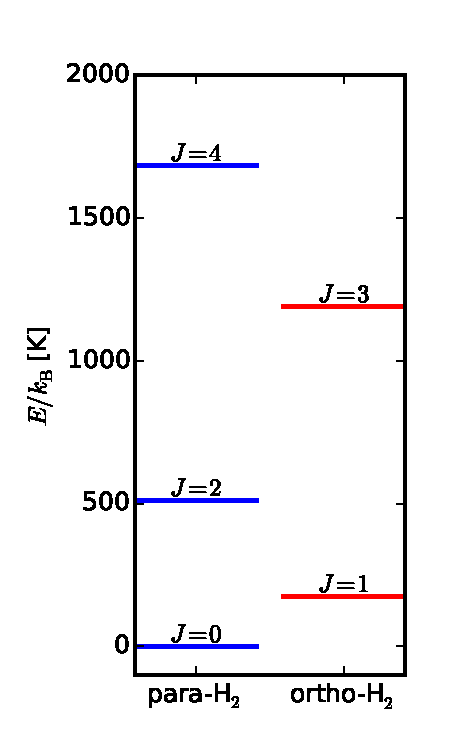
\includegraphics[width=\linewidth]{h2levels}
\caption[H$_2$ level diagram]{
\label{fig:h2levels}
Level diagram for the rotational levels of para- and ortho-H$_2$, showing the energy of each level. Level data are taken from \url{http://www.gemini.edu/sciops/instruments/nir/wavecal/h2lines.dat}.
}
\end{marginfigure}

Before we dive into all the tricks we use to observe the dense interstellar medium (ISM), we have to start at the question of why it is necessary to be so clever. Hydrogen is the most abundant element, and when it is in the form of free atomic hydrogen, it is relatively easy to observe. Hydrogen atoms emit radio waves at a wavelength of 21 cm (1.4 GHz), associated with a hyperfine transition from a state in which the spin of the electron is parallel to that of the proton to a state where it is anti-parallel. The energy difference between these two states corresponds to a temperature $\ll 1$ K, so even in cold regions it can be excited. This line is seen in the Milky Way and in many nearby galaxies.
  
However, at the high densities where stars form, hydrogen tends to be molecular rather than atomic, and H$_2$ is extremely hard to observe directly. To understand why, we can look at an energy level diagram for rotational levels of H$_2$ (Figure \ref{fig:h2levels}). A diatomic molecule like H$_2$ has three types of excitation: electronic (corresponding to excitations of one or more of the electrons), vibrational (corresponding to vibrational motion of the two nuclei), and rotational (corresponding to rotation of the two nuclei about the center of mass). Generally electronic excitations are highest in energy scale, vibrational are next, and rotational are the lowest in energy. Thus the levels shown in Figure \ref{fig:h2levels} are the ones that lie closest to ground.

For H$_2$, the first thing to notice is that the first excited state, the $J=1$ rotational state, is $175$ K above the ground state. Since the dense ISM where molecules form is often also cold, $T\sim 10$ K (as we will see later), almost no molecules will be in this excited state. However, it gets even worse: H$_2$ is a homonuclear molecule, and for reasons of symmetry $\Delta J = 1$ radiative transitions are forbidden in homonuclear molecules. Indeed, there is no electronic process by which a hydrogen molecule with odd $J$ to turn into one with even $J$, and vice versa, because the allowed parity of $J$ is determined by the spins of the hydrogen nuclei. We refer to the even $J$ state as para-H$_2$, and the odd $J$ state as ortho-H$_2$.

The observational significance of this is that there is no $J=1\rightarrow 0$ emission. Instead, the lowest-lying transition is the $J=2\rightarrow 0$ quadrupole. This is very weak, because it's a quadrupole. More importantly, however, the $J=2$ state is 510 K above the ground state. This means that, for a population in equilibrium at a temperature of 10 K, the fraction of molecules in the $J=2$ state is $\sim e^{-510/10} \approx 10^{-22}$!\footnote{This oversimplifies things quite a bit, because in real molecular clouds there are usually shocked regions where the temperature is much greater than 10 K, and H$_2$ rotational emission is routinely observed from them. However, this emission tracers rare gas that is much hotter than the mean temperature in a cloud, not the bulk of the mass, which is cold.} In effect, in a molecular cloud there are simply no H$_2$ molecules in states capable of emitting. The reason such a high temperature is required to excite the H$_2$ molecule is its low mass: for a quantum oscillator or rotor, the level spacing varies with reduced mass as $m^{-1/2}$. Thus the levels of H$_2$ are much farther apart than the levels of other diatomic molecules (e.g., CO, O$_2$, N$_2$). It is the low mass of the hydrogen atom that creates our problems.
  
Given this result, we see that, for the most part, observations of the most abundant species can only be done by proxy. Only in very rare circumstances is it possible to observe H$_2$ directly -- usually when there is a bright background UV source that allows us to see it in UV absorption rather than in emission. Since these circumstances do not generally prevail, we are forced to consider alternatives.

\subsection{Dust Emission}

The most conceptually straightforward proxy technique we use to study star-forming clouds is thermal dust emission. Interstellar gas clouds are always mixed with dust, and the dust grains emit thermal radiation that we can observe. The gas, in contrast, does not emit thermal radiation because it is nowhere near dense enough to reach equilibrium with the radiation field. Instead, gas emission comes primarily in the form of lines, which we will discuss below.
  
Consider a cloud of gas of mass density $\rho$ mixed with dust grains at a temperature $T$. The gas-dust mixture has an absorption opacity $\kappa_{\nu}$ to radiation at frequency $\nu$. Although the vast majority of the mass is in gas rather than dust, the opacity will be almost entirely due to the dust grains except for frequencies that happen to match the resonant absorption frequencies of atoms and molecules in the gas. Here we follow the standard astronomy convention that $\kappa_{\nu}$ is the opacity per gram of material, with units of cm$^2$ g$^{-1}$, i.e., we assign the gas an effective cross-sectional area that is blocked per gram of gas. For submillimeter observations, typical values of $\kappa_{\nu}$ are $\sim 0.01$ cm$^{2}$ g$^{-1}$. Figure \ref{fig:draine03opacity} shows a typical extinction curve for Milky Way dust.

\begin{marginfigure}
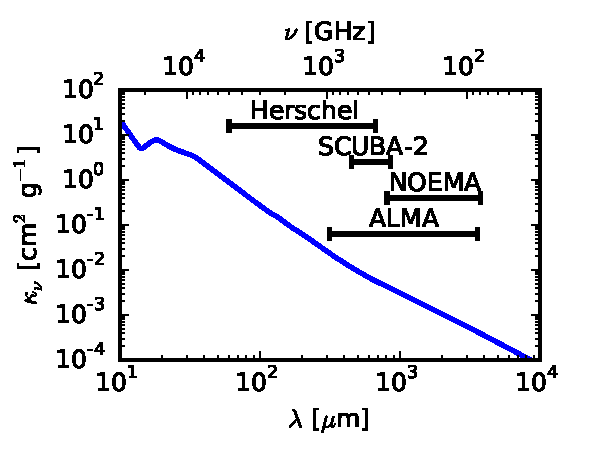
\includegraphics[width=\linewidth]{draine03opacity}
\caption[Dust absorption opacity]{
\label{fig:draine03opacity}
Milky Way dust absorption opacities per unit gas mass as a function of wavelength $\lambda$ and frequency $\nu$ in the infrared and sub-mm range, together with wavelength coverage of selected observational facilities. Dust opacities are taken from the model of \citet{draine03a} for $R_V = 5.5$.
}
\end{marginfigure}

Since essentially no interstellar cloud has a surface density $> 100$ g cm$^{-2}$, absorption of radiation from the back of the cloud by gas in front of it is completely negligible. Thus, we can compute the emitted intensity very easily. The emissivity for gas of opacity $\kappa_{\nu}$ is $j_{\nu} = \kappa_{\nu} \rho B_{\nu}(T)$, where $j_{\nu}$ has units of erg s$^{-1}$ cm$^{-3}$ sr$^{-1}$ Hz$^{-1}$, i.e.\ it describes (in cgs units) the number of ergs emitted in 1 second by 1 cm$^3$ of gas into a solid angle of 1 sr in a frequency range of 1 Hz. The quantity
\begin{equation}
B_{\nu}(T) = \frac{2 h\nu^3}{c^2} \frac{1}{e^{h\nu/\kb T}-1}
\end{equation}
is the Planck function.
  
Since none of this radiation is absorbed, we can compute the intensity transmitted along a given ray just by integrating the emission: 
  \begin{equation}
  I_{\nu} = \int j_{\nu} ds = \Sigma \kappa_{\nu} B_{\nu}(T) = \tau_{\nu} B_{\nu}(T)
  \end{equation}
where $\Sigma=\int \rho ds$ is the surface density of the cloud and $\tau_{\nu} = \Sigma \kappa_{\nu}$ is the optical depth of the cloud at frequency $\nu$. Thus if we observe the intensity of emission from dust grains in a cloud, we determine the product of the optical depth and the Planck function, which is determined solely by the observing frequency and the gas temperature. If we know the temperature and the properties of the dust grains, we can therefore determine the column density of the gas in the cloud in each telescope beam.

\begin{figure}
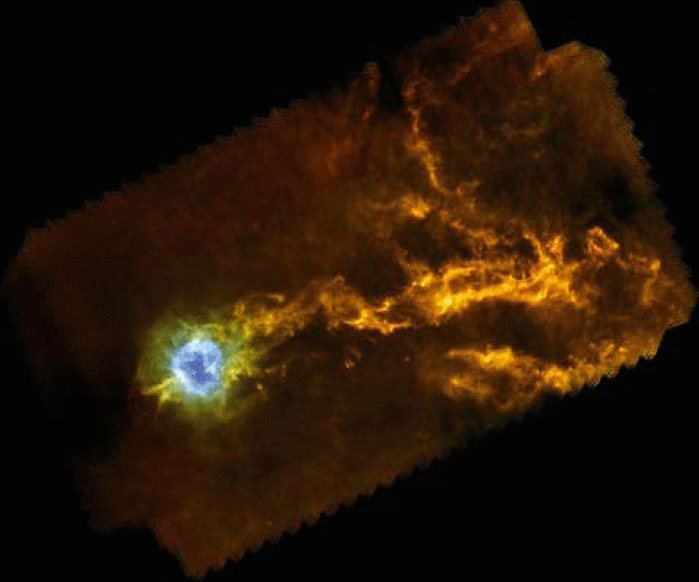
\includegraphics[width=\linewidth]{herschel_ic5146}
\caption[\textit{Herschel} map of IC 5146]{
\label{fig:herschel_ic5146}
Three-color composite image of IC 5146 taken by the SPIRE and PACS instruments aboard \textit{Herschel}. Red is SPIRE 500 $\mu$m, green is SPIRE 250 $\mu$m plus PACS 160 $\mu$m, and blue is PACS 70 $\mu$m. Credit: \citeauthor{arzoumanian11a}, A\&A, 529, L6, 2011, reproduced with permission \copyright\,ESO.
}
\end{figure}

Figure \ref{fig:herschel_ic5146} show an example result using this technique. The advantage of this approach is that it is very straightforward. The major uncertainties are in the dust opacity, which we probably don't know better than a factor of few level, and in the gas temperature, which is also usually uncertain at the factor of $\sim 2$ level. The produces a corresponding uncertainty in the conversion between dust emission and gas column density. Both of these can be improved substantially by observations that cover a wide variety of wavelengths, since these allow one to simultaneously fit the column density, dust opacity curve, and dust temperature.

Before the \textit{Herschel} satellite (launched in 2009) such multi-wavelength observations were rare, because most of the dust emission was in at far-infrared wavelengths of several hundred $\mu$m that are inaccessible from the ground. \textit{Herschel} was specifically targeted at this wavelength range, and has greatly improved our knowledge of cloud properties from dust emission.

\subsection{Dust Absorption}

A second related technique is, instead of looking at dust emission, looking at absorption of background starlight by dust, usually in the near infrared. In this case the calculation is even simpler. One measures the extinction of the background star and then simply divides by the gas opacity to get a column density. Probably the best example of this technique is the Pipe Nebula (Figure \ref{fig:pipe_lombardi06}).  

\begin{figure}
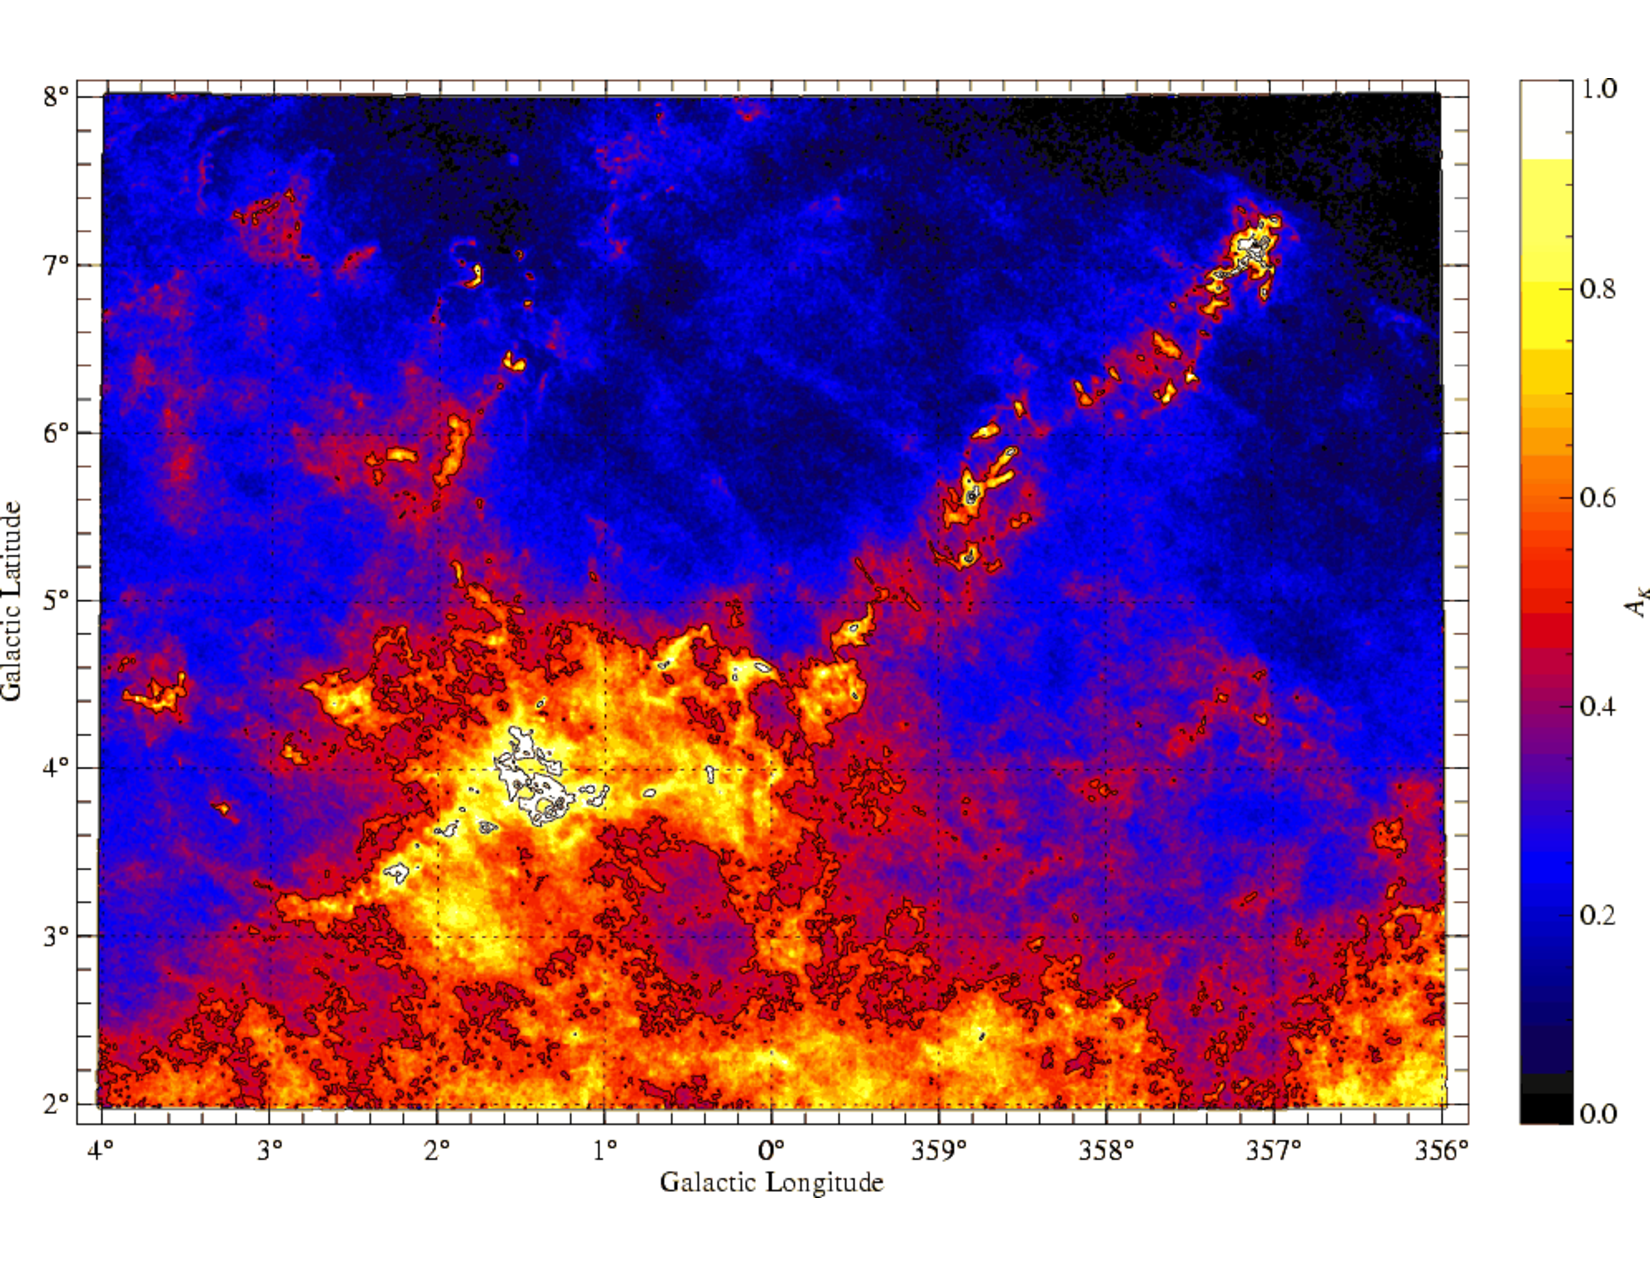
\includegraphics[width=\linewidth]{pipe_lombardi06}
\caption[Dust extinction map of the Pipe Nebula]{
\label{fig:pipe_lombardi06}
Extinction map of the Pipe Nebula. The color scale shows the extinction in K band. Credit: \citeauthor{lombardi06a}, A\&A, 454, 781, 2006, reproduced with permission \copyright\,ESO.
}
\end{figure}

The advantages of this compared to dust thermal emission are threefold. First, since stars are bright compared to interstellar dust grains, and the observations are done in the near IR rather than the sub-mm, the available resolution is much, much higher. Second, since opacity doesn't depend on temperature, the uncertainty in converting what we see into a column density is reduced. Third, we know the dust opacity curve in the near infrared considerably better than we know it in the far-IR or sub-mm, further reducing the uncertainty. However, there are also drawbacks to this method. Due to the comparatively higher opacity in the infrared, it is only possible to use this technique for fairly diffuse regions; in denser regions the background stars are completely extincted. Moreover, one needs a good, clean field of background stars to get something like a map, and only a few clouds have such favorable geometry.


\subsection{Molecular Lines}
\label{ssec:molecular_lines}

Much of what we know about star forming gas comes from observations of line emission. These are usually the most complex measurements in terms of the modeling and theory required to understand them. However, they are also by far the richest in terms of the information they provide. They are also among the most sensitive, since the lines can be very bright compared to continuum emission. Indeed, the great majority of what we know about the ISM beyond the local group comes from studying emission in the rotational lines of the CO molecule, because these (plus the C~\textsc{ii} line found in atomic regions) are by far the easiest types of emission to detect from the cold ISM.

The simplest line-emitting system is an atom or molecule with exactly two energy states, but this example contains most of the concepts we will need. The generalization of these results to a multi-level system is given in Appendix \ref{app:multilevel_atoms}.

\paragraph{Einstein Coefficients and Collision Rates}

Consider an atom or molecule of species $X$ with two non-degenerate states that are separated by an energy $E$. Suppose we have a gas of such particles with number density $n_X$ at temperature $T$. The number density of atoms in the ground state is $n_0$ and the number density in the excited state is $n_1$. At first suppose that this system does not radiate. In this case collisions between the atoms will eventually bring the two energy levels into thermal equilibrium, and it is straightforward to compute $n_0$ and $n_1$. They just follow a Maxwellian distribution, so $n_1/n_0 = e^{-E/k_B T}$, and thus we have $n_0 = n_X /Z$ and $n_1 = n_X e^{-E/k_B T}/Z$, where $Z=1+e^{-E/k_B T}$ is the partition function.

Now let us consider radiative transitions between these states. There are three processes: spontaneous emission, stimulated emission, and absorption, which are described by the three Einstein coefficients. In studying star formation, we can often ignore stimulated emission and absorption, because the ambient radiation field is so weak that these processes occur at negligible rates. The exception to this is when lines become optically thick, so there are a lot of line photons bouncing around trapped inside a structure, or when the frequency of the transition in question is at very low energy, and interactions with CMB photons become significant. However, for simplicity we will begin by just focusing on spontaneous emission and ignoring absorption and stimulated emission. The full statistical mechanics problem including these processes is discussed in Appendix \ref{app:multilevel_atoms}.

An atom in the excited state can spontaneously emit a photon and decay to the ground state. The rate at which this happens is described by the Einstein coefficient $A_{10}$, which has units of s$^{-1}$. Its meaning is simply that a population of $n_1$ atoms in the excited state will decay to the ground state by spontaneous emission at a rate 
\begin{equation}
\left(\frac{dn_1}{dt}\right)_{\rm spon.~emis.} = -A_{10} n_1.
\end{equation}
In cgs units this quantity is measured in atoms per cm$^3$ per s, and this expression is equivalent to saying that the $e$-folding time for decay is $1/A_{10}$ seconds. For most of the molecules we will be considering in this book, decay times are typically at most a few centuries, which is short compared to pretty much any time scale associated with star formation. Thus if spontaneous emission were the only process at work, all molecules would quickly decay to the ground state and we wouldn't see any emission.

However, in the dense interstellar environments where stars form, collisions occur frequently enough to create a population of excited molecules. Of course collisions involving excited molecules can also cause de-excitation, with the excess energy going into recoil rather than into a photon. Since hydrogen molecules are almost always the most abundant species in the dense regions we're going to think about, with helium second, we can generally only consider collisions between our two-level atom and those partners. For the purposes of this exercise, we'll take an even simpler approach and ignore everything but H$_2$. Putting He back into the picture is easy, as it just requires adding extra collision terms that are completely analogous to the ones we will write down.

The rate at which collisions cause transitions between states is a horrible quantum mechanical problem. We cannot even confidently calculate the energy levels of single isolated molecules except in the simplest cases, let alone the interactions between two colliding ones at arbitrary velocities and relative orientations. Exact calculations of collision rates are generally impossible. Instead, we either make due with approximations (at worst), or we try to make laboratory measurements. Things are bad enough that, for example, we often assume that the rates for collisions with H$_2$ molecules and He atoms are related by a constant factor.

Fortunately, as astronomers we generally leave these problems to chemists, and instead do what we always do: hide our ignorance behind a parameter. We let the rate at which collisions between species $X$ and H$_2$ molecules induce transitions from the ground state to the excited state be
\begin{equation}
\left(\frac{dn_1}{dt}\right)_{\rm coll.~exc.} = k_{01} n_0 n,
\end{equation}
where $n$ is the number density of H$_2$ molecules and $k_{01}$ has units of cm$^3$ s$^{-1}$. In general $k_{01}$ will be a function of the gas kinetic temperature $T$, but not of $n$ (unless $n$ is so high that three-body processes start to become important, which is almost never the case in the ISM). 

The corresponding rate coefficient for collisional de-excitation is $k_{10}$, and the collisional de-excitation rate is
\begin{equation}
\left(\frac{dn_1}{dt}\right)_{\rm coll.~de-exc.} = -k_{10} n_1 n.
\end{equation}
A little thought should suffice to convince the reader that $k_{01}$ and $k_{10}$ must have a specific relationship. Consider an extremely dense region where $n$ is so large that collisional excitation and de-excitation both occur much, much more often than spontaneous emission, and we can therefore neglect the spontaneous emission term in comparison to the collisional ones. If the gas is in equilibrium then we have
\begin{eqnarray}
\frac{dn_1}{dt} = \left(\frac{dn_1}{dt}\right)_{\rm coll.~exc.} + \left(\frac{dn_1}{dt}\right)_{\rm coll.~de-exc.} & = & 0 \\
n (k_{01} n_0 - k_{10} n_1) & = & 0.
\end{eqnarray}
However, we also know that the equilibrium distribution is a Maxwellian, so $n_1/n_0 = e^{-E/k_B T}$. Thus we have
\begin{eqnarray}
n n_0 (k_{01} - k_{10} e^{-E/k_B T}) & = & 0 \\
k_{01} & = & k_{10} e^{-E/k_B T}.
\label{eq:detailed_balance}
\end{eqnarray}
This argument applies equally well between a pair of levels even for a complicated molecule with many levels instead of just 2. Thus, we only need to know the rate of collisional excitation or de-excitation between any two levels to know the reverse rate.

\paragraph{Critical Density and Density Inference}

We are now in a position to write down the full equations of statistical equilibrium for the two-level system. In so doing, we will see that we can immediately use line emission to learn a great deal about the density of gas. In equilibrium we have
\begin{eqnarray}
\frac{dn_1}{dt} & = & 0 \\
n_1 A_{10} + n n_1 k_{10} -n n_0 k_{01} & = & 0 \\
\frac{n_1}{n_0} \left(A_{10} + k_{10}n\right) - k_{01} n & = & 0\\
\frac{n_1}{n_0} & = & \frac{k_{01} n}{A_{10}+k_{10} n}\\
& = & e^{-E/k_B T} \frac{1}{1+A_{10}/(k_{10} n)}
\end{eqnarray}
This physical meaning of this expression is clear. If radiation is negligible compared to collisions, i.e., $A_{10} \ll k_{10} n$, then the ratio of level populations approaches the Maxwellian ratio $e^{-E/k_B T}$. As radiation becomes more important, i.e., $A_{10}/(k_{10} n)$ get larger, the fraction in the upper level drops -- the level population is sub-thermal. This is because radiative decays remove molecules from the upper state faster than collisions re-populate it.

Since the collision rate depends on density and the radiative decay rate does not, the balance between these two processes depends on density. This make it convenient to introduce a critical density $n_{\rm crit}$, defined by
\begin{equation}
\label{eq:ncrit}
n_{\rm crit} = \frac{A_{10}}{k_{10}},
\end{equation}
so that
\begin{equation}
\frac{n_1}{n_0} = e^{-E/k_B T} \frac{1}{1+n_{\rm crit}/n}.
\end{equation}
At densities much larger than $n_{\rm crit}$, we expect the level population to be close to the Maxwellian value, and at densities much smaller than $n_{\rm crit}$ we expect the upper state to be under-populated relative to Maxwellian; $n_{\rm crit}$ itself is simply the density at which radiative and collisional de-excitations out of the upper state occur at the same rate.

This process of thermalization has important consequences for the line emission we see from molecules. The energy emission rate per molecule from the line is 
\begin{eqnarray}
\frac{\mathcal{L}}{n_X} & = & \frac{E A_{10} n_1}{n_X} \\
& = & E A_{10} \frac{n_1}{n_0+n_1} \\
& = & E A_{10} \frac{n_1/n_0}{1+n_1/n_0} \\
& = & E A_{10} \frac{e^{-E/k_B T}}{1+e^{-E/k_B T}+n_{\rm crit}/n} \\
& = & E A_{10} \frac{e^{-E/k_B T}}{Z+n_{\rm crit}/n}
\end{eqnarray}
where again $Z$ is the partition function.

It is instructive to think about how this behaves in the limiting cases $n \ll n_{\rm crit}$ and $n\gg n_{\rm crit}$. In the limit $n\gg n_{\rm crit}$, the partition function $Z$ dominates the denominator, and we get $\mathcal{L}/n_X = E A_{10} e^{-E/k_B T}/Z$. This is just the energy per spontaneous emission, $E$, times the spontaneous emission rate, $A_{10}$, times the fraction of the population in the upper state when the gas is in statistical equilibrium, $e^{-E/k_B T}/Z$. This is density-independent, so this means that at high density the gas produces a fixed amount of emission per molecule of the emitting species. The total luminosity is just proportional to the number of emitting molecules.

For $n \ll n_{\rm crit}$, the second term dominates the denominator, and we get
\begin{equation}
\label{eq:cool_lowden}
\frac{\mathcal{L}}{n_X} \approx E A_{10} e^{-E/k_B T} \frac{n}{n_{\rm crit}}.
\end{equation}
Thus at low density each molecule contributes an amount of light that is proportional to the ratio of density to critical density. Note that this is the ratio of collision partners, i.e., of H$_2$, rather than the density of emitting molecules. The total luminosity varies as this ratio times the number of emitting molecules.

The practical effect of this is that different molecules tell us about different densities of gas in galaxies. Molecules with low critical densities reach the linear regime at low density, and since most of the mass tends to be at lower density, they probe this widespread, low-density component. Molecules with higher critical densities will have more of their emission contributed by higher density gas, and thus tell us about rarer, higher-density regions. This is all somewhat qualitative, since a transition between $\mathcal{L}/n_X \propto n$ and $\mathcal{L}/n_X \sim\mbox{constant}$ doesn't represent a particularly sharp change in behavior. Nonetheless, the luminosity ratios of lines with different critical densities are a very important diagnostic of the overall density distribution in the ISM.

As a caution, we should note that this is computed for optically thin emission. If the line is optically thick, we can no longer ignore stimulated emission and absorption processes, and not all emitted photons will escape from the cloud. In this case the effective critical density is reduced by a factor of the optical depth. CO, the most-commonly used tracer molecule, is usually optically thick.

\paragraph{Velocity and Temperature Inference}

We can also use molecular lines to infer the velocity and temperature structure of gas if the line in question is optically thin. For an optically thin line, the width of the line is determined primarily by the velocity distribution of the emitting molecules. The physics here is extremely simple. Suppose we have gas along our line of sight with a velocity distribution $\psi(v)$, i.e., the fraction of gas with velocities between $v$ and $v+dv$ is $\psi(v) dv$, and $\int_{-\infty}^{\infty} \psi(v) \, dv = 1$.

For an optically thin line, in the limit where natural and pressure-broadening of lines is negligible, which is almost always the case when observing the cold, dense, ISM, we can think of emission producing a delta function in frequency in the rest frame of the gas. There is a one-to-one mapping between velocity and frequency. Thus emission from gas moving at a velocity $v$ relative to us along our line of sight produces emission at a frequency $\nu \approx \nu_0 (1 - v/c)$, where $\nu_0$ is the central frequency of the line in the molecule's rest frame, and we assume $v/c \ll 1$. In this case the line profile is described trivially by $\phi(\nu)=\psi(c(1-\nu/\nu_0))$. 

We can measure $\phi(\nu)$ directly, and this immediately tells us the velocity distribution $\psi(v)$. In general the velocity distribution of the gas $\psi(v)$ is produced by a combination of thermal and non-thermal motions. Thermal motions arise from the Maxwellian velocity distribution of the gas, and produce a Maxwellian profile $\phi(\nu)\propto e^{-(\nu-\nu_{\rm cen})^2/2\sigma_\nu^2}$. Here $\nu_{\rm cen}$ is the central frequency of the line, which is $\nu_{\rm cen} = \nu_0 (1 - \bar{v}/c)$, where $\bar{v}$ is the mean velocity of the gas along our line of sight. The width is $\sigma_\nu = \nu_0 c^{-1}\sqrt{k_B T/\mu m_{\rm H}}$, where $T$ is the gas temperature and $\mu$ is the mean mass of the emitting molecule in units of hydrogen masses. This is just the 1D Maxwellian distribution.

Non-thermal motions involve bulk flows of the gas, and can produce a variety of velocity distributions depending how the cloud is moving. Unfortunately even complicated motions often produce distributions that look something like Maxwellian distributions, just because of the central limit theorem: if you throw together a lot of random junk, the result is usually a Gaussian / Maxwellian distribution. Figure \ref{fig:complete_ridge06} shows an example of velocity distributions measured in two nearby star-forming clouds.

\begin{marginfigure}
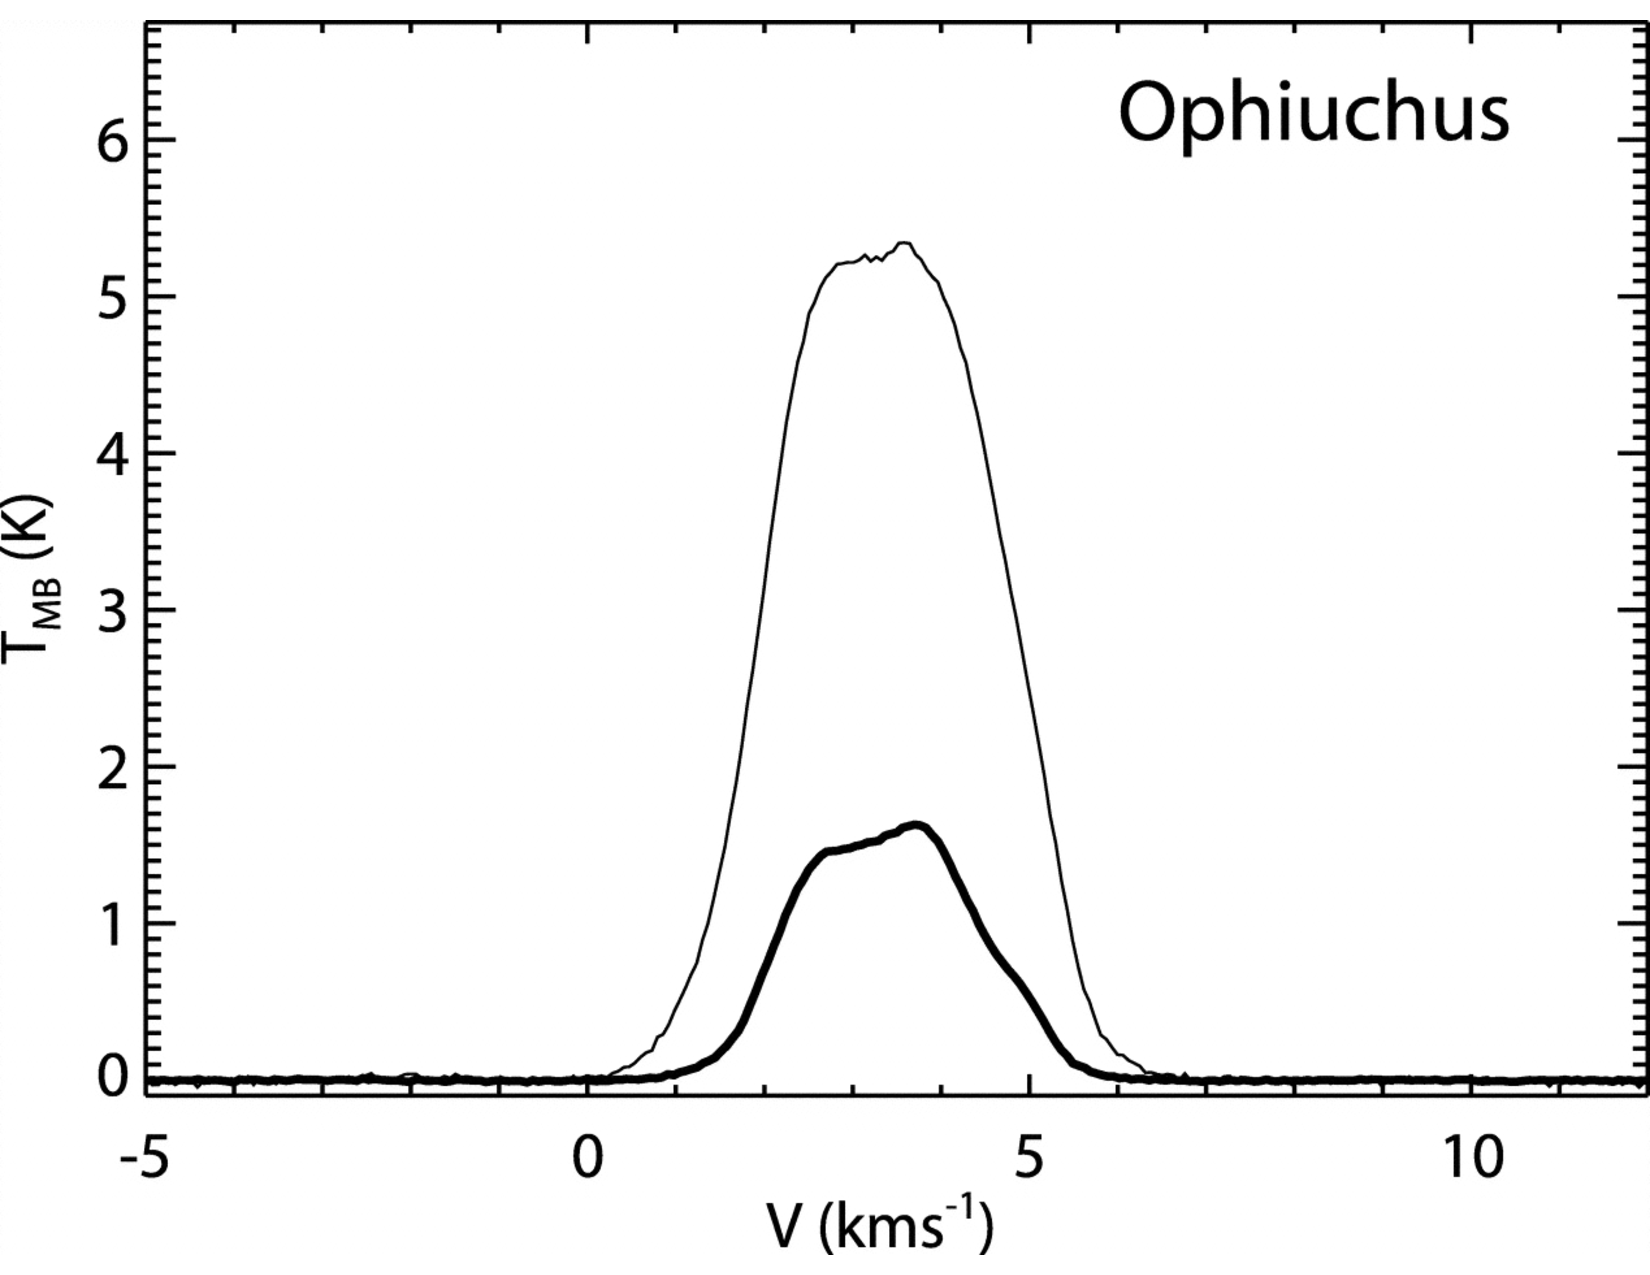
\includegraphics[width=\linewidth]{complete_ridge06a}
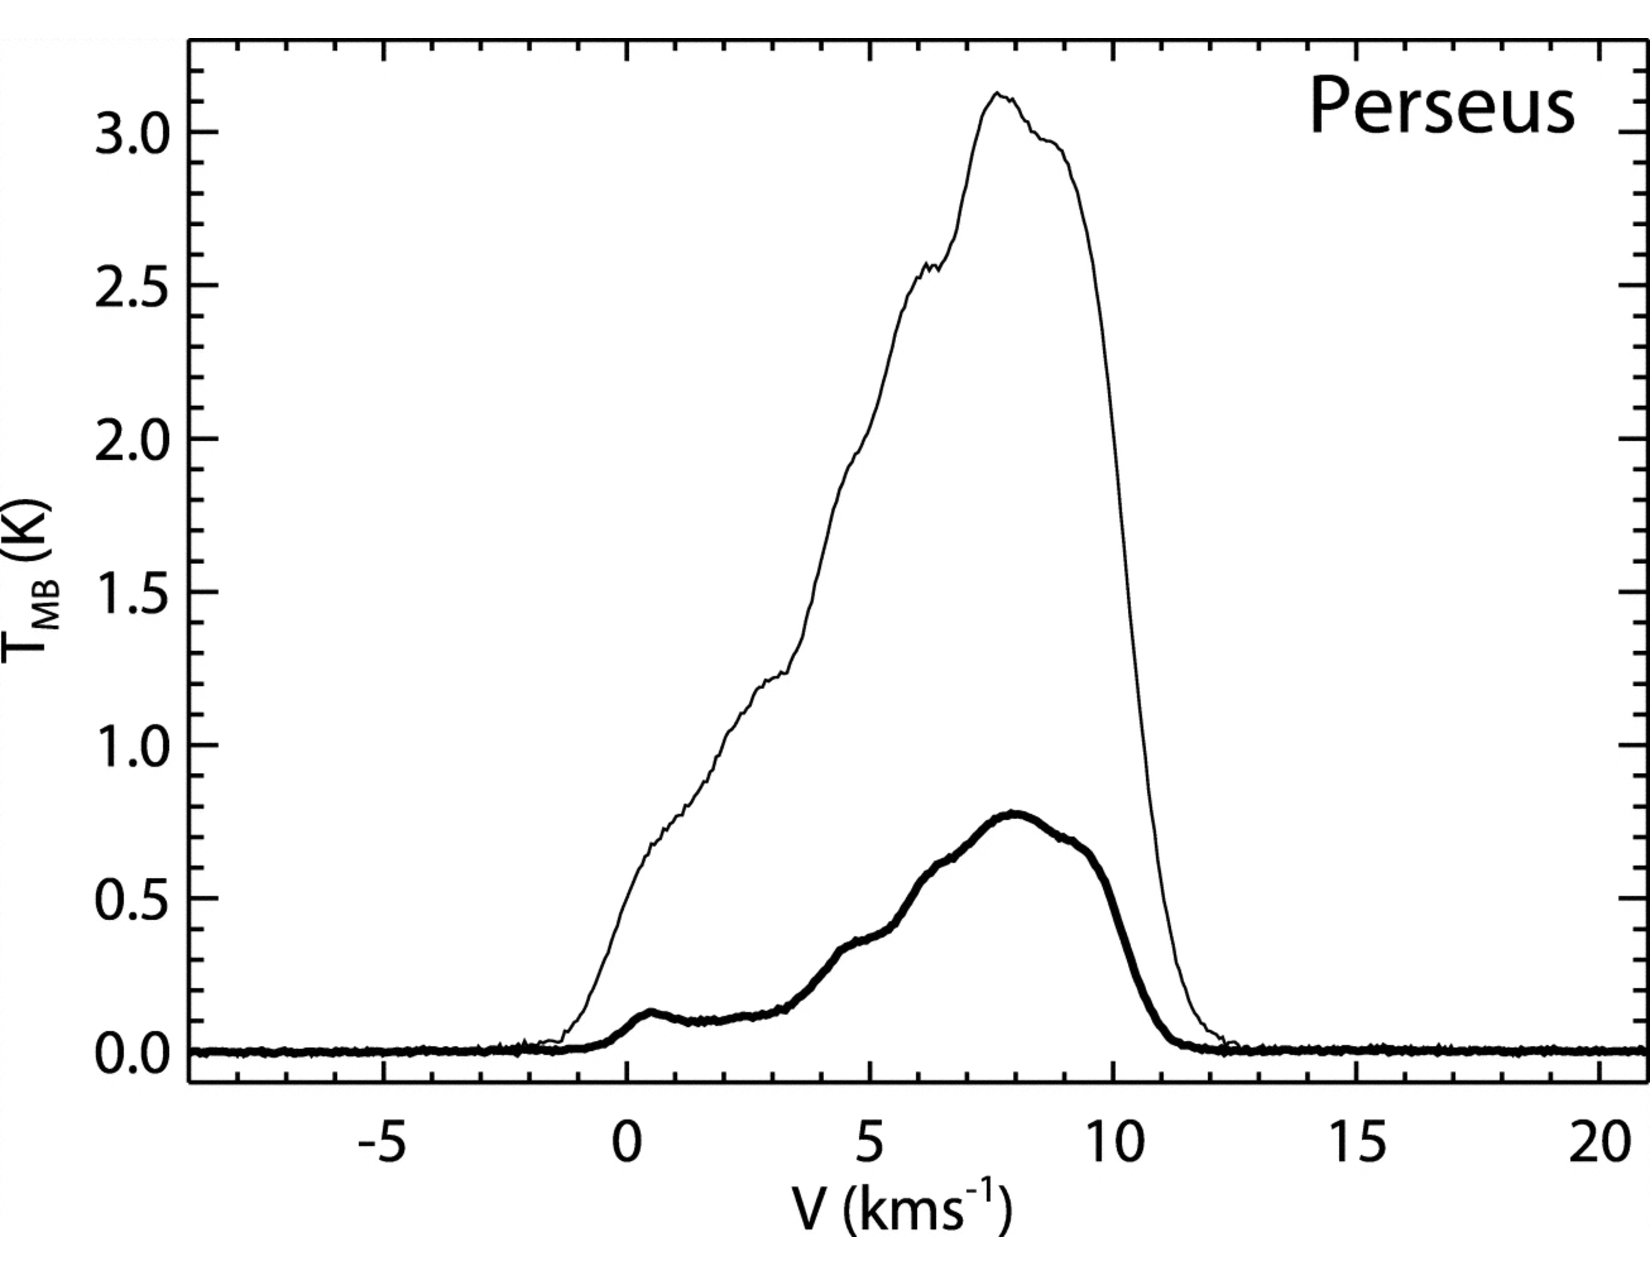
\includegraphics[width=\linewidth]{complete_ridge06b}
\caption[COMPLETE spectra of Ophiuchus and Perseus]{
\label{fig:complete_ridge06}
Position-integrated velocity distributions of $^{12}$CO (\textit{thin lines}) and $^{13}$CO (\textit{thick lines}) for the Ophiuchus and Perseus clouds, measured the COMPLETE survey. The $y$ axis shows the beam temperature. Credit: \citet{ridge06a}, \copyright\, AAS. Reproduced with permission.
}
\end{marginfigure}

Determining whether a given line profile reflects predominantly thermal or non-thermal motion requires that we have a way of estimating the temperature independently. This can often be done by observing multiple lines of the same species. Our expression
\begin{equation}
\frac{\mathcal{L}}{n_X} = E A_{10} \frac{e^{-E/k_B T}}{Z + n_{\rm crit}/n}
\end{equation}
shows that the luminosity of a particular optically thin line is a function of the temperature $T$, the density $n$, and the number density of emitting molecules $n_X$. If we observe three transitions of the same molecule, then we have three equations in three unknowns and we can solve for $n$, $n_X$, and $T$ independently. Certain molecules, because of their level structures, make this technique particularly clean. The most famous example of this is ammonia, NH$_3$.

\paragraph{Complications}

Before moving on it is worth mentioning some complications that make it harder to interpret molecular line data. The first is optical depth: for many of the strongest lines and most abundant species, the line becomes optically thick. As a result observations in the line show only the surface a given cloud; emission from the back side of the cloud is absorbed by the front side. One can still obtain useful information from optically thick lines, but it requires a bit more thought. We will return to the topic of what we can learn from optically thick lines in Chapter \ref{ch:gmcs}.

The second complication is chemistry and abundances. The formation and destruction of molecules in the ISM is a complicated problem, and in general the abundance of any given species depends on the density, temperature, and radiation environment of the the gas. At the edges of clouds, certain molecules may not be present because they are dissociated by the interstellar UV field. At high densities and low temperatures, many species freeze out onto the surfaces of dust grains. This is true for example of CO. One often sees that peaks in density found in dust emission maps correspond to local minima of CO emission. This is because in the densest parts of clouds CO goes out of the gas phase and forms CO ice on the surfaces of dust grains.  Thus one must always be careful to investigate whether changes in molecular line emission are due to changes in gas bulk properties (e.g., density, temperature) or due to changes in the abundance of the emitting species.


\section{Observational Phenomenology}

\subsection{Giant Molecular Clouds}

As discussed above, we usually cannot observe H$_2$ directly, so we are forced to do so by proxy. The most common proxy is the rotational lines of CO. These are useful because CO is the single most abundant molecule in the ISM after H$_2$, it tends to be found in the same places as H$_2$ (for reasons that will become clear in Chapter \ref{ch:microphysics}, and the CO molecule has a number of transitions that can be excited at the low temperatures found in molecular clouds -- for example the CO $J=1$ state is only 5.5 K above the ground state. Indeed, the CO molecule is the primary coolant of molecular gas, so its excitation in effect sets the molecular gas temperature. 

In Chapter \ref{ch:gmcs} we will discuss how one infers the mass of an observed gas cloud from CO emission, and for the moment we will take it for granted that one can do so. By mass the Milky Way's ISM inside the solar circle is roughly 70\% H~\textsc{i} and 30\% H$_2$. The molecular fraction rises sharply toward the galactic center, reaching near unity in the molecular ring at $\sim 3$ kpc, then falling to $\sim 10\%$ out where we are. In other nearby galaxies the proportions vary from nearly all H~\textsc{i} to nearly all H$_2$.

In galaxies that are predominantly H~\textsc{i}, like ours, the atomic gas tends to show a filamentary structure, with small clouds of molecular gas sitting on top of peaks in the H~\textsc{i} distribution. In galaxies with large-scale spiral structure, the molecular gas closely tracks the optical spiral arms. Figures \ref{fig:m33_imara} and \ref{fig:m51_schinnerer} show examples of the former and the latter, respectively. The physical reasons for the associations between molecular gas and H~\textsc{i}, and between molecular clouds and spiral arms, are an interesting point that we will discuss in Chapter \ref{ch:microphysics}. 

\begin{figure}
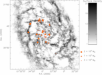
\includegraphics[width=\linewidth]{m33_imara}
\caption[Distribution of H~\textsc{i} and GMCs in M33]{
\label{fig:m33_imara}
Map of H~\textsc{i} in M33 (\textit{grayscale}), with giant molecular clouds detected in CO($1\rightarrow 0$) overlayed (\textit{circles}, sized by GMC mass). Credit: \citet{imara11b}, \copyright\, AAS. Reproduced with permission.
}
\end{figure}

\begin{figure}
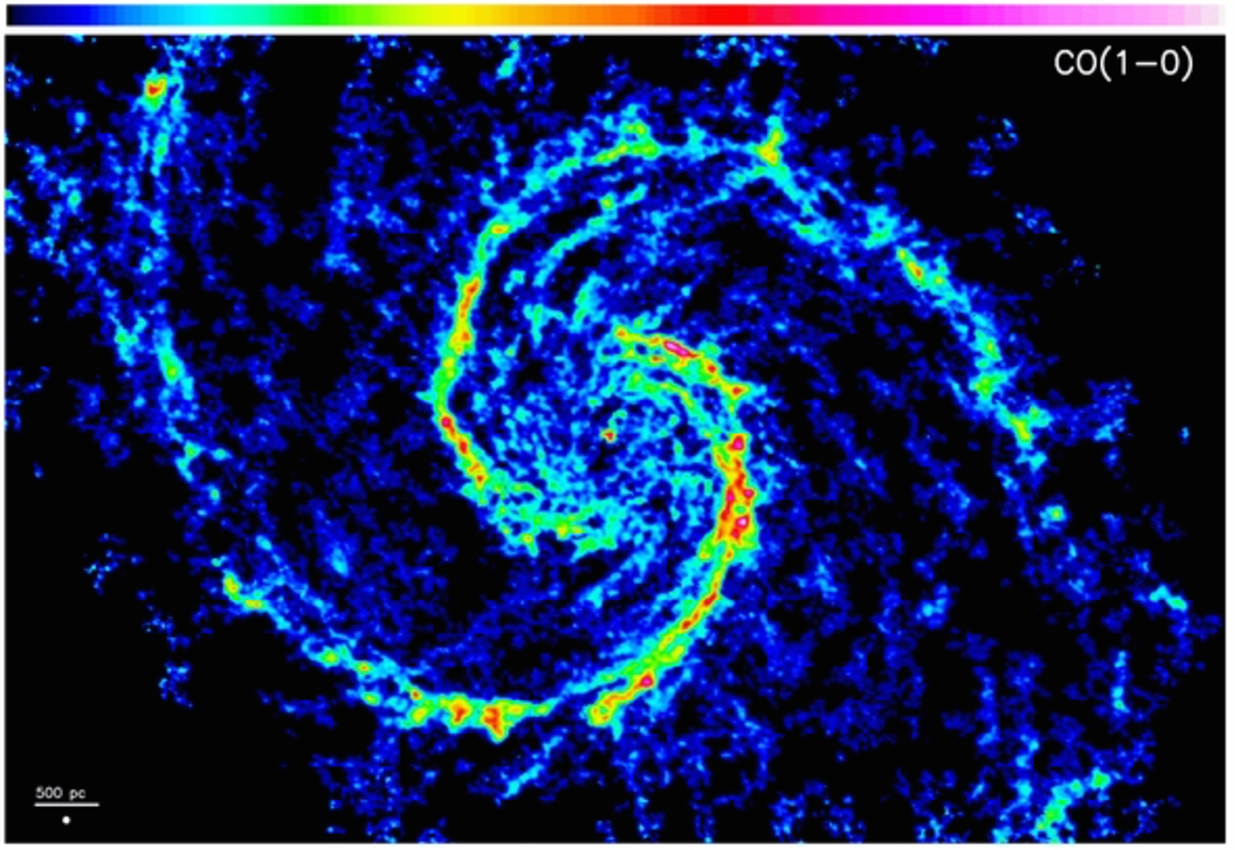
\includegraphics[width=\linewidth]{m51_schinnerer}
\caption[Distribution of CO($1\rightarrow 0$) emission in M51]{
\label{fig:m51_schinnerer}
Map of CO($1\rightarrow 0$) emission in M51, as measured by the PdBI Arcsecond Whirlpool Survey (PAWS) project. Credit: \citet{schinnerer13a}, \copyright\, AAS. Reproduced with permission.
}
\end{figure}

As the images show, molecular gas in galaxies that are predominantly atomic tends to be organized into discreet clouds, called giant molecular clouds (GMCs). These can have a range of masses; in the Milky Way the most massive are a few million $\msun$, but there is a spectrum that seems to continue down to at least $10^4$ $\msun$. This organization into GMCs is clearest where the gas is predominantly atomic. In regions where molecules make up most of the mass, the clouds begin to run together and it is no longer possible to identify discrete clouds in a meaningful way.

\subsection{Internal structure of GMCs}

Giant molecular clouds are not spheres. They have complex internal structures, as illustrated in Figure \ref{fig:perseus_sun06}. They tend to be highly filamentary and clumpy, with most of the mass in low density structures and only a little bit in very dense parts. However, if one computes a mean density by dividing the total mass by the rough volume occupied by the $^{12}$CO gas, the result is $\sim 100$ cm$^{-3}$. Typical size scales for GMCs are tens of pc -- the Perseus cloud shown in Figure \ref{fig:perseus_sun06} is a small one by Galactic standards, but the most massive ones are found predominantly in the molecular ring, so our high resolution images are all of nearby small ones.

\begin{figure}
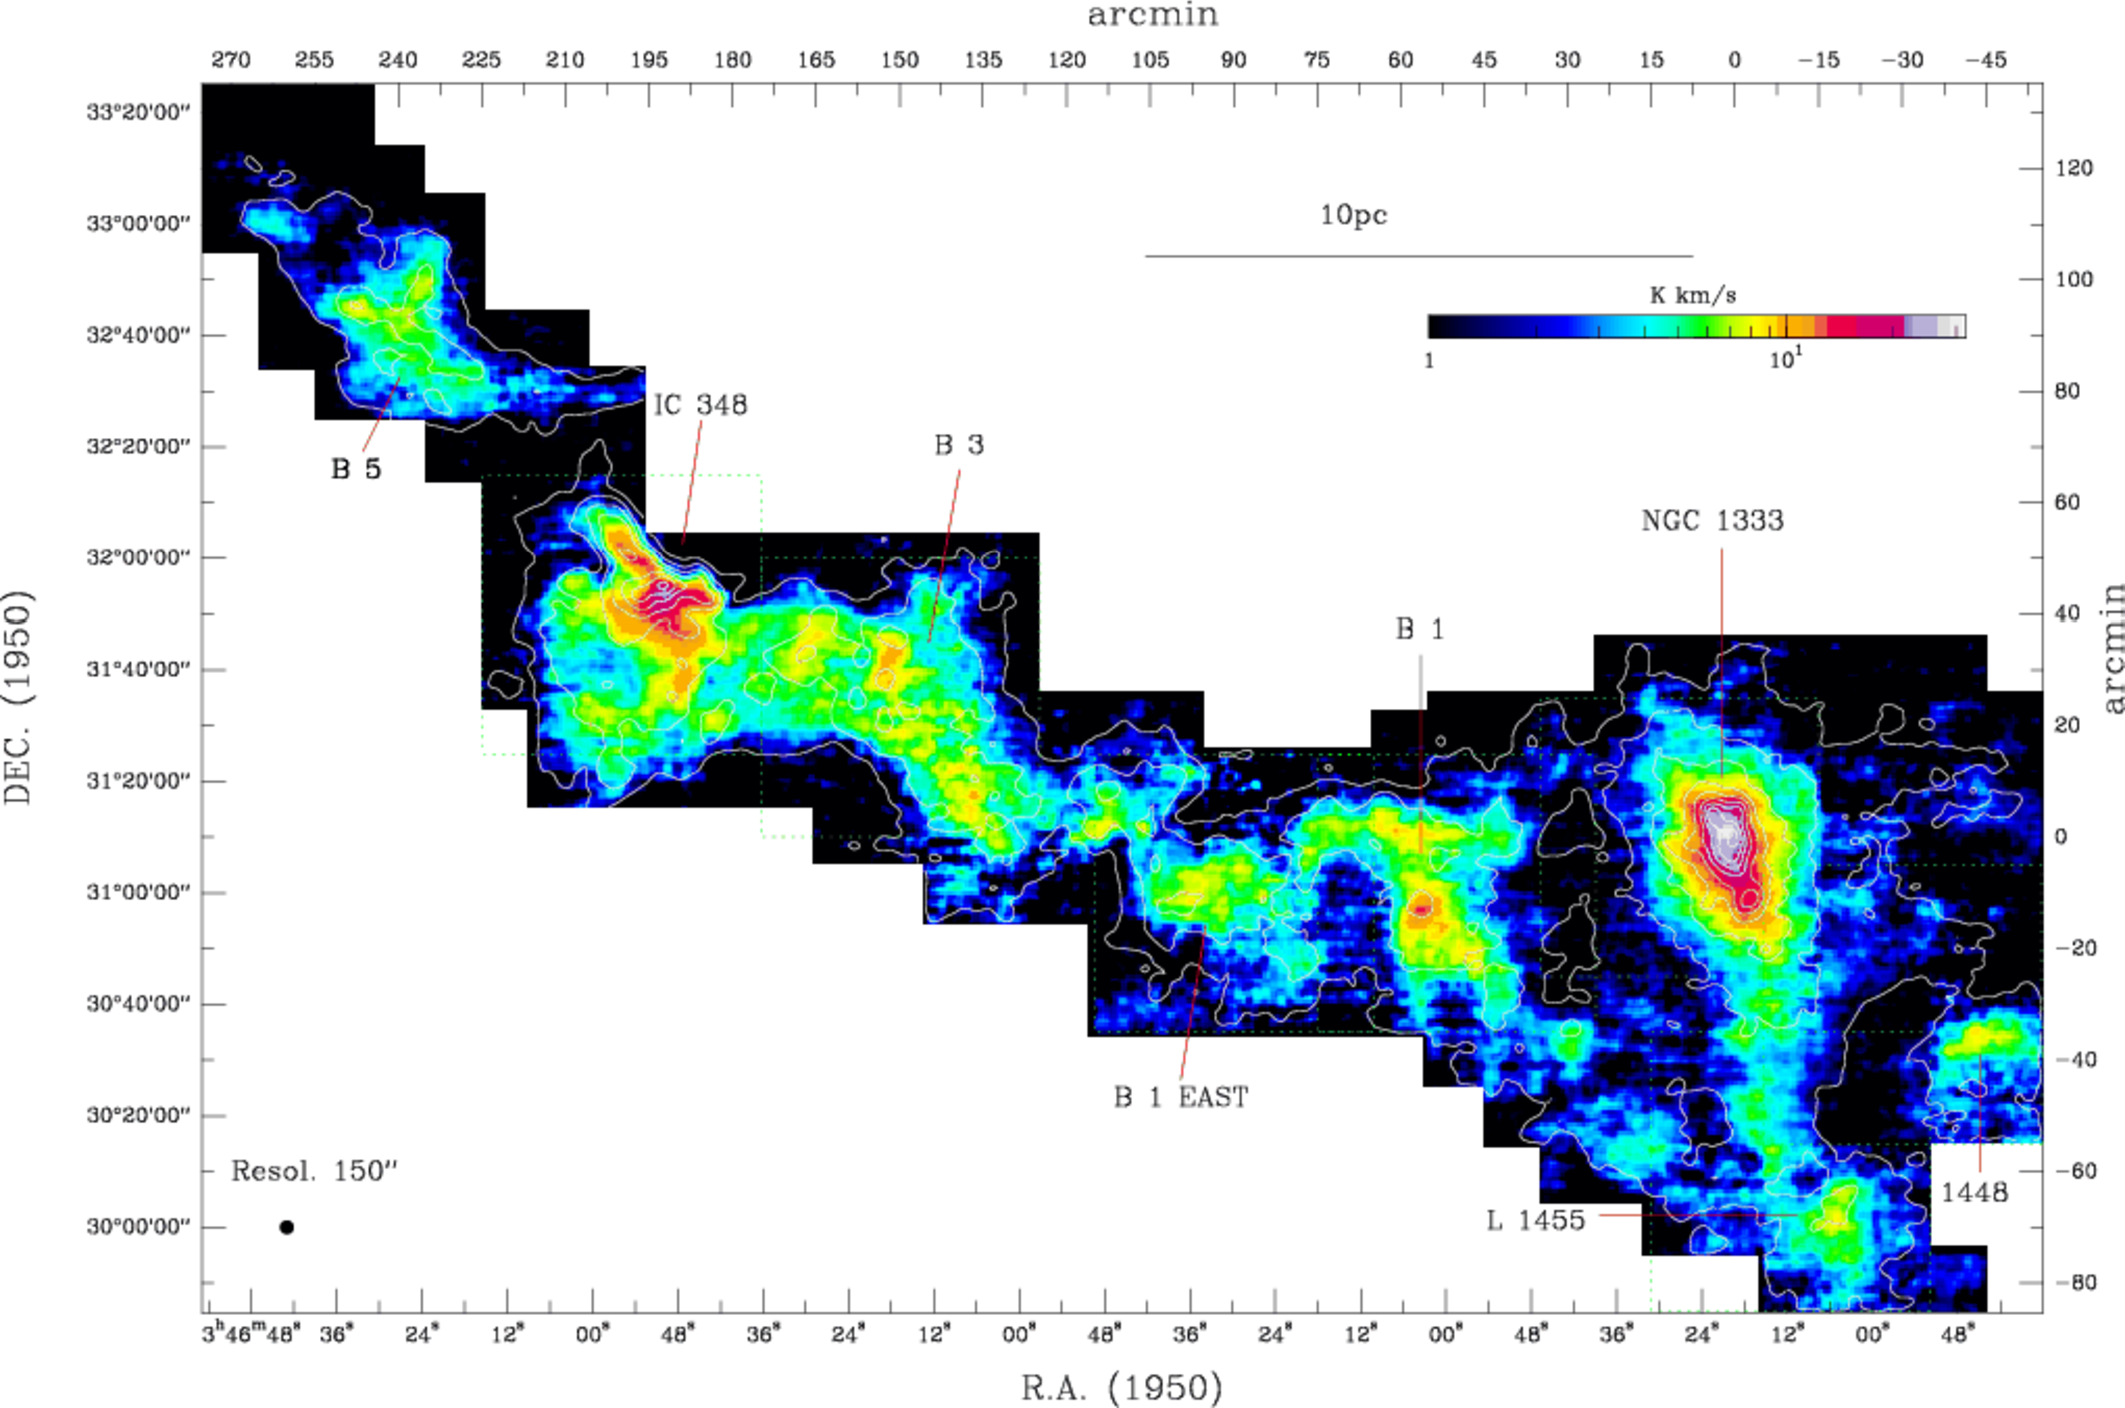
\includegraphics[width=\linewidth]{perseus_integrated_sun06}
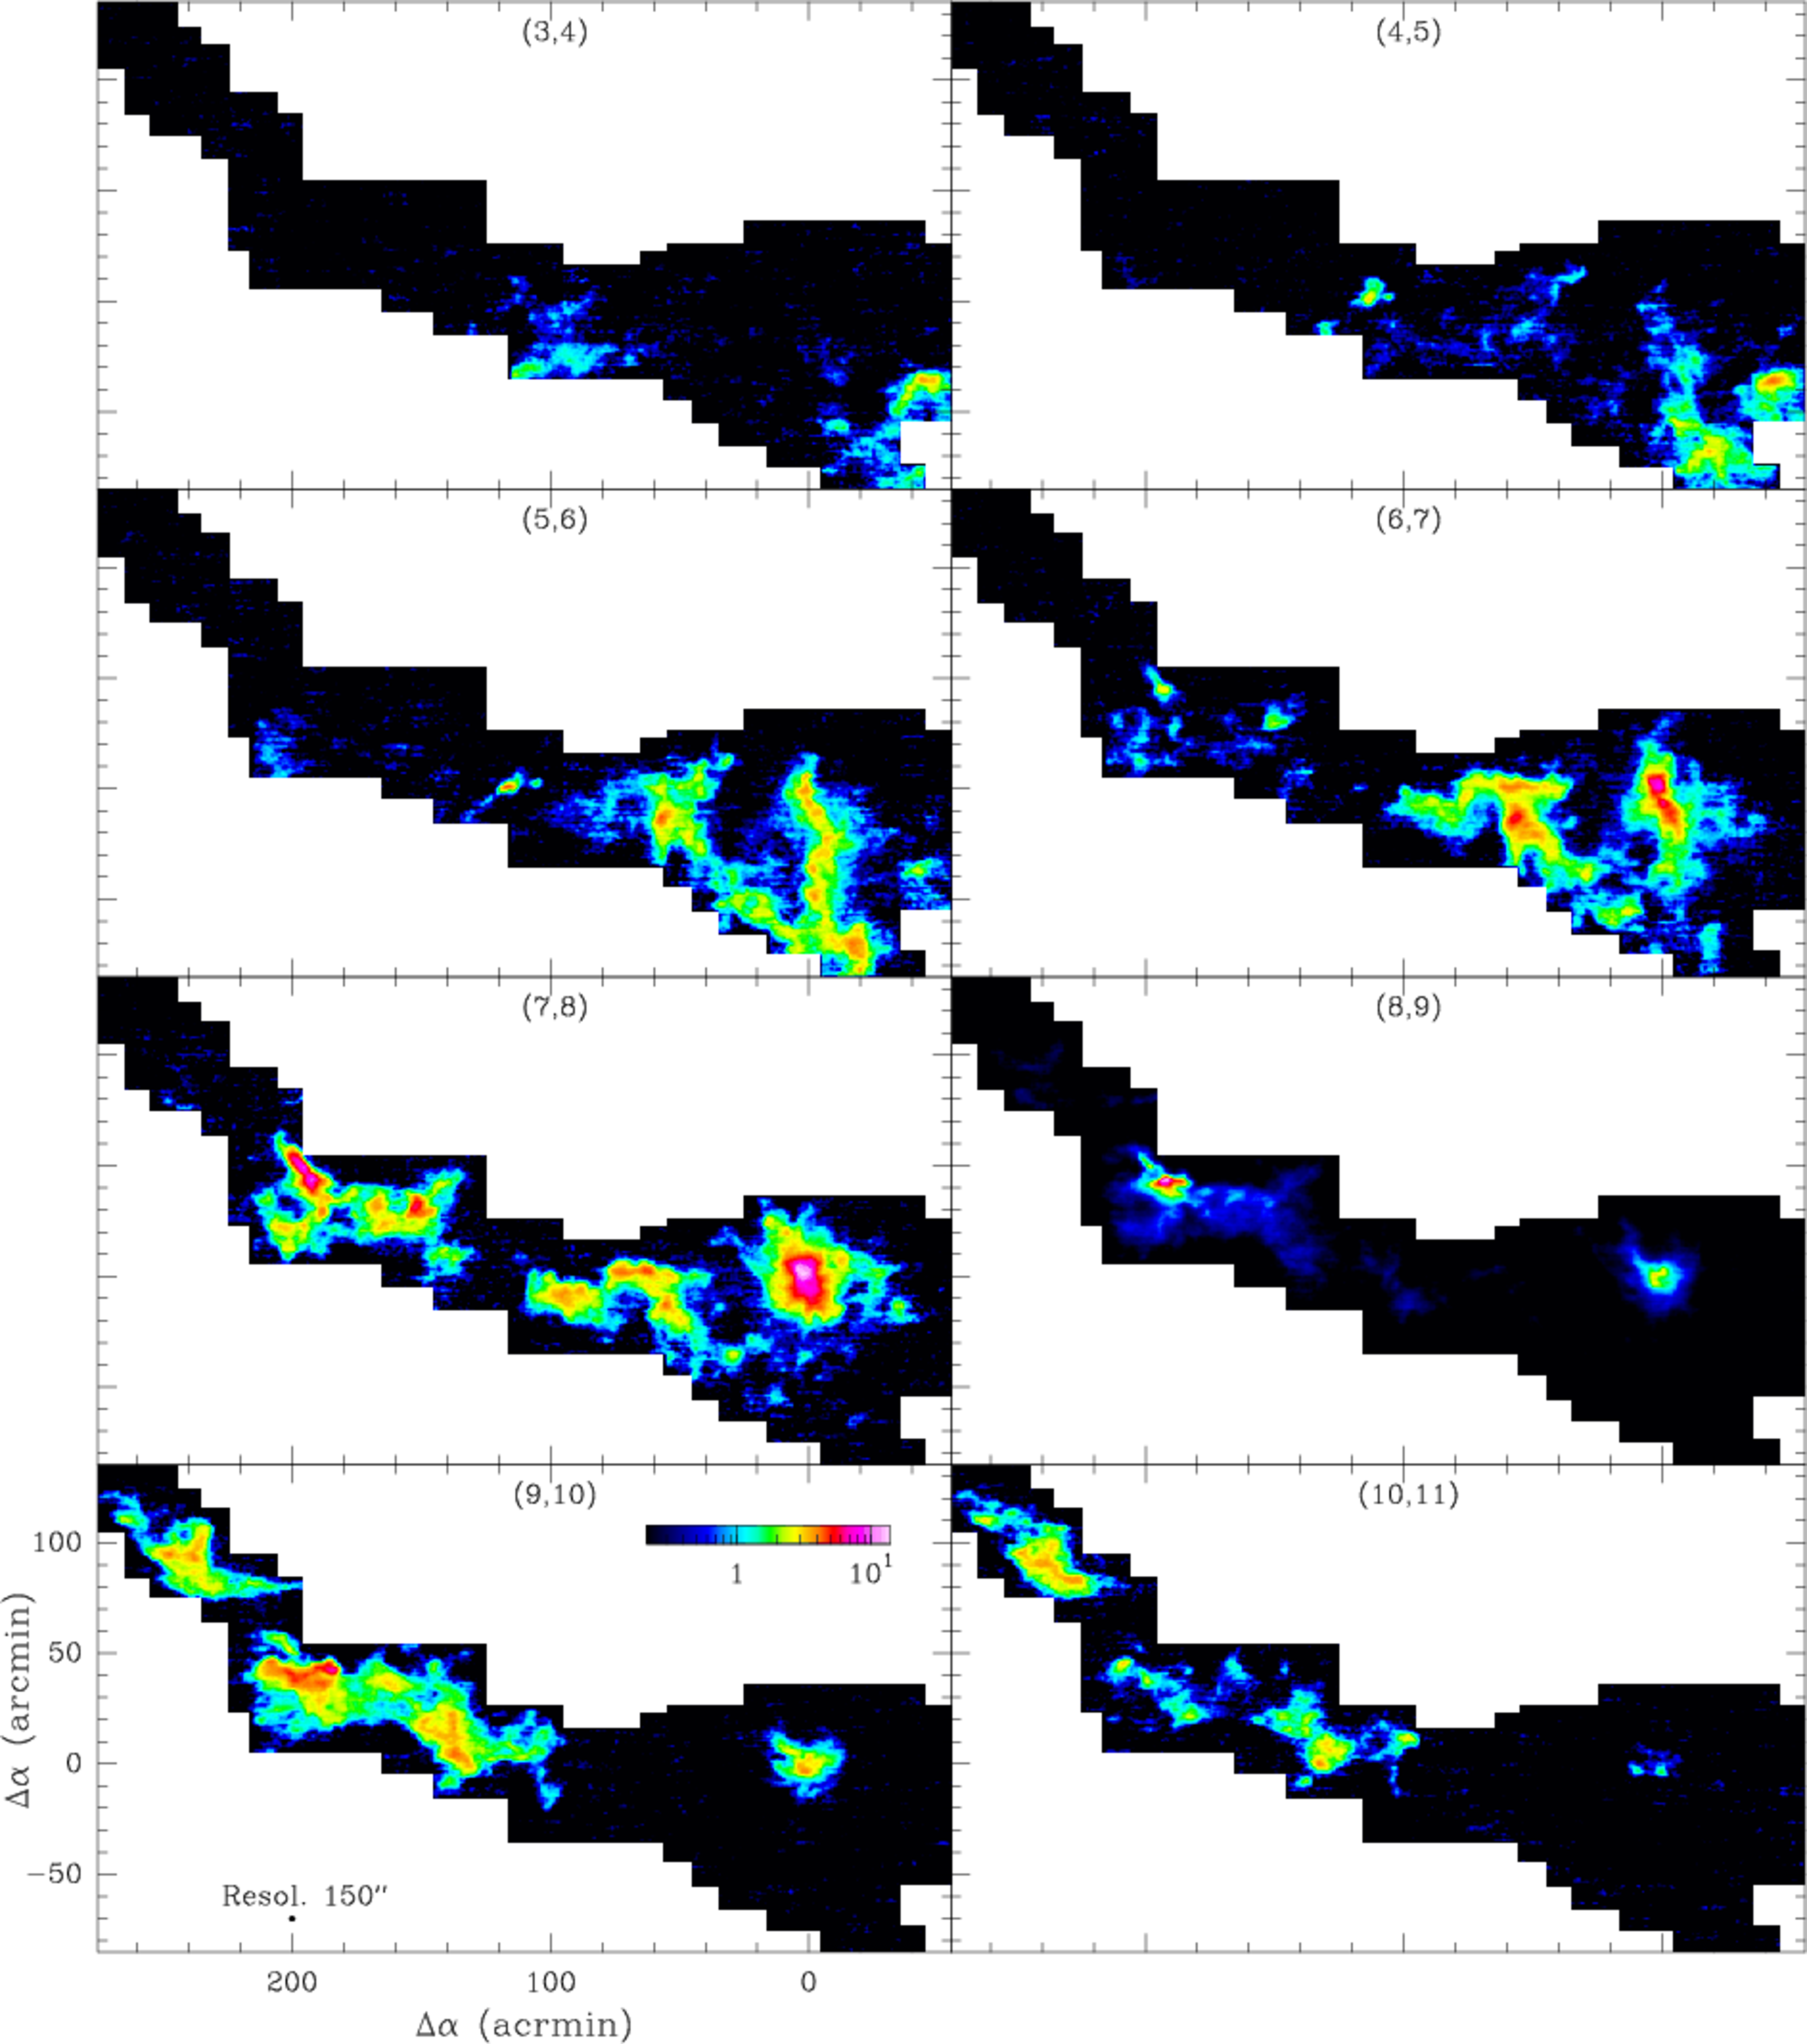
\includegraphics[width=\linewidth]{perseus_channel_sun06}
\caption[$^{13}$CO($2\rightarrow 1$) maps of Perseus]{
\label{fig:perseus_sun06}
Map of the Perseus cloud in $^{13}$CO($2\rightarrow 1$). The top panel shows the emission integrated over all velocities, while the bottom panel shows maps integrated over different velocity channels. In each sub-panel in the bottom, the numbers at the top indicate the velocity range (in km s$^{-1}$) of the emission shown. Credit: \citeauthor{sun06a}, A\&A, 451, 539, 2006, reproduced with
permission \copyright ESO.
}
\end{figure}

This complex structure on the sky is matched by a complex velocity structure. GMCs typically have velocity spreads that are much larger than the thermal sound speed of $\sim 0.2$ km s$^{-1}$ appropriate to 10 K gas. One can use different tracers to explore the distributions of gas at different densities in position-position-velocity space -- at every position one obtains a spectrum that can be translated into a velocity distribution along that line of sight. The data can be sliced into different velocities.

One can also get a sense of density and velocity structure by combining different molecular tracers. For example, the data set from COMPLETE (see Figure \ref{fig:complete_ridge06}) consists of three-dimensional cubes of $^{12}$CO and $^{13}$CO emission in position-position-velocity space, and from this one can draw isosurfaces. Generally the $^{12}$CO isosurfaces contain the $^{13}$CO ones, as expected since the $^{12}$CO traces less dense gas and the $^{13}$CO traces more dense gas. The density increases as one moves toward the cloud "center" in both position and velocity, but the morphology is not simple.   

\subsection{Cores}

As we zoom into yet smaller scales, the density rises to $10^5 - 10^7$ cm$^{-3}$ or more, while the mass decreases to a few $\msun$. These regions, called cores, tend to be strung out along filaments of lower density gas. Morphologically, cores tend to be closer to round than the lower-density material around them. These objects are thought to be the progenitors of single stars or star systems. Cores are distinguished not just by simple, roundish density structures, but by similarly simple velocity structures. Unlike in GMCs, where the velocity dispersion is highly supersonic, in cores it tends to be subsonic. This is indicated by a thermal broadening that is comparable to what one would expect from purely thermal motion.



\chapter{Observing Young Stars}
\label{ch:obsstars}

\marginnote{
\textbf{Suggested background reading:}
\begin{itemize}
\item \href{http://adsabs.harvard.edu/abs/2012ARA\%26A..50..531K}{Kennicutt, R.~C., \& Evans, N.~J. 2012, ARA\&A, 50, 531}, section 3 \nocite{kennicutt12a}
\item \href{http://adsabs.harvard.edu/abs/2014arXiv1402.0867K}{Krumholz, M.~R. 2014, Phys.~Rep., 539, 49}, section 2 \nocite{krumholz14c}
\end{itemize}
}

Having discussed how we observe interstellar gas that is forming stars, we now turn to the phenomenology of the young stars themselves. This chapter works form small to large scales, first discussing individual young stars, then resolved young stellar populations, and then ending with unresolved stellar populations in the Milky Way and nearby galaxies.

\section{Individual Stars}

Since we think star formation begins with a core that is purely gas, the first observable stage of star formation should be a cloud that is cold and lacks a central point source. Once a protostar forms, it will begin gradually heating up the cloud, while the gas in the cloud collapses onto the protostar, reducing the opacity. Eventually enough material accretes from the envelope to render it transparent in the near infrared and finally the optical, and we begin to be able to see the star directly for the first time. The star is left with an accretion disk, which gradually accretes and is then dispersed. Eventually the star contracts onto the main sequence.

This theoretical cartoon has been formalized into a system of classification of young stars based on observational diagnostics. At one end of this sequence lies purely gaseous sources where there is no evidence at all for the presence of a star, and at the other end lies ordinary main sequence stars. In between, objects are classified based on their emission in the infrared and sub-mm parts of the spectrum. These classifications probably give more of an impression of discrete evolutionary stages than is really warranted, but they nonetheless serve as a useful rough guide to the evolutionary state of a forming star.

Consider a core of mass $\sim 1$ $\msun$, seen in dust or molecular line emission. When a star first forms at its center, it will be very low mass and very low luminosity, and will heat up only the dust nearest to it, and only by a very small amount. Thus the total light output will still be dominated by the thermal emission of the dust at its equilibrium temperature. The spectral energy distribution of the source will therefore look just like that which prevailed before the star formed.

\begin{marginfigure}
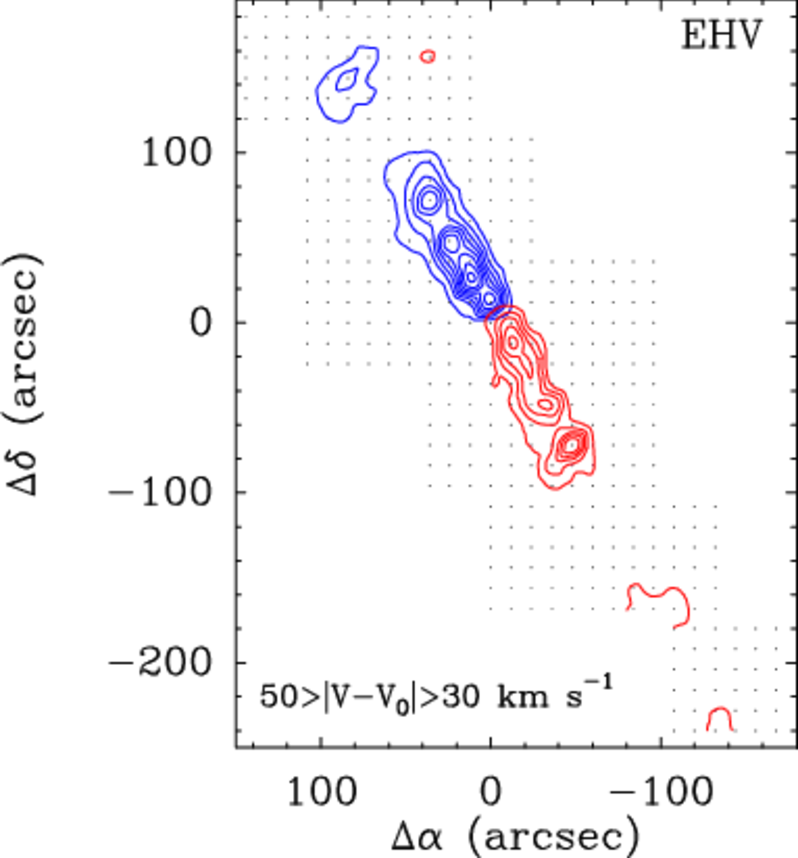
\includegraphics[width=\linewidth]{outflow_tafalla04}
\caption[Outflow in CO($2\rightarrow 1$)]{
\label{fig:outflow_tafalla04}
An integrated intensity map in CO($2\rightarrow 1$), showing material at velocities between $\pm 30-50$ km s$^{-1}$ (\textit{blue and red contours, respectively}) relative to the mean. Contours are spaced at intensities of 1 K km s$^{-1}$. The outflow shown is in the Taurus star-forming region. Credit: \citeauthor{tafalla04c}, A\&A,423, L21, 2004, reproduced with permission \copyright\, ESO.
}
\end{marginfigure}

However, there might be other indicators that a star has formed. For example, the density distribution might show a very sharp, unresolved peak. Another sign that a star has formed might be the presence of an outflow, which, as we discuss in Chapter \ref{ch:disks_obs}, all protostars seem to generate. Outflows coming from the center of a core can be detected in a few ways. Most directly, one can see bipolar, high velocity structures in molecular emission (Figure \ref{fig:outflow_tafalla04}). One can also detect indirect evidence of an outflow, from the presence of highly excited molecular line emission that is produced by shocks at hundreds of km s$^{-1}$. One example of such a line is SiO($2\rightarrow 1)$ line, which is generally seen in gas moving at several tens of km s$^{-1}$ with temperatures of several hundred K -- this is taken to be indication that emission in this line is produced in warm shocks. Since we know of no processes other than formation of a compact object with a $\gtrsim 100$ km s$^{-1}$ escape velocity that can accelerate gas in molecular clouds to such speeds, the presence of such an outflow is taken to indicate that a compact object has formed.

\begin{marginfigure}
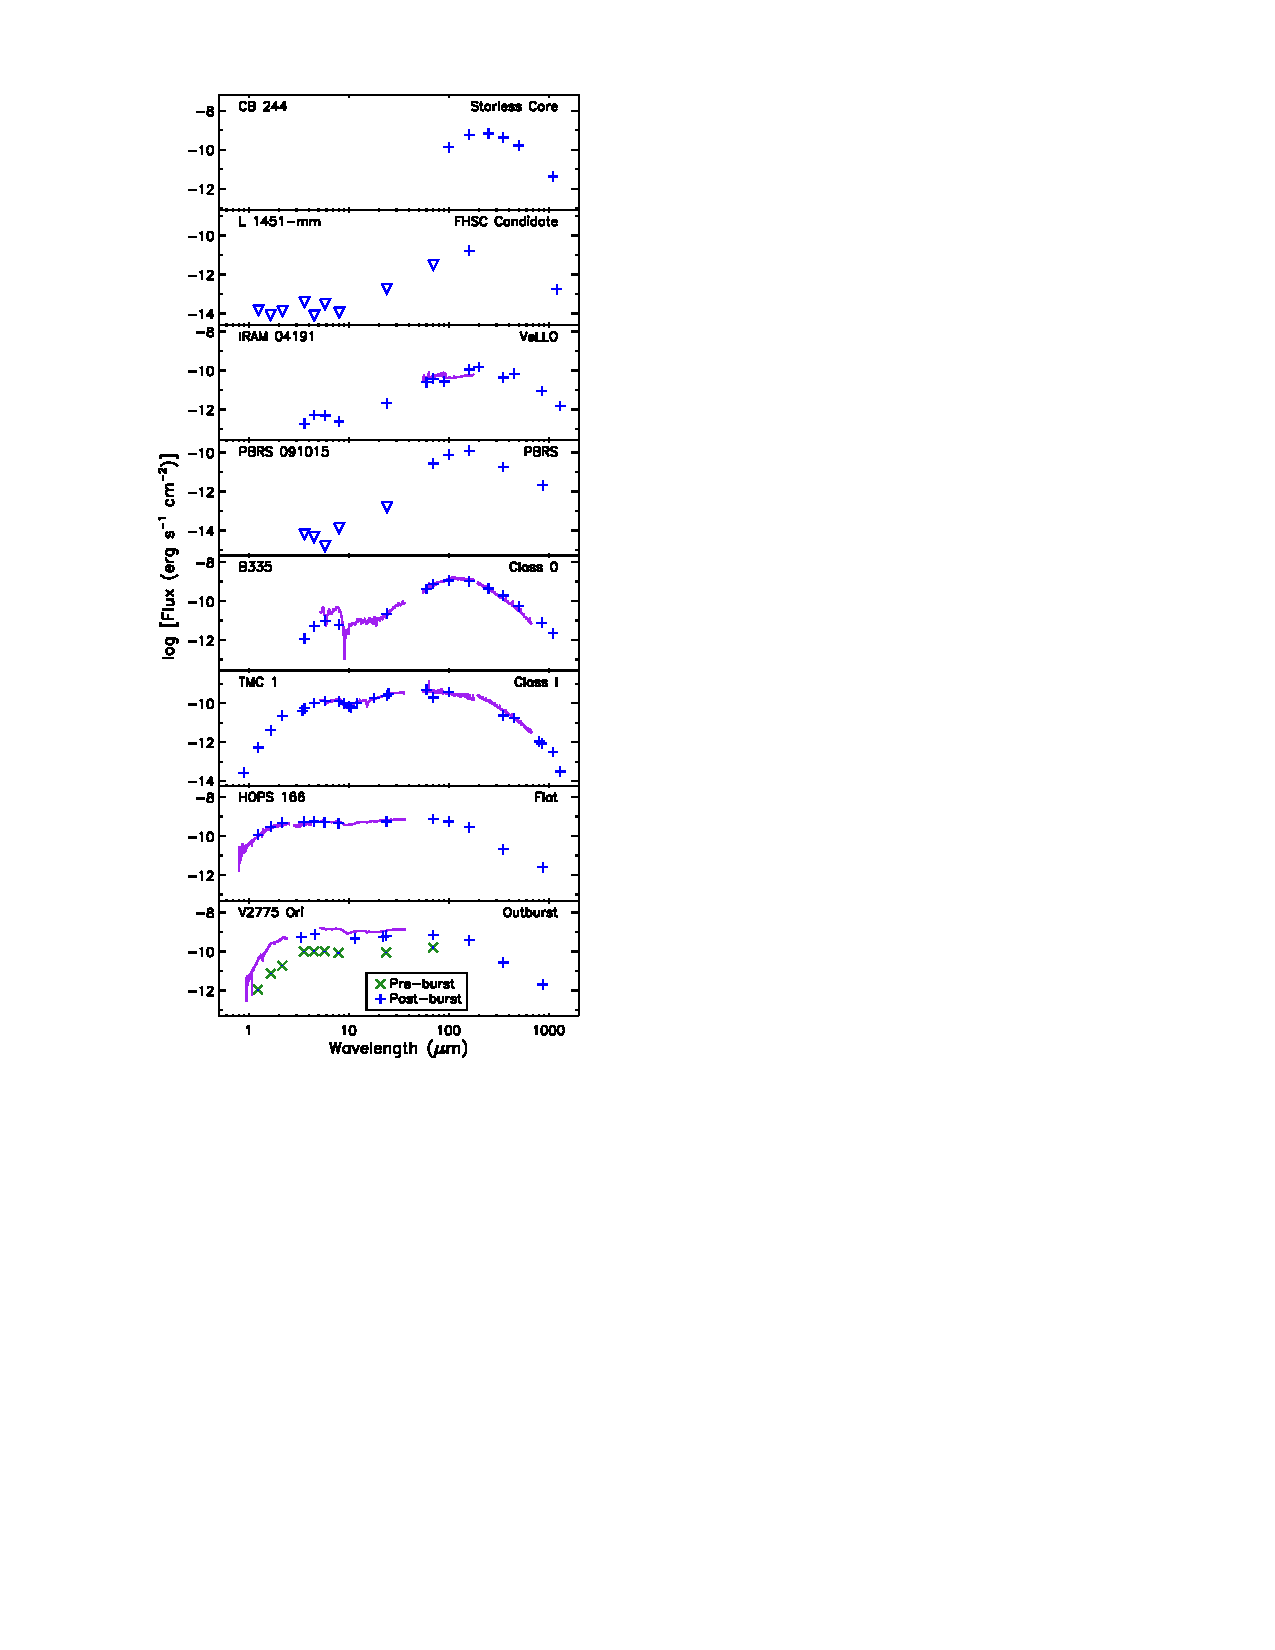
\includegraphics[width=\linewidth]{seds_dunham14}
\caption[Sample SEDs of protostellar cores]{
\label{fig:seds_dunham14}
Sample spectral energy distributions (SEDs) of protostellar cores, together with the assigned class, as collected by \citet{dunham14a}.
}
\end{marginfigure}

These are the earliest indications of star formation we have available to us. We call objects that show one of these signs, and do not fall into one of the other categories, class 0 sources. The dividing line between class 0 and class 1 is that the star begins to heat the dust around it to the point that there is non-trivial infrared emission. Before the advent of \textit{Spitzer} and \textit{Herschel}, the dividing line between class 0 and 1 was taken to be a non-detection in the IR, but as more sensitive IR telescopes became available, the detection limit went down, and it became necessary to specify a dividing line in terms of a luminosity cut. A source is said to be class 0 if more than 0.5\% of its total bolometric output emerges at wavelengths longer than $350$ $\mu$m, i.e., if $L_{\rm smm} / L_{\rm bol} > 0.5\%$, where $L_{\rm smm}$ is defined as the luminosity considering only wavelengths of 350 $\mu$m and longer (Figure \ref{fig:seds_dunham14}).

In practice, measuring $L_{\rm smm}$ can be tricky because it can be hard to get absolute luminosities (as opposed to relative ones) correct in the sub-mm, so it is also common to define the class 0-1 divide in terms of another quantity: the bolometric temperature $T_{\rm bol}$. This is defined as the temperature of a blackbody that has the same flux-weighted mean frequency as the observed spectral energy distribution (SED). That is, if $F_\nu$ is the flux as a function of frequency from the observed source, then we define $T_{\rm bol}$ by the implicit equation
\begin{equation}
\frac{\int \nu B_{\nu}(T_{\rm bol}) \, d\nu}{\int B_{\nu}(T_{\rm bol}) \, d\nu} = \frac{\int \nu F_{\nu}\, d\nu}{\int F_\nu \,d\nu}.
\end{equation}
The class 0-1 dividing line is also sometimes taken to be $T_{\rm bol} = 70$ K. In cases where $L_{\rm smm}$ is accurately measured, $T_{\rm bol}$ is observed to be a reasonably good proxy for $L_{\rm smm} / L_{\rm bol}$ (Figure \ref{fig:tbol_dunham14}).

\begin{marginfigure}
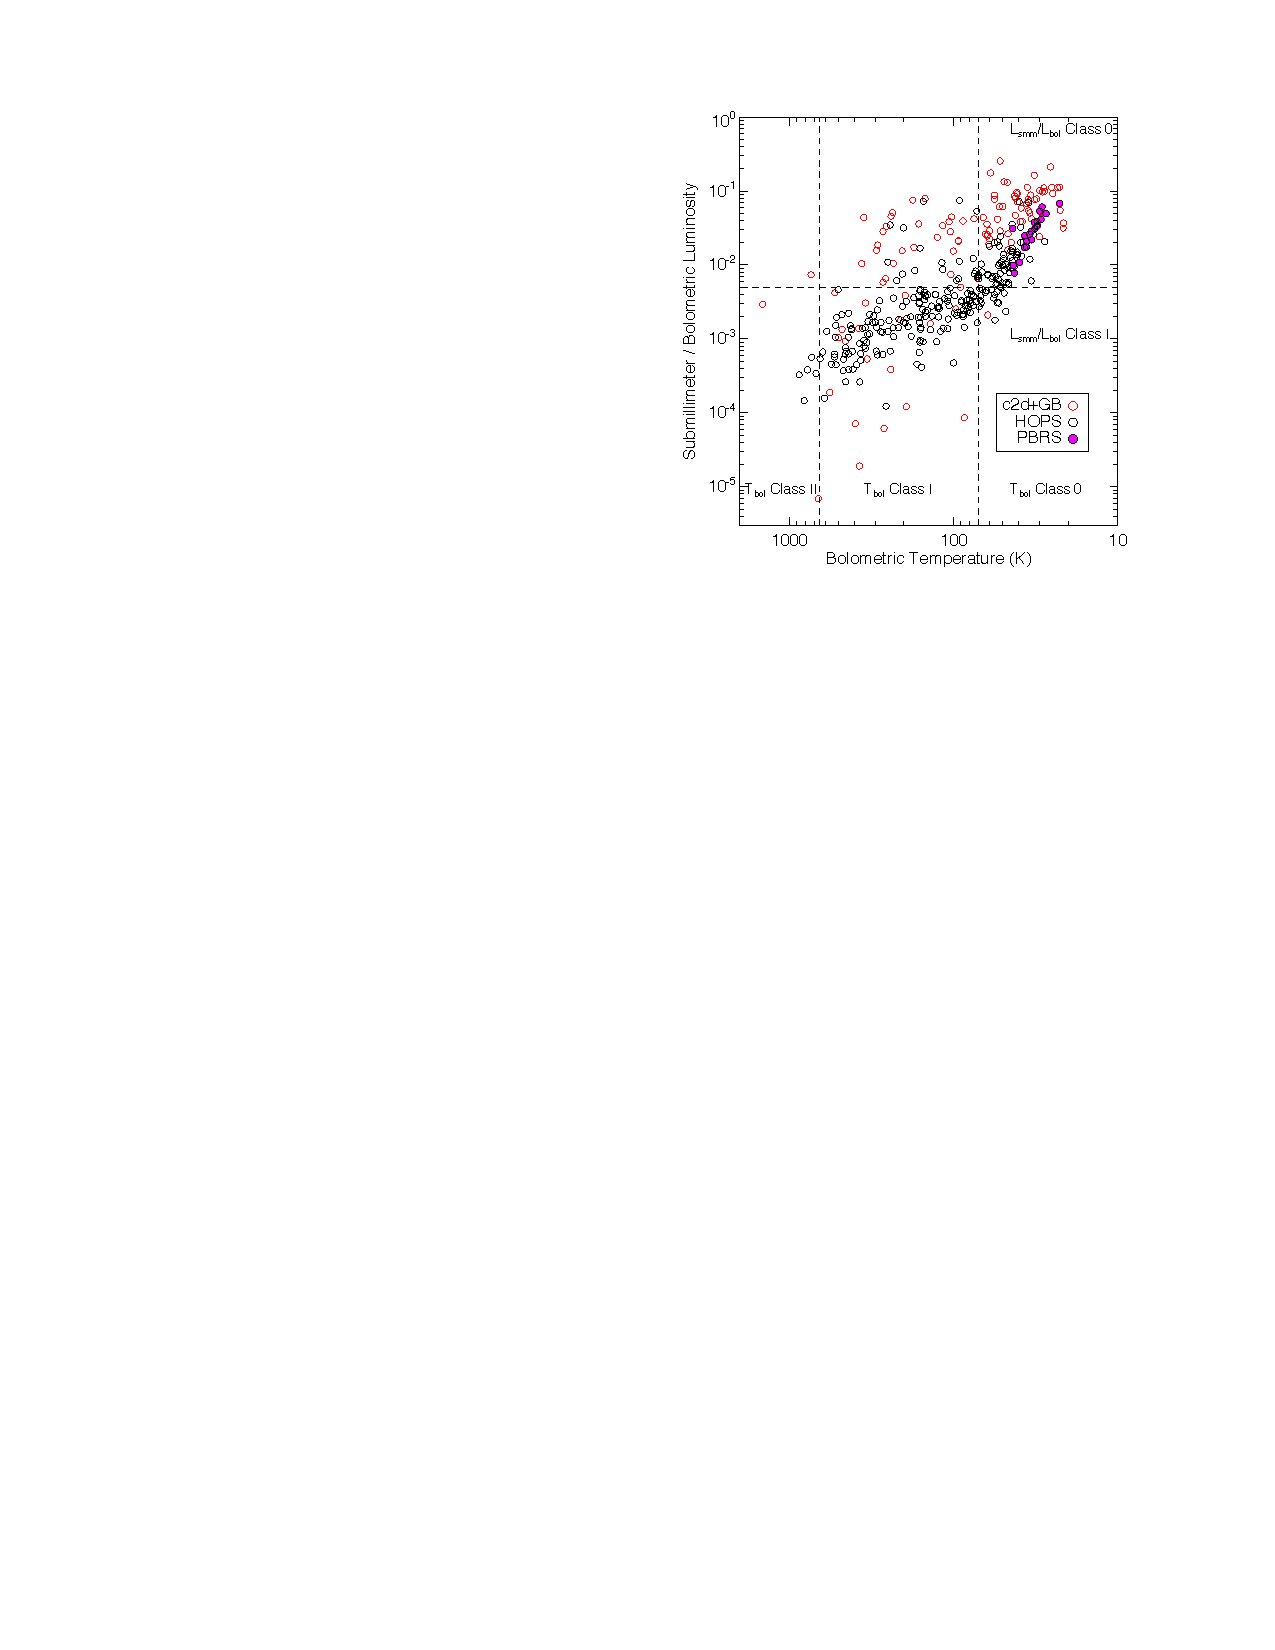
\includegraphics[width=\linewidth]{tbol_dunham14}
\caption[Bolometric temperatures of protostellar cores]{
\label{fig:tbol_dunham14}
Bolometric temperatures of protostellar cores as compared to sub-mm to bolometric luminosity ratios \citep{dunham14a}. The samples shown are from three different surveys as indicated in the legend.
}
\end{marginfigure}

Once protostars reach class I, their evolution into further classes is defined in terms of the infrared spectral energy distribution. The motivating cartoon is a follows. At early times, the envelope of dust around the protostar is very optically thick at visible and even near infrared wavelengths. As a result, we cannot directly observe the stellar photosphere. All the radiation is absorbed by the envelope. The dust is in thermal equilibrium, so it re-radiates that energy. Since the radius of the sphere of dust is much larger than that of the star, and the luminosity radiated by the dust must ultimately be equal to that of the star, this emission must be at lower temperature and thus longer wavelengths. Thus as the radiation propagates outward through the dust it is shifted to longer and longer wavelengths. However, at wavelengths longer than the characteristic sizes of the dust grains, the opacity decreases as roughly $\kappa_\lambda \propto \lambda^{-2}$. Thus eventually the radiation is shifted to wavelengths where the remaining dust is optically thin, and it escapes. What we observe is therefore not a stellar photosphere, but a "dust photosphere".

Given this picture, the greater the column density of the dust around the star, the further it will have to diffuse in wavelength in order to escape. Thus the wavelength at which the emission peaks, or, roughly equivalently, the slope of the spectrum at a fixed wavelength, is a good diagnostic for the amount of circumstellar dust. Objects whose SEDs peak closer to the visible are presumed to be more evolved, because they have lost more of their envelopes.

More formally, this classification scheme was based on fluxes as measured by the \textit{Infrared Astronomical Satellite (IRAS)}. We define
\begin{equation}
\alpha_{\rm IR} = \frac{d\log (\lambda F_{\lambda})}{d\log\lambda},
\end{equation}
as the infrared spectral index, and in practice we measure $\alpha_{\rm IR}$ using two points from the \textit{IRAS} SED: 2.2 $\mu$m and $10-25$ $\mu$m. More positive values of $\alpha_{\rm IR}$ indicate SEDs that peak at longer wavelengths, further into the IR, while more negative values indicate SEDs that peak closer to visible. We define sources with $\alpha_{\rm IR}\geq 0.0$, i.e., rising at longer wavelengths from 2 to 25 $\mu$m, as class I sources. Alternately, in terms of bolometric temperature, the class I to class II transition is generally taken to be at 650 K (Figure \ref{fig:seds_dunham14}).

As more of the envelope accretes, it eventually becomes optically thin at the peak emitting wavelengths of the stellar photosphere. In this case we see the stellar blackbody spectrum, but there is also excess infrared emission coming from the disk of warm, dusty gas that still surrounds the star. Thus the SED looks like a stellar blackbody plus some extra emission at near- or mid-infrared wavelengths. Stars in this class are also know as classical T Tauri stars, named for the first object of the class, although the observational definition of a T Tauri star is somewhat different than the IR classification scheme\footnote{T Tauri stars were first identified in the optical, long before the availability of infrared SEDs. They are defined by high levels of optical variability and the presence of strong chromospheric lines, indicating large amounts of circumstellar material. T Tauri stars are discussed further in Chapter \ref{ch:late_disk}.}, so the alignment may not be perfect. In terms of $\alpha_{\rm IR}$, these stars have indices in the range $-1.6 < \alpha_{\rm IR} < 0$.\footnote{Depending on the author, the breakpoint may  be placed at $-1.5$ instead of $-1.6$. Some authors also introduce an intermediate classification between 0 and I, called flat spectrum sources, which they take to be $-0.3 < \alpha_{\rm IR} < 0.3$.} A slope of around $-1.6$ is what we expect for a bare stellar photosphere without any excess infrared emission coming from circumstellar material. Since the class II phase is the last one during which there is a disk of any significant mass, this is also presumably the phase where planet formation must occur.

The final stages is class III, the category into which we places sources whose SEDs have $\alpha_{\rm IR} < -1.6$. Stars in this class correspond to weak line T Tauri stars. The SEDs of these stars look like bare stellar photospheres in the optical through the mid-infrared. If there is any IR excess at all, it is in the very far IR, indicating that the emitting circumstellar material is cool and located far from the star. The idea here is that the disk around them has begun to dissipate, and is either now optically thin at IR wavelengths or completely dissipated, so there is no strong IR excess. 

However, these stars are still not mature main sequence stars. First of all, their temperatures and luminosities do not correspond to those of main sequence stars. Instead, they are still puffed up to larger radii, so they tend to have either lower effective temperatures or higher bolometric luminosities (or both) than main sequence stars of the same mass. Second, they show extremely high levels of magnetic activity compared to main sequence stars, producing high levels of X-ray emission. Third, they show lithium absorption lines in their atmospheres. This is significant because lithium is easily destroyed by nuclear reactions at high temperatures, and no main sequence stars with convective photospheres show Li absorption. Young stars show it only because there has not yet been time for all the Li to burn.

\section{Statistics of Resolved Stellar Populations}

Young stars tend to be born in the presence of other stars, rather than by themselves. This is not surprising: the gas cores from which they form are very small fragments, $\sim 1$ $\msun$, inside much larger, $\sim 10^6$ $\msun$ clouds. It would be surprising if only one tiny fragment containing $\sim 10^{-6}$ of the total cloud mass were to collapse. We now pull back to somewhat larger scales to look at the formation of stars in groups.

\subsection{Multiplicity}

The smallest scale we can look at beyond a single star is multiple systems. When we do so, we find that a significant fraction of stars are members of multiple systems -- usually binaries, but also some triples, quadruples, and larger. The multiplicity is a strong function of stellar mass. The vast majority of B and earlier stars are multiples, while the majority of G, K, and M stars are singles. This means that most stars are single, but that most massive stars are multiples. The distribution of binary periods is extremely broad, ranging from hours to Myr. The origin of the distribution of periods, and of the mass-dependence of the multiplicity fraction, is a significant area of research in star formation theory, one to which we will return in Chapters \ref{ch:imf_obs}, \ref{ch:imf_th}, and \ref{ch:massivestar}.

\subsection{The Initial Mass Function}

If we observe a cluster of stars, the simplest thing to do is simply count up how many of them there are as a function of mass. The result is one of the most important objects in astrophysics, the initial mass function (IMF). This requires a bit of modeling, since of course what we can actually measure is a luminosity function, not a mass function. The problem of determining the IMF can be tackled in two ways: either by looking at stars in the solar neighborhood, or by looking at individual star clusters.

Looking at stars in the Solar neighborhood has the advantage that there are a lot of them compared to what you see in a clusters, so one gets a lot of statistical power. One also does not have to worry about two things that a major headache for studies of young clusters. First, young clusters usually have remaining bits of gas and dust around them, and this creates reddening that can vary with position and has to be modeled. Second, for clusters younger than $\sim 10$ Myr, the stars are not on the main sequence yet. Since young stars are brighter than main sequence stars of the same mass, this produces and age-mass degeneracy that you have to break by obtaining more information that just luminosities (usually temperatures or colors), and then making pre-main sequence evolutionary models.\footnote{Protostellar evolution is covered in Chapter \ref{ch:protostar_evol}.}

On the other hand, if we want to talk about the IMF of massive stars, we are largely stuck looking at young clusters. The same is also true for brown dwarfs. Since these fade with time, it is hard to find a large number of them outside of young clusters. An additional advantage of star clusters is that they are to good approximation chemically homogenous, so we need not worry about chemical variations masquerading as mass variations.

A big problem for either method is correction for unresolved binaries, particularly at the low mass end, where the companions of brighter stars are very hard to see. When one does all this, the result is the apparently universal or close-to-universal distribution illustrated in Figure \ref{fig:imf_observed}.\footnote{There have been recent claims of IMF variation from extragalactic observation, which we will discuss in Chapter \ref{ch:imf_obs}.} The basic features we see are a break peak centered around a few tenths of $\msun$, with a fairly steep fall off at higher masses that is well fit by a powerlaw function with a slope near $-2.3$. There is also a fall-off at lower masses, although some authors argue for a second peak in the brown dwarf regime. This is a difficult observational problem, both because brown dwarfs are hard to find, and because their evolutionary tracks are less secure than those for more massive stars.

\begin{figure}
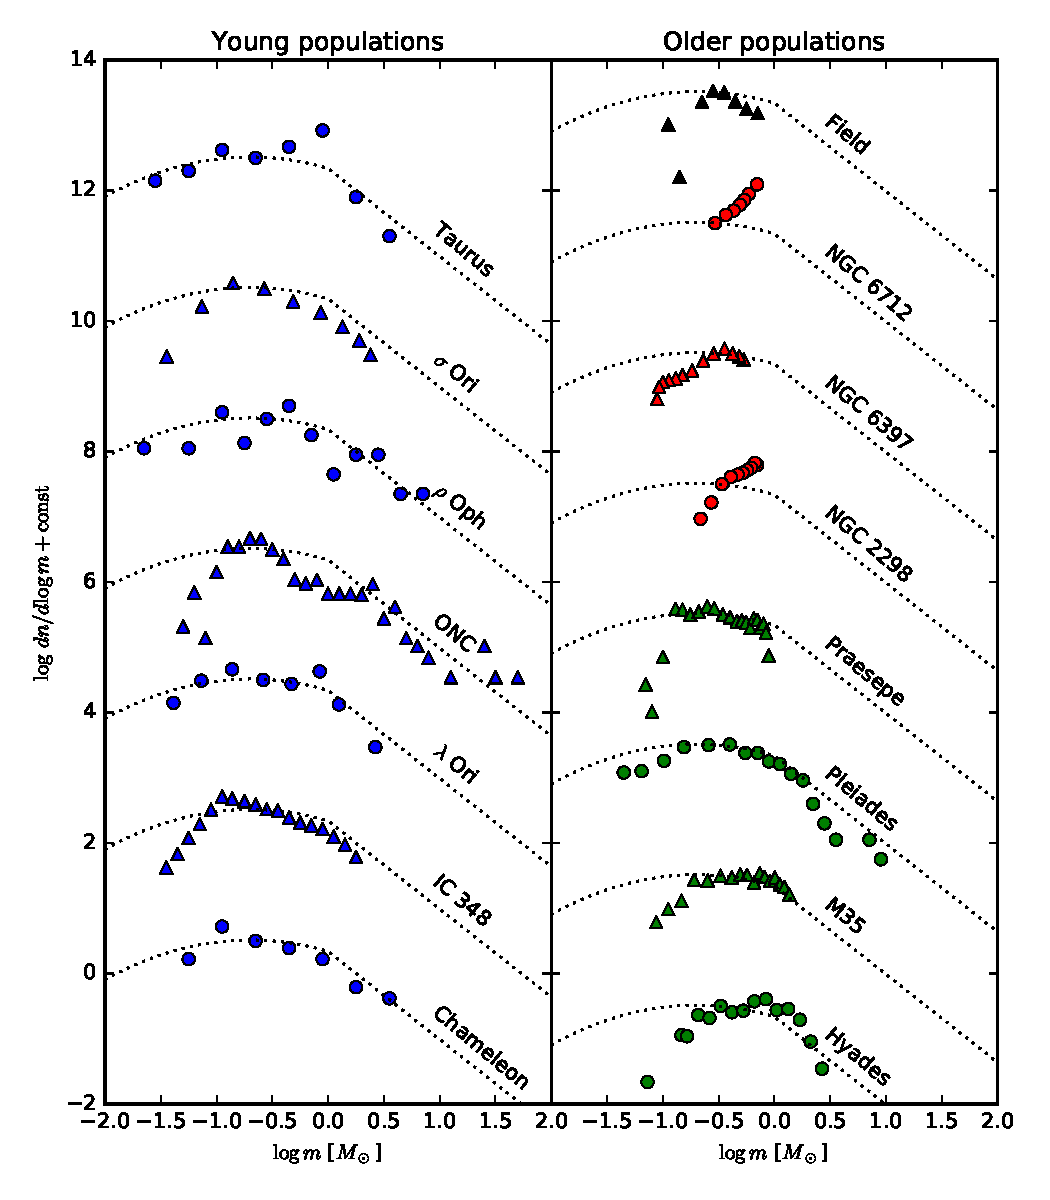
\includegraphics[width=\linewidth]{imf_observed}
\caption[Measured stellar IMFs in a variety of regions]{
\label{fig:imf_observed}
Stellar initial mass functions inferred for a wide variety of regions in the Milky Way (data compilation from \citealt{bastian10a}). The left panel shows young stellar populations (age under $\sim 5$ Myr), while the right panel shows older stellar populations in open clusters (green), globular clusters (red), and the Galactic field (black). The names of the regions are as indicated. The dotted black lines show the \citet{chabrier05a} fit to the IMF (equation \ref{eq:chabrier}). Note that vertical offsets in the plot are arbitrary, and the black dotted lines have been normalized to match the data at $m=0.5$ $M_\odot$. Finally, note that for many regions the data become incomplete below $\sim 0.2$ $M_\odot$.
}
\end{figure}

The functional form shown in Figure \ref{fig:imf_observed} has been parameterized in a number of ways. Two of the most popular are from \citet{kroupa01a, kroupa02c} and \citet{chabrier03a, chabrier05a}.\footnote{See the reviews by \citet{bastian10a} and \citet{offner14a} for a thorough listing of alternate parameterizations.}  Both of these fit the field star data, and the data individual clusters, within the error bars. The functional form for Chabrier is
\begin{equation}
\label{eq:chabrier}
\frac{dn}{d\log m} \propto 
\left\{
\begin{array}{ll}
\exp\left[-\frac{(\log m-\log 0.22)^2}{2\times 0.57^2}\right], &
m<1 \\
\exp\left[-\frac{(-\log 0.22)^2}{2\times 0.57^2}\right] m^{-1.35}, &
m\ge 1
\end{array}
\right.,
\end{equation}
while the functional form for Kroupa is
\begin{equation}
\label{eq:kroupa}
\frac{dn}{d\log m} \propto
\left\{
\begin{array}{ll}
\left(\frac{m}{m_0}\right)^{-\alpha_0}, & m_0 < m < m_1\\
\left(\frac{m_1}{m_0}\right)^{-\alpha_0} \left(\frac{m}{m_1}\right)^{-\alpha_1}, &
m_1 < m < m_2 \\
\left[\prod_{i=1}^{n} \left(\frac{m_i}{m_{i-1}}\right)^{-\alpha_{i-1}}\right] \left(\frac{m}{m_n}\right)^{-\alpha_n}, &
m_{n} < m < m_{n+1}
\end{array}
\right.,
\end{equation}
with
\begin{equation}
\begin{array}{ll}
\alpha_0 = -0.7\pm 0.7, & m_0 = 0.01 \\
\alpha_1 = 0.3\pm 0.5, & m_1 = 0.08 \\
\alpha_2 = 1.3\pm 0.3, & m_2 = 0.5 \\
\alpha_3 = 1.3\pm 0.7, & m_3 = 1,~m_4 \to \infty \\
\end{array}.
\end{equation}
In both of the above expressions, $m$ is understood to be in units of $M_\odot$.

\section{Unresolved Stellar Populations and Extragalactic Star Formation}

What about cases where we cannot resolve the stellar population, as is usually the case for extragalactic work? What can we learn about star formation in that case? The answer turns out to be that the thing we can most directly measure is the star formation rate, and that doing so yields some very interesting results.

\subsection{Measuring the Star Formation Rate: General Theory}

The most basic problem in working with unresolved stellar populations is how we distinguish young stars from main sequence ones. Except for the brightest stars in the nearest galaxies, we cannot obtain spectra, or even colors, for individual stars as we can in the Milky Way. Instead, the strategy we use to isolate young stars is to exploit the fact that massive stars have short lifetimes, so if we measure the total number of massive stars in a galaxy, or some patch of a galaxy, then we are effectively measuring we many such stars formed there over some relatively short period. We can formalize this theory a bit as follows.

Consider stars born with an initial mass function $dn/dm$. The mean stellar mass for this IMF is $\overline{m} = \int dm\, m(dn/dm)$. A time $t$ after a star is born, the star has a luminosity $L(m,t)$, where the luminosity can be bolometric, or integrated over some particular filter or wavelength range. First consider the simplest possible case, a population of stars all born at the same instant at time $0$. A time $t$ later, the luminosity of the stars is
\begin{equation}
L(t) = N_* \int_0^{\infty} dm\, L(m,t) \frac{dn}{dm},
\end{equation}
where $N_*$ is the total number of stars, and we have normalized the IMF so that $\int (dn/dm) \, dm = 1$. That is, we simply integrate the luminosity per star at time $t$ over the mass distribution of stars. Now consider a region, e.g., a galaxy, forming stars at a rate $\dot{M}_*(t)$; in terms of number, the star formation rate is $\dot{N}_*(t) = \dot{M}_*(t)/\overline{m}$. To find the luminosity of the stellar population that is present today, we simply take the expression we just derived and integrate over all the possible stellar ages. Thus we have
\begin{equation}
L =  \int_{0}^\infty dt\, \frac{\dot{M}_*(t)}{\overline{m}}  \int_0^{\infty} dm\, L(m,t) \frac{dn}{dm}.
\end{equation}

By itself this is of limited use, because the right hand side depends on the full star formation history $\dot{M}_*(t)$. However, let us assume that $\dot{M}_*$ is constant in time. The integral still converges as long as $L(m,t)$ reaches 0 after a finite time. In this case the integrals over $m$ and $t$ are separable, and we can rearrange them to
\begin{equation}
\label{eq:sfrtol}
L = \frac{\dot{M}_*}{\overline{m}} \int_0^{\infty} dm \, \frac{dn}{dm} \int_0^\infty dt \, L(m,t) \equiv \frac{\dot{M}_*}{\overline{m}} \int_0^{\infty} dm \, \frac{dn}{dm} \langle L t_{\rm life} \rangle_m 
\end{equation}
In the final step we defined a new quantity $\langle L t_{\rm life} \rangle_m$, which has a simple physical meaning: it is the total amount of radiant energy that a star of mass $m$ puts out over its lifetime.

Notice the expression on the right depends only on the constant star formation rate $\dot{M}_*$, the energy output $\langle L t_{\rm life}\rangle_m$, which we can generally calculate from stellar structure and evolution theory, and the IMF $dn/dm$. Thus if we measure $L$ and use the "known" values of  $\langle L t_{\rm life}\rangle_m$ and $dn/dm$, we can measure the star formation rate. The underlying physical assumption is that the stellar population being observed is in statistical equilibrium between new stars forming and old stars dying, so the total number of stars present and contributing to the light at any time is proportional to the rate at which they are forming. Thus a measurement of the light tells us about the star formation rate.

Is our assumption that $\dot{M}_*$ is constant reasonable? That depends on the system we are observing. For an entire galaxy that is forming stars quiescently and has not been externally perturbed, it is probably reasonable to assume that $\dot{M}_*$ cannot vary on timescales much shorter than the dynamical time of the galaxy, which is $\sim 200$ Myr for a galaxy like the Milky Way. If we choose to observe the luminosity at a wavelength where the light is coming mostly from stars with lifetimes shorter than this, so that $L(m,t)$ reaches 0 (at least to good approximation) at times much less than 200 Myr, then assuming constant $\dot{M}_*$ is quite reasonable.

However, it is always important to keep this constraint in mind -- we can only measure the star formation rate as long as we believe it to be constant on timescales long compared to the lifetimes of the stars responsible for generating the luminosity we are measuring. One can actually see how the ratio of luminosity to star formation rate behaves in systems that do not satisfy the constraint by generating synthetic stellar populations. In the simple case of a system that begins with no stars and then forms star stars at a constant rate, the bolometric luminosity after the onset of star formation just increases linearly with time until the first stars star evolving off the main sequence, and only becomes constant after $\sim 4$ Myr (Figure \ref{fig:lvst_krumholz07}).

\begin{marginfigure}
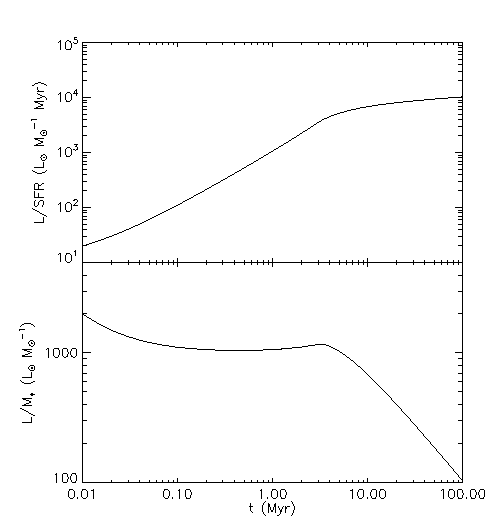
\includegraphics[width=\linewidth]{lvst_krumholz07}
\caption[Bolometric luminosity versus stellar population age]{
\label{fig:lvst_krumholz07}
Bolometric luminosity versus time for stellar populations as a function of population age. The top panel shows the luminosity normalized by the star formation rate, while the bottom shows the luminosity normalized by the total stellar mass. Credit: \citet{krumholz07e}, \copyright\,AAS. Reproduced with permission.
}
\end{marginfigure}

The need to satisfy this constraint generally drives us to look for luminosities that are dominated by very massive stars, because these have very short lifetimes. Thus we will begin by discussing what luminosities we can measure that are particularly good at picking out massive stars. This is far from an exhaustive list -- astronomers have invented many, many methods to infer star formation rates for galaxies at a range of redshifts. The accuracy of these techniques is highly variable, and in some cases amounts to little more than a purely empirical calibration. We focus here on the most reliable and widely used techniques that we can apply to relatively nearby galaxies.

\subsection{Recombination Lines}

Probably the most common technique, and the only one that can be used from the ground for most galaxies, is hydrogen recombination lines. To illustrate why this is useful, it is helpful to look at some galaxy spectra (Figure \ref{fig:spectra_kennicutt92}). As we move from quiescent E4 and SB galaxies to actively star-forming Sc and Sm/Im galaxies, there is a striking different in the prominence of emission lines.

\begin{figure}
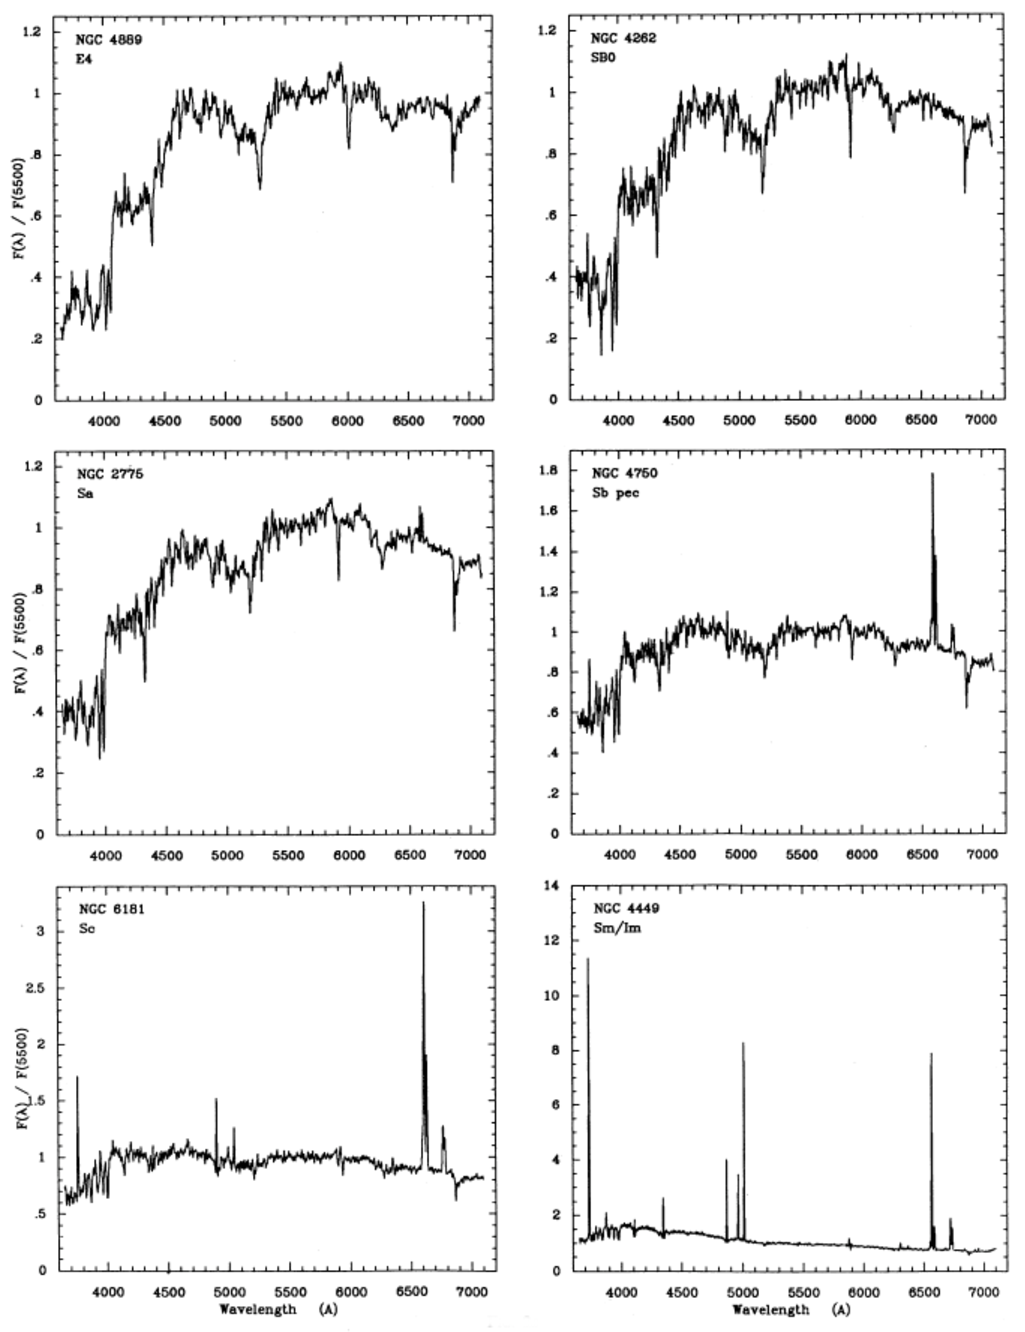
\includegraphics[width=\linewidth]{spectra_kennicutt92}
\caption[Optical spectra of galaxies across the Hubble sequence]{
\label{fig:spectra_kennicutt92}
Example spectra of galaxies of varying Hubble type. In each panel, the galaxy name and Hubble type are listed. Credit: \citet{kennicutt92a}, \copyright\,AAS. Reproduced with permission.
}
\end{figure}

In the example optical spectra, the most prominent lines are the H$\alpha$ line at 6563 \AA\ and the H$\beta$ at 4861 \AA. These are lines produced by the $3\rightarrow 2$ and $4\rightarrow 2$, respectively, electronic transitions in hydrogen atoms. In the infrared (not shown in the figure) are the Paschen $\alpha$ and $\beta$ lines at 1.87 and 1.28 $\mu$m, and the Bracket $\alpha$ and $\gamma$ lines at 4.05 and 2.17 $\mu$m. These come from the $4\rightarrow 3$, $5\rightarrow 3$, $5\rightarrow 4$, and $7\rightarrow 4$ transitions.

Why are these related to star formation? The reason is that these lines come from H~\textsc{ii} regions: regions of ionized gas produced primarily by the ionizing radiation of young stars. Since only massive stars (lager than $10-20$ $\msun$) produce significant ionizing fluxes, these lines indicate the presence of young stars. Within these ionized regions, one gets hydrogen line emission because atoms sometimes recombine to excited states rather than to the ground state. These excited atoms then radiatively decay down to the ground state, producing line emission in the process.

Obtaining a numerical conversion between the observed luminosity in one of these lines and the star formation rate is a four-step process. First, one performs a quantum statistical mechanics calculation to compute the yield of photons in the various lines per recombination. This can be done very precisely from first principles. Second, one equates the total recombination rate to the total ionization rate, and uses this to determine the total rate of emission for the line in question per ionizing photon injected into the nebula. Third, one uses stellar models to compute $\langle L_{\rm ion} t_{\rm life}\rangle_m$, the total ionizing photon production by a star of mass $m$ over its lifetime. Four, one evaluates the integral over the IMF given by equation (\ref{eq:sfrtol}) to obtain the numerical conversion between star formation rate and luminosity. As of this writing, the most up-to-date resource for the results of such calculations is \citet{kennicutt12a}.

Note that there are significant uncertainties in these numbers, the dominant one of which is the IMF. The reason the IMF matters so much is that the light is completely dominated by the massive stars, while the mass is all in the low mass stars that are not observed directly. To give an example, for a Chabrier IMF at zero age, stars more massive than 15 $\msun$ contribute 99\% of the total ionizing flux for a stellar population, but constitute less than 0.3\% of the mass. Thus we are extrapolating by at least a factor of 30 in mass, and small changes in the IMF can produce large changes in the resulting ionizing luminosity to mass conversion.

Another complication is that some of the line emission is likely to be absorbed by dust grains within the source galaxy, and some of the ionizing photons are absorbed by dust grains rather than hydrogen atoms. Thus, one must make an extinction correction to the luminosities.

\subsection{Radio Free-Free}

A closely related method for measuring massive stars is to use free-free emission at radio wavelengths. An H~\textsc{ii} region emits optical lines from transitions between energy levels of hydrogen and other atoms, but it also emits free-free radiation in the radio. This is radiation produced by bremsstrahlung: free electrons scattering off ions, and emitting because accelerating charges emit. It is the opposite side of the coin from recombination line emission: the former occurs when free electrons and protons encounter one another and do not become bound, while the latter occurs when they do.

We will not treat bremsstrahlung or its application to H~\textsc{ii} regions here, but the relevant point for us is that the free-free luminosity of H~\textsc{ii} regions at radio wavelengths is proportional to $n_e n_i$, i.e., the product of the electron and ion densities. Since the recombination rate is also proportional to $n_e n_{\rm H^+}$, and due to chemical balance the recombination rate must equal the ionization rate, the free-free luminosity is directly proportional to the rate at which ionizing photons are injected into the H~\textsc{ii} region. Thus one can convert between free-free emission rate and ionization rate based on the physics of H~\textsc{ii} regions, and from then convert that into a star formation rate exactly as for optical recombination lines.

The free-free method has one major advantage, which is that radio emission is not obscured by dust, so one of the dust absorption corrections goes away. The correction for absorption of ionizing photons by dust grains within the H~\textsc{ii} region remains, but this is generally only a few tens of percent. Thus radio free-free measurements are more reliable that recombination line ones. Indeed, they are the only technique we can use for most H~\textsc{ii} regions in the Milky Way, since these tend to be located in the Galactic plane and thus suffer from heavy extinction at optical wavelengths. The downside is that the free-free emission is quite weak, and separating free-free from other sources of radio emission requires the ability to resolve individual H~\textsc{ii} regions. Thus at present this technique is useful primarily for the Milky Way and a few other nearby galaxies, since those are the only places where we can detect and resolve individual H~\textsc{ii} regions.

\subsection{Infrared}

The recombination line methods work well for galaxies that are like the Milky Way, but considerably less well for galaxies that are dustier and have higher star formation rates. This is because the dust extinction problem becomes severe, so that the vast majority of the Balmer line emission is absorbed. The Paschen and Bracket emission is much less sensitive to this, since those lines are in the IR, but even they can be extincted in very dusty galaxies, and they are also much harder to use than H$\alpha$ and H$\beta$ because they are $1-2$ orders of magnitude less bright intrinsically.

Instead, for dusty sources the tracer of choice is far infrared. The idea here is that, in a sufficiently dusty galaxy, essentially all stellar light will eventually be absorbed by dust grains. These grains will then re-emit the light in the infrared. As a result, the SED peaks in the IR. In this case one can simply use the total IR output of the galaxy as a sort of calorimeter, measuring the total bolometric power of the stars in that galaxy. In galaxies or regions of galaxies with high star formation rates, which tend to be where H$\alpha$ and other recombination line techniques fail, this bolometric power tends to be completely dominated by young stars. Since these stars die quickly, the total number present at any given time is simply proportional to the star formation rate.

The derivation of the conversion in this case is very straightforward -- the $L(m,t)$ that is required is just the total bolometeric output of the stars. Results are given in \citet{kennicutt12a}, and Problem Set 1 includes an example calculation. Of course IR emission has its its problems too. First of all, it misses all the optical and UV radiation from young stars that is not absorbed within the galaxy, which makes it a poor choice for dust-poor galaxies where a majority of the radiation from young stars escapes.

A second problem is that if the SFR is low, then old rather than young stars may dominate the bolometric output. In this case the IR indicator can give an artificially high SFR. A more common problem for the dusty galaxies where IR tends to be used most is contamination from an active galactic nucleus (AGN). If an AGN contributes significantly to the bolometric output of a galaxy, that can masquerade as star formation. This can be hard to detect in a very dusty galaxy where most of the AGN light, along with most of the starlight, is absorbed and reprocessed by dust.

\subsection{Ultraviolet}

Yet another way of measuring star formation rates is by the broadband ultraviolet (UV) flux at wavelengths that are longer than 912 \AA\ (corresponding to 13.6 eV, the energy required to ionized hydrogen) but shorter than where old stars put out most of their light. This range is roughly $1250-2500$ \AA. This light does not ionize hydrogen, so unlike shorter wavelengths it can get out of a galaxy.

For galaxies in the right redshift range this light gets redshifted into the visible, so we can see it from the ground. However, for local galaxies these wavelengths are only accessible from space (or least a balloon or rocket). For this reason this band was not used much until the launch of the \textit{Galaxy Evolution Explorer (GALEX)} satellite, which had detectors operating at 1300-1800 and 1800-2800 \AA (referred to as FUV and NUV, respectively). Emission in the FUV band is dominated by stars with masses $\sim 5$ $\msun$ and up, which have lifetimes of $\sim 50$ Myr, so the total FUV light measures the star formation rate integrated over this time scale. Sadly, \textit{GALEX} is no longer in operation, and there is no comparable mission on the immediate horizon, so this technique is largely of archival value for now.

FUV suffers from the same problems with dust extinction as H$\alpha$, and they are perhaps even more severe, since opacity increases as frequency does. On the other hand, FUV is less sensitive to the IMF than H$\alpha$, because ionizing photons come from hotter and thus more massive stars than FUV ones. For systems with low overall star formation rates, ionization-based star formation rate indicators can become quite noisy due to the rarity of the massive stars they trace. FUV has fewer problems in this regard. However, there is a corresponding disadvantage, in that the $\sim 50$ Myr lifetime of FUV-emitting stars is getting uncomfortably close to the typical orbital periods of galaxies, and so one can legitimately worry about whether the SFR has really be constant over the required timescale. This problem becomes even worse if one looks at small-subregions of galaxies, rather than galaxies as a whole. One also has to worry about stars moving from their birth locations over such long timescales.


\subsection{Combined Estimators}

As one might guess from the discussion thus far, none of the indicators by itself is particularly good. Recombination lines and UV get into trouble in dusty galaxies because they miss light from young stars that is obscured by dust, while IR gets into trouble because it misses light from young stars that is not dust-obscured. This suggests that the best way to proceed is to combine one or more estimators, and this is indeed the current state of the art. A number of combined indicators are suggested in \citet{kennicutt12a}.





\part{Physical Processes}

\chapter{Chemistry and Thermodynamics}
\label{ch:microphysics}

\marginnote{\textbf{Suggested background reading:}
\begin{itemize}
\item \href{http://adsabs.harvard.edu/abs/2014arXiv1402.0867K}{Krumholz, M.~R. 2014, Phys.~Rep., 539, 49}, sections $3.1-3.2$ \nocite{krumholz14c}
\end{itemize}
\textbf{Suggested literature:}
\begin{itemize}
\item \href{http://adsabs.harvard.edu/abs/2010MNRAS.404....2G}{Glover, S.~C.~O., Federrath, C., Mac Low, M.-M., \& Klessen, R.~S. 2010, MNRAS, 404, 2} \nocite{glover10a}
\end{itemize}
}

Having completed our whirlwind tour of the observational phenomenology, we now turn to the physical processes that govern the behavior of the star-forming ISM and its transformation into stars. The goal of this section is to develop physical intuition for how this gas behaves, and to develop some analytic tools for use through the remainder of the book. This chapter covers the microphysics of the cold ISM.

\section{Chemical Processes in the Cold ISM}

We will begin our discussion of the microphysics of the cold ISM with the goal of understanding something important that should be clear from the observational discussion: the parts of the ISM associated with star formation are overwhelmingly molecular gas. This is in contrast to the bulk of the ISM, at least in the Milky Way and similar galaxies, which is composed of atomic or ionized gas with few or no molecules. Our goal is to understand why the ISM in some places becomes predominantly molecular, and how this transition is related star formation. We will focus this discussion on the most important atoms in the ISM: hydrogen, carbon, and oxygen.

\subsection{Hydrogen Chemistry}
\label{ssec:Hchemistry}

Molecular hydrogen is a lower energy state than atomic hydrogen, so an isolated box of hydrogen left for an infinite amount of time will eventually become predominantly molecular. In interstellar space, though, the atomic versus molecular fraction in a gas is determined by a balance between formation and destruction processes.

Atomic hydrogen can turn into molecular hydrogen in the gas phase, but this process is extremely slow. This is ultimately due to the symmetry of the hydrogen molecule. To form an H$_2$ molecule, two H atoms must collide and then undergo a radiative transition that removes enough energy to leave the resulting pair of atoms in a bound state. However, two H atoms that are both in the ground state constitute a symmetric system, as does an H$_2$ molecule in its ground state. Because both the initial and final states are symmetric, the system has no dipole moment, and cannot emit dipole radiation. Thus transitions between the bound and unbound states are forbidden. Radiative transitions can in fact occur, but the rate is extremely small, and generally negligible under astrophysical circumstances.\footnote{One can be more precise about this based on an argument given by \citet{gould63a}. Consider the nuclei fixed, and examine the possible electronic state. The total electronic wave function must be anti-symmetric under particle exchange, so either the spatial part of the wave function must be symmetric and the spin part anti-symmetric, or vice versa. In turns out that the ground, bound state is spatially symmetric and spin anti-symmetric, so the two electrons have opposite spin and the total electronic spin is 0, making the state a singlet; we denote this state $\psi_{\uparrow\downarrow}$. The non-bound repulsive state is the opposite: spatially anti-symmetric, spin symmetric, so the total electronic spin is 1 and the state is a triplet; we denote this $\psi_{\uparrow\uparrow}$. The rate of electric dipole transitions between these two states, and thus the rate at which H$_2$ can form from atomic hydrogen in the gas phase, is proportional to the square of the matrix element $\langle\psi_{\uparrow\uparrow}|\mathbf{D}|\psi_{\uparrow\downarrow}\rangle$, where $\mathbf{D}$ is the electric dipole operator. However, $\mathbf{D}$ does not act on the spin parts of the wave functions, and since the spin parts of $\psi_{\uparrow\downarrow}$ and $\psi_{\uparrow\uparrow}$ are orthogonal, the matrix element should vanish. It does not do so exactly only because spin-spin and spin-orbit interactions slightly perturb the system so that the ground eigenstate is not exactly the pure singlet $\psi_{\uparrow\downarrow}$, but instead is a linear combination of mostly $\psi_{\uparrow\downarrow}$ with a small component of the triplet $\psi_{\uparrow\uparrow}$. The relative size of the triplet component is order the ratio of the spin-orbit and spin-spin interaction energies to the electronic energies, which is $\sim \alpha^2$, where $\alpha \approx 1/137$ is the fine structure constant. Similarly, the repulsive state contains a singlet component of order $\alpha^2$ as well. Thus the bound and repulsive states are not purely orthogonal, but the matrix element is of order $\alpha^2$. Since the transition rate is proportional to the square of this matrix element, it is of order $\alpha^4 \sim 10^{-9}$ compared to allowed transitions.} One can circumvent this limitation by considering either starting or final states there are not symmetric (for example because one of the H atoms is in an excited state, or the final H$_2$ molecule is in an excited state), but this does not lead to a significant rate of gas phase H$_2$ formation either, because the lowest-lying energy states of the H$_2$ molecule are energetic enough that only a negligible fraction of collisions have enough energy to produce them. A third option for gas phase formation is to have three-way collisions, and we will return to this in Chapter \ref{ch:first_stars}. For now we simply remark that, since three-body collisions occur at a rate that depends on the cube of density, at typical interstellar densities they are generally negligible as well.

Due to this limitation, the dominant formation process is instead formation on the surfaces of dust grains. In this case the excess energy released by forming the molecule is transferred into vibrations in the dust grain lattice, and there is no need for forbidden photon emission. The rate of H$_2$ formation by surface catalysis is given by
\begin{equation}
\frac{1}{2} S(T,T_{\rm gr}) \eta(T_{\rm gr}) n_{\rm gr} n_H \sigma_{\rm gr} v_H.
\end{equation}
Here $S$ is the probability that a hydrogen molecule that hits a dust grain will stick, which is a function of both the gas temperature and the grain temperature. $\eta$ is the probability that a grain which sticks will migrate across the grain surface and find another H atom before it is evaporated off the grain surface $n_{\rm gr}$ and $n_H$ are the number densities of grains and hydrogen atoms, $\sigma_{\rm gr}$ is the mean cross section for a dust grain, and $v_H$ is the thermal velocity of the hydrogen atoms.

The last three factors can be estimated reasonably well from observations of dust extinction and gas velocity dispersions, while the former two have to be determined by laboratory measurements and/or theoretical chemistry calculations. Rather than dive into this extensive literature, we will simply skip directly to the result: for conditions appropriate to cool atomic or molecular regions in the Milky Way, the formation rate is roughly
\begin{equation}
\mathcal{R} n n_{\rm H},
\end{equation}
where $n_H$ and $n$ are the number densities of H atoms and H nuclei (in atomic or molecular form), respectively, and $\mathcal{R}\approx 3\times 10^{-17}$ cm$^3$ s$^{-1}$ is the rate coefficient. It may be a factor of a few lower in warmer regions where the sticking probability is reduced. This is for Milky Way dust content. If we go to a galaxy with less dust, the rate coefficient will be reduced proportionally.

The reverse process, destruction, is mostly due to photo-destruction. As with H$_2$ formation, things are somewhat complicated by the symmetry of the H$_2$ system. The binding energy of H$_2$ in the ground state is only 4.5 eV, but this doesn't mean that 4.5 eV photons can destroy it. A reaction of the form
\begin{equation}
{\rm H_2} + h\nu \rightarrow {\rm H}+{\rm H}
\end{equation}
is forbidden by symmetry for exactly the same reason as its inverse, and occurs at a negligibly small rate. Allowed transitions are possible if the H$_2$ molecule is in an excited state that thus asymmetric, or if one of the H atoms is left in an excited state. However, the former is almost never the case at the low temperatures found in molecular clouds, and the latter requires a photon energy of $14.5$ eV. Photons with an energy that high are not generally available, because they can ionize neutral hydrogen and thus have very short mean free paths through the interstellar medium.

Instead, the main H$_2$ destruction process proceeds in two stages. Hydrogen molecules have a series of excited electronic states with energies of $11.2-13.6$ eV (corresponding to $912-1100$ \AA) above the ground state, which produce absorption features known as the Lyman and Werner bands. Since these energies exceed the binding energy of the H$_2$ molecule (4.5 eV), absorptions into them undergo radiative decay to a ground electronic state that can be unbound. This happens roughly 10-15\% of the time, depending on exactly which excited state is decaying. Photons in the LW energy range are produced by hot stars, and the Galaxy is saturated with them, which is why most of the Galaxy's volume is filled with atomic or ionized rather than molecular gas. (There are some galaxies that are mostly molecular, for reasons we will see below.)

Consider a region where the number density of photons of frequency $\nu$ is given by $E^*_{\nu}$. The destruction rate of H$_2$ will then be
\begin{equation}
\int n_{{\rm H}_2} \sigma_{{\rm H}_2,\nu} c E^*_{\nu} f_{{\rm diss,}\nu}\, d\nu,
\end{equation}
where $n_{\rm H_2}$ is the molecular hydrogen number density, $\sigma_{{\rm H}_2,\nu}$ is the absorption cross-section at frequency $\nu$, and $f_{{\rm diss,}\nu}$ is the dissociation probability when a photon of frequency $\nu$ is absorbed. The expression inside the integral is just the number of hydrogen molecule targets times the cross section per target times the number of photons times the relative velocities of the photons and molecules ($=c$) times the probability of dissociation per collision. The integral in frequency goes over the entire LW band, from $912-1100$ \AA.

To understand the circumstances under which H$_2$ can become the dominant form of hydrogen, we can take a simple example. Suppose we have some cloud of gas, which we will treat as a uniform slab, which has a beam of UV radiation shining on its surface. The number density of hydrogen nuclei in the cloud is $n$, and the UV radiation field shining on the surface has a photon number density $E^*_0$. The photon flux is $F^* = c E^*_0$.

As a result of this radiation field, the outer parts of the cloud are atomic hydrogen. However, when a hydrogen molecule absorbs a photon and then re-emits that energy, the energy generally comes out in the form of multiple photons of lower energy, which are no longer able to excite resonant LW transitions. Thus photons are being absorbed as hydrogen forms, and the number of photons penetrating the cloud decreases as one moves further and further into it. Eventually the number of photons drops to near zero, and the gas becomes mostly molecular. This process is known as self-shielding.

We can get a rough estimate of when self-shielding is important by writing down two equations to describe this process. First, let us equate the rates of H$_2$ formation and destruction, i.e., assume the cloud is in chemical equilibrium. (This is generally true because the reaction rates go as $n^2$, so as long as turbulence produces high density regions, there will be places where the reaction occurs quite fast.) This gives
\begin{equation}
\label{eq:chembalance}
n_{\rm H} n \mathcal{R} = \int n_{{\rm H}_2} \sigma_{{\rm H}_2,\nu} c E^*_{\nu} f_{{\rm diss},\nu}\, d\nu
\approx f_{\rm diss}  \int n_{{\rm H}_2} \sigma_{{\rm H}_2,\nu} c E^*_{\nu}\, d\nu.
\end{equation}
In the second step we have made the approximation that $f_{\rm diss}$ is roughly frequency-independent, which is true, since it only varies by factors of less than order unity.

Second, let us write down the equation for photon conservation. This just says that the change in photon number density as we move into the cloud is given by the rate at which collisions with H$_2$ molecules remove photons:
\begin{equation}
\label{eq:dfdx}
\frac{dF^*_{\nu}}{dx}= c \frac{dE^*_{\nu}}{dx} = -n_{H_2} \sigma_{H_2,\nu} c E^*_{\nu}
\end{equation}
In principle there should be a creation term at lower frequencies, representing photons absorbed and re-emitted, but we are only interested in the higher LW frequencies, where there is only photon removal. The term on the right hand side is just the photon absorption rate we calculated above.

Now we can integrate the equation (\ref{eq:dfdx}) over frequency over the LW band. Doing so and dividing by a factor of $c$ gives
\begin{equation}
\frac{dE^*}{dx} = -\int n_{{\rm H}_2} \sigma_{{\rm H}_2,\nu} E^*_{\nu}\, d\nu,
\end{equation}
where $E^*$ is the frequency-integrated photon number density. If we combine this equation with the chemical balance equation (\ref{eq:chembalance}), we obtain
\begin{equation}
\frac{dE^*}{dx} = -\frac{n_{\rm H} n \mathcal{R}}{c f_{\rm diss}}
\end{equation}
This just says that the rate at which photons are taken out of the beam is equal to the recombination rate, increased by a factor of $1/f_{\rm diss}$ because only $\sim 1$ in 10 absorptions actually have to be balanced by a recombination.

If we make the further approximation that the transition from atomic to molecular hydrogen is sharp, so that $n_{\rm H}\approx n$ throughout the atomic layer, and we assume that $\mathcal{R}$ does not vary with position, then the equation is trivial to integrate. At any depth $x$ inside the slab,
\begin{equation}
E^*(x) = E^*_0 - \frac{n^2\mathcal{R}}{c f_{\rm diss}} x.
\end{equation}
The transition to molecular hydrogen occurs where $E^*$ reaches zero, which is at $x_{{\rm H}_2}= c f_{\rm diss} E^*_0 / (n^2 \mathcal{R})$. The total column of atomic hydrogen is
\begin{equation}
N_{\rm H} = nx_{{\rm H}_2} = \frac{c f_{\rm diss} E^*_0}{n\mathcal{R}}
\end{equation}

It is helpful at this point to put in some numbers. In the Milky Way, the observed interstellar UV field is $E^*_0=7.5\times 10^{-4}$ LW photons cm$^{-3}$, and we can take $n=100$ cm$^{-3}$ as a typical number density in a region where molecules might form. Plugging these in with $f_{\rm diss}=0.1$ and $\mathcal{R}=3\times 10^{-17}$ cm$^{-3}$ s$^{-1}$ gives $N_{\rm H} = 7.5\times 10^{20}$, or in terms of mass, a column of $\Sigma=8.4$ $\msun$ pc$^{-2}$. More precise calculations give numbers closer to $2\times 10^{20}$ cm$^{-2}$ for the depth of the shielding layer on one side of a GMC. (Of course a comparable column is required on the other side, too.) Every molecular cloud must be surrounded by an envelope of atomic gas with roughly this column density.

This has important implications. First, this means that molecular clouds with column densities of $100$ $\msun$ pc$^{-2}$ in molecules must have $\sim 10\%$ of their total mass in the form of an atomic shield around them. Second, it explains why most of the Milky Way's ISM in the Solar vicinity is not molecular. In the regions outside of molecular clouds, the mean column density is a bit under $10^{21}$ cm$^{-2}$, so the required shielding column is comparable to the mean column density of the entire atomic disk. Only when the gas clumps together can molecular regions form. This also explains why other galaxies which have higher column densities also have higher molecular fractions. To take an extreme example, the starburst galaxy Arp 220 has a surface density of a few $\times 10^4$ $\msun$ pc$^{-2}$ in its nucleus, and the molecular fraction there is at least 90\%, probably more.

\subsection{Carbon / Oxygen Chemistry}
\label{ssec:cochemistry}

H$_2$ is the dominant species in molecular regions, but it is very hard to observe directly for the reasons discussed in Chapter \ref{ch:obscold} -- the temperatures are too low for it to be excited. Moreover, as we will discuss shortly, H$_2$ is also not the dominant coolant for the same reason. Instead, that role falls to the CO molecule.

Why is CO so important? The main reason is abundances: the most abundant elements in the universe after H and He are O, C, and N, and CO is the simplest (and, under ISM conditions, most energetically favorable) molecule that can be made from them. Moreover, CO can be excited at very low temperatures because its mass is much greater than that of H$_2$, and its dipole moment is weak but non-zero. (A weak dipole moment lowers the energy of radiation emitted, which in turn lowers the temperature needed for excitation.)

Just as in the bulk of the ISM, hydrogen is mostly H, in the bulk of the ISM the oxygen is mostly O and the carbon is mostly C$^+$. It is C$^+$ rather than C because the ionization potential of carbon is less than that of hydrogen, and as a result it tends to be ionized by starlight. So how do we get from C$^+$ and O to CO?

The formation of CO is substantially different than that of H$_2$ in that it is dominated by gas-phase rather than grain-surface reactions. This is because there are no symmetric systems involved, and thus no symmetry barriers to radiation. However, since the temperatures in regions where CO is forming tend to be low, the key processes involve ion-neutral reactions. These are important because the rate at which they occur is to good approximation independent of temperature, while neutral-neutral reactions occur at a rate that declines with temperature as roughly $T^{1/2}$.\footnote{These dependencies are relatively easy to understand. For neutral-neutral reactions, there are no long-distance forces between particles, and thus the rate of collisions is proportional to the mean velocities of the particles involved, which scales as $T^{1/2}$. In contrast, for ion-neutral reactions the ion induces an electric dipole moment in the neutral and then attracts it via Coulomb forces. The slower the particles' relative velocities, the more important is this electric attraction, and this effect cancels out the lower overall rates of encounter caused by lower particle velocities.}

There are two main pathways to CO. One passes through the OH molecule, and involves a reaction chain that looks like
\begin{eqnarray}
{\rm H}_2 + {\rm CR} & \rightarrow & {\rm H}_2^+ + e^{-} + {\rm CR} \\
{\rm H}_2^+ + {\rm H}_2 & \rightarrow & {\rm H}_3^+ + {\rm H} \\
{\rm H}_3^+ + {\rm O} & \rightarrow & {\rm OH}^+ + {\rm H}_2 \\
{\rm OH}^+ + {\rm H}_2 & \rightarrow & {\rm OH}_2^+ + {\rm H} \\
{\rm OH}_2^+ + e^{-} & \rightarrow & {\rm OH} + {\rm H} \\
{\rm C}^+ + {\rm OH} & \rightarrow & {\rm CO}^+ + {\rm H} \\
{\rm CO}^+ + {\rm H}_2 & \rightarrow & {\rm HCO}^+ + {\rm H} \\
{\rm HCO}^+ + e^{-} & \rightarrow & {\rm CO} + {\rm H}.
\end{eqnarray}
Here CR indicates cosmic ray. There are also a number of possible variants (e.g., the OH$_2^+$ could form OH$_3^+$ before proceeding to OH). The second main route is through the CH molecule, where reaction chains tend to follow the general pattern
\begin{eqnarray}
{\rm C}^+ + {\rm H}_2 & \rightarrow & {\rm CH}_2^+ + h\nu \\
{\rm CH}_2^+ + e & \rightarrow & {\rm CH} + {\rm H} \\
{\rm CH} + {\rm O} & \rightarrow & {\rm CO} + {\rm H}.
\end{eqnarray}
The rate at which the first reaction chain manufactures CO is limited by the supply of cosmic rays that initiate the production of H$_2^+$, while the rate at which the second reaction chain proceeds is limited by the rate of the final neutral-neutral reaction. Which chain dominates depends on the cosmic ray ionization rate, density, temperature, and similar details. Note that both of these reaction chains require the presence of H$_2$. 

CO is destroyed via radiative excitation followed by dissociation in essentially the same manner as H$_2$. The shielding process for CO is slightly different however. As with H$_2$, photons that dissociate CO can be absorbed both by dust grains and by CO molecules. However, due to the much lower abundance of CO compared to H$_2$, the balance between these two processes is quite different than it is for hydrogen, with dust shielding generally the more important of the two. Moreover, there is non-trivial overlap between the resonance lines of CO and those of H$_2$, and thus there can be cross-shielding of CO by H$_2$.

At this point the problem is sufficiently complex that one generally resorts to numerical modeling. The net result is that clouds tend to have a layered structure. In poorly-shielded regions where the FUV has not yet been attenuated, H~\textsc{i} and C$^+$ dominate. Further in, where the FUV has been partly attenuated, H$_2$ and C$^+$ dominate. Finally a transition to H$_2$ and CO as the dominant chemical states occurs at the center. For typical Milky Way conditions, the final transition to a CO-dominated composition occurs once the V-band extinction $A_V$ exceeds $1-2$ mag. This corresponds to a column density of a few $\times 10^{21}$ cm$^{-2}$, or $\sim 20$ $\msun$ pc${-2}$, for Milky Way dust. In comparison, recall that typical GMC column densities are $\sim 10^{22}$ cm$^{-2}$, or $\sim 100$ $\msun$ pc$^{-2}$. This means that there is a layer of gas where the hydrogen is mostly H$_2$ and the carbon is still C$^+$, but it constitutes no more than a few tens of percent of the mass. However, in galaxies with lower dust to gas ratios, the layer where H$_2$ dominates but the carbon is not yet mostly CO can be much larger.

\section{Thermodynamics of Molecular Gas}

Having discussed the chemistry of molecular gas, we now turn to the problem of its thermodynamics. What controls the temperature of molecular gas? We have already seen that observations imply temperatures that are extremely low, $\sim 10$ K or even a bit less. How are such cold temperatures achieved? To answer this question, we must investigate what processes heat and cool the molecular ISM.

\subsection{Heating Processes}

The dominant heating process in the atomic ISM is the grain photoelectric effect: photons from stars with energies of $\sim 8-13.6$ eV hit dust grains and eject fast electrons via the photoelectric effect. The fast electrons then thermalize and deposit their energy at heat in the gas. The rate per H nucleus at which this process deposits energy can be written approximately as\footnote{For a justification of this statement, and a much more complete description of the photoelectric heating process, see a general interstellar medium textbook such as \citet{tielens05a} or \citet{draine11a}.}
\begin{equation}
\Gamma_{\rm PE} \approx 4.0\times 10^{-26} \chi_{\rm FUV} Z_d' e^{-\tau_d}\mbox{ erg s}^{-1}
\end{equation}
where $\chi_{\rm FUV}$ is the intensity of the far ultraviolet radiation field scaled to its value in the Solar neighborhood, $Z'_d$ is the dust abundance scaled to the Solar neighborhood value, and $\tau_d$ is the dust optical depth to FUV photons. The result is, not surprisingly, proportional to the radiation field strength (and thus the number of photons available for heating), the dust abundance (and thus the number of targets for those photons), and the $e^{-\tau_d}$ factor by which the radiation field is attenuated.

At FUV wavelengths, typical dust opacities are $\kappa_d \approx 500$ cm$^2$ g$^{-1}$, so at a typical molecular cloud surface density $\Sigma\approx 50 - 100$ M$_\odot$ pc$^{-2}$, $\tau_d \approx 5-10$, and thus $e^{-\tau_d} \approx 10^{-3}$. Thus in the interiors of molecular clouds, photoelectric heating is strongly suppressed simply because the FUV photons cannot get in. Typical photoelectric heating rates are therefore of order a few $\times 10^{-29}$ erg s$^{-1}$ per H atom deep in cloud interiors, though they can obviously be much larger at cloud surfaces or in regions with stronger radiation fields.

We must therefore consider another heating process: cosmic rays. The great advantage of cosmic rays over FUV photons is that, because they are relativistic particles, they have much lower interaction cross sections, and thus are able to penetrate into regions where light cannot. The process of cosmic ray heating works as follows. The first step is the interaction of a cosmic ray with an electron, which knocks the electron off a molecule:
\begin{equation}
\mbox{CR}+\mbox{H}_2 \rightarrow \mbox{H}_2^+ +e^- + \mbox{CR}
\end{equation}
The free electron's energy depends only weakly on the CR's energy, and is typically $\sim 30$ eV.

The electron cannot easily transfer its energy to other particles in the gas directly, because its tiny mass guarantees that most collisions are elastic and transfer no energy to the impacted particle. However, the electron also has enough energy to ionize or dissociate other hydrogen molecules, which provides an inelastic reaction that can convert some of its 30 eV to heat. Secondary ionizations do indeed occur, but in this case almost all the energy goes into ionizing the molecule (15.4 eV), and the resulting electron has the same problem as the first one: it cannot effectively transfer energy to the much more massive protons.

Instead, there are a number of other channels that allow electrons to dump their energy into motion of protons, and the problem is deeply messy. The most up to date work on this is Goldsmith et al.~(2012, ApJ, 756, 157), and we can very briefly summarize it here. A free electron can turn its energy into heat through three channels. The first is dissociation heating, in which the electron strikes an H$_2$ molecule and dissociates it:
\begin{equation}
e^- + {\rm H}_2 \rightarrow 2{\rm H} + e^{-}.
\end{equation}
In this reaction any excess energy in the electron beyond what is needed to dissociate the molecule (4.5 eV) goes into kinetic energy of the two recoiling hydrogen atoms, and the atoms, since they are massive, can then efficiently share that energy with the rest of the gas. A second pathway is that an electron can hit a hydrogen molecule and excite it without dissociating it. The hydrogen molecule then collides with another hydrogen molecule and collisionally de-excites, and the excess energy again goes into recoil, where it is efficiently shared. The reaction is
\begin{eqnarray}
e^- + {\rm H}_2 & \rightarrow & {\rm H}_2^* + e^{-} \\
{\rm H}_2^* + {\rm H}_2 & \rightarrow & 2 {\rm H}_2.
\end{eqnarray}
Finally, there is chemical heating, in which the H$_2^+$ ion that is created by the cosmic ray undergoes chemical reactions with other molecules that release heat. There are a large number of possible exothermic reaction chains, for example
\begin{eqnarray}
{\rm H}_2^+ + {\rm H}_2 & \rightarrow & {\rm H}_3^+ + {\rm H} \\
{\rm H}_3^+ + {\rm CO} & \rightarrow & {\rm HCO}^+ + {\rm H}_2 \\
{\rm HCO}^+ + e^- & \rightarrow & {\rm CO} + {\rm H}.
\end{eqnarray}
Each of these reactions produces heavy ions recoiling at high speed that can efficiently share their energy via collisions. Computing the total energy release requires summing over all these possible reaction chains, which is why the problem is ugly. The final results is that the energy yield per primary cosmic ray ionization is in the range $\sim 13$ eV under typical molecular cloud conditions, but that it can be several eV higher or lower depending on the local density, electron abundance, and similar variables.

Combining this with the primary ionization rate for cosmic rays in the Milky Way, which is observationally-estimated to be about  $\sim 10^{-16}$ s$^{-1}$ per H nucleus in molecular clouds, this gives a total heating rate per H nucleus
\begin{equation}
\Gamma_{\rm CR} \sim 2\times 10^{-27}\mbox{ erg s}^{-1}.
\end{equation}
The heating rate per unit volume is $\Gamma_{\rm CR} n$, where $n$ is the number density of H nuclei ($=2\times$ the density of H molecules). This is sufficient that, in the interiors of molecular clouds, it generally dominates over the photoelectric heating rate.

\subsection{Cooling Processes}

In molecular clouds there are two main cooling processes: molecular lines and dust radiation. Dust can cool the gas efficiently because dust grains are solids, so they are thermal emitters. However, dust is only able to cool the gas if collisions between dust grains and hydrogen molecules occur often enough to keep them thermally well-coupled. Otherwise the grains cool off, but the gas stays hot. The density at which grains and gas become well-coupled is around $10^4-10^5$ cm$^{-3}$, which is higher than the typical density in a GMC, so we will not consider dust cooling further at this point. We will return to it later in Chapters \ref{ch:first_stars} and \ref{ch:protostar_form} when we discuss collapsing objects, where the densities do get high enough for dust cooling to be important.

The remaining cooling process is line emission, and by far the most important molecule for this purpose is CO, for the reasons stated earlier. The physics is fairly simple. CO molecules are excited by inelastic collisions with hydrogen molecules, and such collisions convert kinetic energy to potential energy within the molecule. If the molecule de-excites radiatively, and the resulting photon escapes the cloud, the cloud loses energy and cools.

Let us make a rough attempt to compute the cooling rate via this process. A diatomic molecule like CO can be excited rotationally, vibrationally, or electronically. At the low temperatures found in molecular clouds, usually only the rotational levels are important. These are characterized by an angular momentum quantum number $J$, and each level $J$ has a single allowed radiative transition to level $J-1$. Larger $\Delta J$ transitions are strongly suppressed because they require emission of multiple photons to conserve angular momentum.

Unfortunately the CO cooling rate is quite difficult to calculate, because the lower CO lines are all optically thick. A photon emitted from a CO molecule in the $J=1$ state is likely to be absorbed by another one in the $J=0$ state before it escapes the cloud, and if this happens that emission just moves energy around within the cloud and provides no net cooling. The cooling rate is therefore a complicated function of position within the cloud -- near the surface the photons are much more likely to escape, so the cooling rate is much higher than deep in the interior. The velocity dispersion of the cloud also plays a role, since large velocity dispersions Doppler shift the emission over a wider range of frequencies, reducing the probability that any given photon will be resonantly re-absorbed before escaping.

In practice this means that CO cooling rates usually have to be computed numerically, and will depend on the cloud geometry if we want accuracy to better than a factor of $\sim 2$. However, we can get a rough idea of the cooling rate from some general considerations. The high $J$ levels of CO are optically thin, since there are few CO molecules in the $J-1$ state capable of absorbing them, so photons they emit can escape from anywhere within the cloud. However, the temperatures required to excite these levels are generally high compared to those found in molecular clouds, so there are few molecules in them, and thus the line emission is weak. Moreover, the high $J$ levels also have high critical densities, so they tend to be sub-thermally populated, further weakening the emission.

On other hand, low $J$ levels of CO are the most highly populated, and thus have the highest optical depths. Molecules in these levels produce cooling only if they are within one optical depth the cloud surface. Since this restricts cooling to a small fraction of the cloud volume (typical CO optical depths are many tens for the $1\rightarrow 0$ line), this strongly suppresses cooling.

The net effect of combining the suppression of low $J$ transitions by optical depth effects and of high $J$ transitions by excitation effects is that cooling tends to be dominated a single line produced by the lowest $J$ level for which the line is not optically thick. This line is marginally optically thin, but is kept close to LTE by the interaction of lower levels with the radiation field. Which line this is depends on the column density and velocity dispersion of the cloud, but typical peak $J$ values in Milky Way-like galaxies range from $J=2\rightarrow 1$ to $J=5\rightarrow 4$.

For an optically thin transition of a quantum rotor where the population is in LTE, the rate of energy emission per H nucleus from transitions between angular momentum quantum numbers $J$ and $J-1$ is given by
\begin{eqnarray}
\label{eq:lambdaco}
\Lambda_{J,J-1} & = & x_{\rm em} \frac{(2J+1)e^{-E_J/k_B T}}{Z(T)} A_{J,J-1} (E_J - E_{J-1}) \\
E_J & = & h B J (J+1) \\
A_{J,J-1} & = & \frac{512\pi^4 B^3\mu^2}{3hc^3} \frac{J^4}{2J+1}.
\end{eqnarray}
Here $x_{\rm em}$ is the abundance of the emitting species per H nucleus, $T$ is the gas temperature, $Z(T)$ is the partition function, $A_{J,J-1}$ is the Einstein $A$ coefficient from transitions from state $J$ to state $J-1$, $E_J$ is the energy of state $J$, $B$ is the rotation constant for the emitting molecule, and $\mu$ is the electric dipole moment of the emitting molecule. The first equation is simply the statement that the energy loss rate is given by the abundance of emitters multiplied by the fraction of emitters in the $J$ state in question times the spontaneous emission rate for this state times the energy emitted per transition. Note that there is no explicit density dependence as a result of our assumption that the level with which we are concerned is in LTE. The latter two equations are general results for quantum rotors.

The CO molecule has $B=57$ GHz and $\mu=0.112$ Debye, and at Solar metallicity its abundance in regions where CO dominates the carbon budget is $x_{\rm CO} \approx 1.1\times 10^{-4}$. Plugging in these two values, and evaluating for $J$ in the range $2-5$, typical cooling rates are of order $10^{-27}-10^{-26}$ erg cm$^{-3}$ when the temperature is $\sim 10$ K. This matches the heating rate we computed above, and this is why the equilibrium temperatures of molecular clouds are $\sim 10$ K.

\subsection{Implications}

The calculation we have just performed has two critical implications that strongly affect the dynamics of molecular clouds. First, the temperature will be relatively insensitive to variations in the local heating rate. The cosmic ray and photoelectric heating rates are to good approximation temperature-independent, but the cooling rate is extremely temperature sensitive because, for the dominant cooling lines of CO have level energies are large compared to $k_B T$. Equation (\ref{eq:lambdaco}) would in fact seem to suggest that the cooling rate is exponentially sensitive to temperature. In practice the sensitivity is not quite that great, because which $J$ dominates changes with temperature. Nonetheless, numerical calculations still show that $\Lambda_{\rm CO}$ varies with $T$ to a power of $p \sim 2-3$. This means that a factor $f$ increase in the local heating rate will only change the temperature by a factor $\sim f^{1/p}$. Thus we expect molecular clouds to be pretty close to isothermal, except near extremely strong local heating sources.

A second important point is the timescales involved. The gas thermal energy per H nucleus is\footnote{This equation is only approximate because this neglects quantum mechanical effects that are of order unity at these low temperatures. However, since the result we are after here is an order of magnitude one, we will not worry about this corrections.}
\begin{equation}
e \approx \frac{1}{2}\left(\frac{3}{2}k_B T\right) = 10^{-15} \left(\frac{T}{10\mbox{ K}}\right)\mbox{ erg}
\end{equation}
The factor of $1/2$ comes from 2 H nuclei per H$_2$ molecule. The characteristic cooling time is $t_{\rm cool} = e/\Lambda_{\rm CO}$. Suppose we have gas that is mildly out of equilibrium, say $T=20$ K instead of $T=10$ K. The heating and cooling are far out of balance, so we can ignore heating completely compared to cooling. At a cooling rate of $\Lambda_{\rm CO} \sim \mathrm{few} \times 10^{-26}$ erg s$^{-1}$ for 20 K gas (assuming the scaling $\Lambda_{\rm CO} \propto T^{2-3}$ as mentioned above), $t_{\rm cool} \sim 1$ kyr. In contrast, the crossing time for a molecular cloud is $t_{\rm cr} = L/\sigma \sim 10$ Myr for $L=30$ pc and $\sigma = 3$ km s$^{-1}$. The conclusion of this analysis is that radiative effects happen on time scales {\it much} shorter than mechanical ones. Gas that is driven out of thermal equilibrium by any hydrodynamic effect will return to its equilibrium temperature long before any mechanical motions can take place. For this reason, gas in molecular clouds is often approximated as isothermal.

\chapter{Gas Flows and Turbulence}
\label{ch:turbulence}

\marginnote{\textbf{Suggested background reading:}
\begin{itemize}
\item \href{http://adsabs.harvard.edu/abs/2014arXiv1402.0867K}{Krumholz, M.~R. 2014, Phys.~Rep., 539, 49}, section 3.3 \nocite{krumholz14c}
\end{itemize}
\textbf{Suggested literature:}
\begin{itemize}
\item \href{http://adsabs.harvard.edu/abs/2013MNRAS.436.1245F}{Federrath, C. 2013, MNRAS, 436, 1245} \nocite{federrath13b}
\end{itemize}
}

This chapter covers the physics of turbulence in the cold interstellar medium. This will be something of a whirlwind tour, since turbulence is an entire research discipline unto itself. Our goal is to understand the basic statistical techniques used to describe and model interstellar turbulence, so that we will be prepared to apply them in the context of star formation.

\section{Characteristic Numbers for Fluid Flow}

\subsection{The Conservation Equations}

To understand the origins of turbulence, both in the ISM and more generally, we start by examining the equations of fluid dynamics and the characteristic numbers that they define. Although the ISM is magnetized, we will first start with the simpler case of an unmagnetized fluid. Fluids are governed by a series of conservation laws. The most basic one is conservation of mass:
\begin{equation}
\frac{\partial}{\partial t} \rho = -\nabla \cdot (\rho\mathbf{v}).
\end{equation}
This equation asserts that the change in mass density at a fixed point is equal to minus the divergence of density times velocity at that point. Physically, this is very intuitive: density at a point changes at a rate that is simply equal to the rate at which mass flows into or out of an infinitesimal volume around that point.

We can write a similar equation for conservation of momentum:
\begin{equation}
\label{eq:momentum}
\frac{\partial}{\partial t}(\rho \mathbf{v}) = -\nabla \cdot(\rho \mathbf{v v}) - \nabla P + \rho \nu \nabla^2 \mathbf{v}.
\end{equation}
Note that the term $\mathbf{vv}$ here is a tensor product. This is perhaps more clear if we write things out in index notation:
\begin{equation}
\frac{\partial}{\partial t}(\rho v_i) = -\frac{\partial}{\partial x_j} (\rho v_i v_j) - \frac{\partial}{\partial x_i} P
+ \rho \nu \frac{\partial}{\partial x_j}\left(\frac{\partial}{\partial x_j} v_i\right)
\end{equation}
The intuitive meaning of this equation can be understood by examining the terms one by one. The term $\rho\mathbf{v}$ is the density of momentum at a point. The term $\nabla \cdot(\rho \mathbf{v v})$ is, in analogy to the equivalent term in the conservation of mass equation, the rate at which momentum is advected into or out of that point by the flow. The term $\nabla P$ is the rate at which pressure forces acting on the fluid change its momentum. Finally, the last term, $\rho \nu \nabla^2 \mathbf{v}$, is the rate at which viscosity redistributes momentum; the quantity $\nu$ is called the kinematic viscosity.

The last term, the viscosity one, requires a bit more discussion. All the other terms in the momentum equation are completely analogous to Newton's second law for single particles. The viscous term, on the other hand, is unique to fluids, and does not have an analog for single particles. It describes the change in fluid momentum due to the diffusion of momentum from adjacent fluid elements. We can understand this intuitively: a fluid is composed of particles moving with random velocities in addition to their overall coherent velocity. If we pick a particular fluid element to follow, we will notice that these random velocities cause some of the particles that make it up to diffuse across its boundary to the neighboring element, and some particles from the neighboring element to diffuse into the one we are following. The particles that wander across the boundaries of our fluid element carry momentum with them, and this changes the momentum of the element we are following. The result is that momentum diffuses across the fluid, and this momentum diffusion is called viscosity.

Viscosity is interesting and important because it's the only term in the equation that converts coherent, bulk motion into random, disordered motion. That is to say, the viscosity term is the only one that is dissipative, or that causes the fluid entropy to change. 

\subsection{The Reynolds Number and the Mach Number}
\label{ssec:reynolds_mach}

To understand the relative importance of terms in the momentum equation, it is helpful to make order of magnitude estimates of their sizes. Let us consider a system of characteristic size $L$ and characteristic velocity $V$; for a molecular cloud, we might have $L\sim 10$ pc and $V\sim 5$ km s$^{-1}$. The natural time scale for flows in the system is $L/V$, so we expect time derivative terms to be of order the thing being differentiated divided by $L/V$. Similarly, the natural length scale for spatial derivatives is $L$, so we expect spatial derivative terms to be order the quantity being differentiated divided by $L$. If we apply these scalings to the momentum equation, we expect the various terms to scale as follows:
\begin{equation}
\frac{\rho V^2}{L} \sim \frac{\rho V^2}{L} + \frac{\rho c_s^2}{L} + \rho \nu \frac{V}{L^2},
\end{equation}
where $c_s$ is the gas sound speed, and we have written the pressure as $P = \rho c_s^2$. Canceling the common factors, we get
\begin{equation}
1 \sim 1 + \frac{c_s^2}{V^2} + \frac{\nu}{VL}.
\end{equation}

From this exercise, we can derive two dimensionless numbers that are going to control the behavior of the equation. We define the Mach number and the Reynolds number as
\begin{eqnarray}
\mathcal{M} & \sim & \frac{V}{c_s} \\
\mathrm{Re} & \sim & \frac{LV}{\nu}.
\end{eqnarray}
The meanings of these dimensionless numbers are fairly clear from the equations. If $\mathcal{M} \ll 1$, then $c_s^2/V^2 \gg 1$, and this means that the pressure term is important in determining how the fluid evolves. In contrast, if $\mathcal{M} \gg 1$, then the pressure term is unimportant for the behavior of the fluid. In a molecular cloud,
\begin{equation}
c_s  =\sqrt{\frac{k_B T}{\mu m_H}} = 0.18 \left(\frac{T}{10\,\mathrm{K}}\right)^{1/2}\mbox{ km s}^{-1},
\end{equation}
where $\mu =2.33$ is the mean mass per particle in a gas composed of molecular hydrogen and helium in the usual cosmic abundance ratio of 1 He per 10 H atoms. Thus $\mathcal{M} V/c_s \sim 20$, and we learn that pressure forces are unimportant.

The Reynolds number is a measure of how important viscous forces are. Viscous forces are significant for $\mathrm{Re} \sim 1$ or less, and are unimportant of $\mathrm{Re} \gg 1$. We can think of the Reynolds number as describing a characteristic length scale $L\sim \nu/V$ in the flow. This is the length scale on which diffusion causes the flow to dissipate energy. Larger scale motions are effectively dissipationless, while smaller scales ones are damped out by viscosity.

To estimate the Reynolds number in the molecular ISM, we must know its viscosity. For an ideal gas, the kinematic viscosity is $\nu=2\overline{u}\lambda$, where $\overline{u}$ is the RMS molecular speed (which is of order $c_s$) and $\lambda$ is the particle mean free-path. The mean free path is of order the inverse of cross-section times density, $\lambda \sim 1/(\sigma n) \sim [(1\mbox{ nm})^2 (100\mbox { cm}^{-3})]^{-1}\sim 10^{12}$ cm. Plugging this in then gives 
$\nu \sim 10^{16}$ cm$^2$ s$^{-1}$ and $\mathrm{Re} \sim 10^9$. Viscous forces are clearly unimportant in molecular clouds.

The extremely large value of the Reynolds number immediately yields a critical conclusion: molecular clouds must be highly turbulent, because flows with $\mathrm{Re}$ of more than $\sim 10^3-10^4$ invariable are. Figure \ref{fig:reynoldsnum_nsf} illustrates this graphically from laboratory experiments.

\begin{figure}
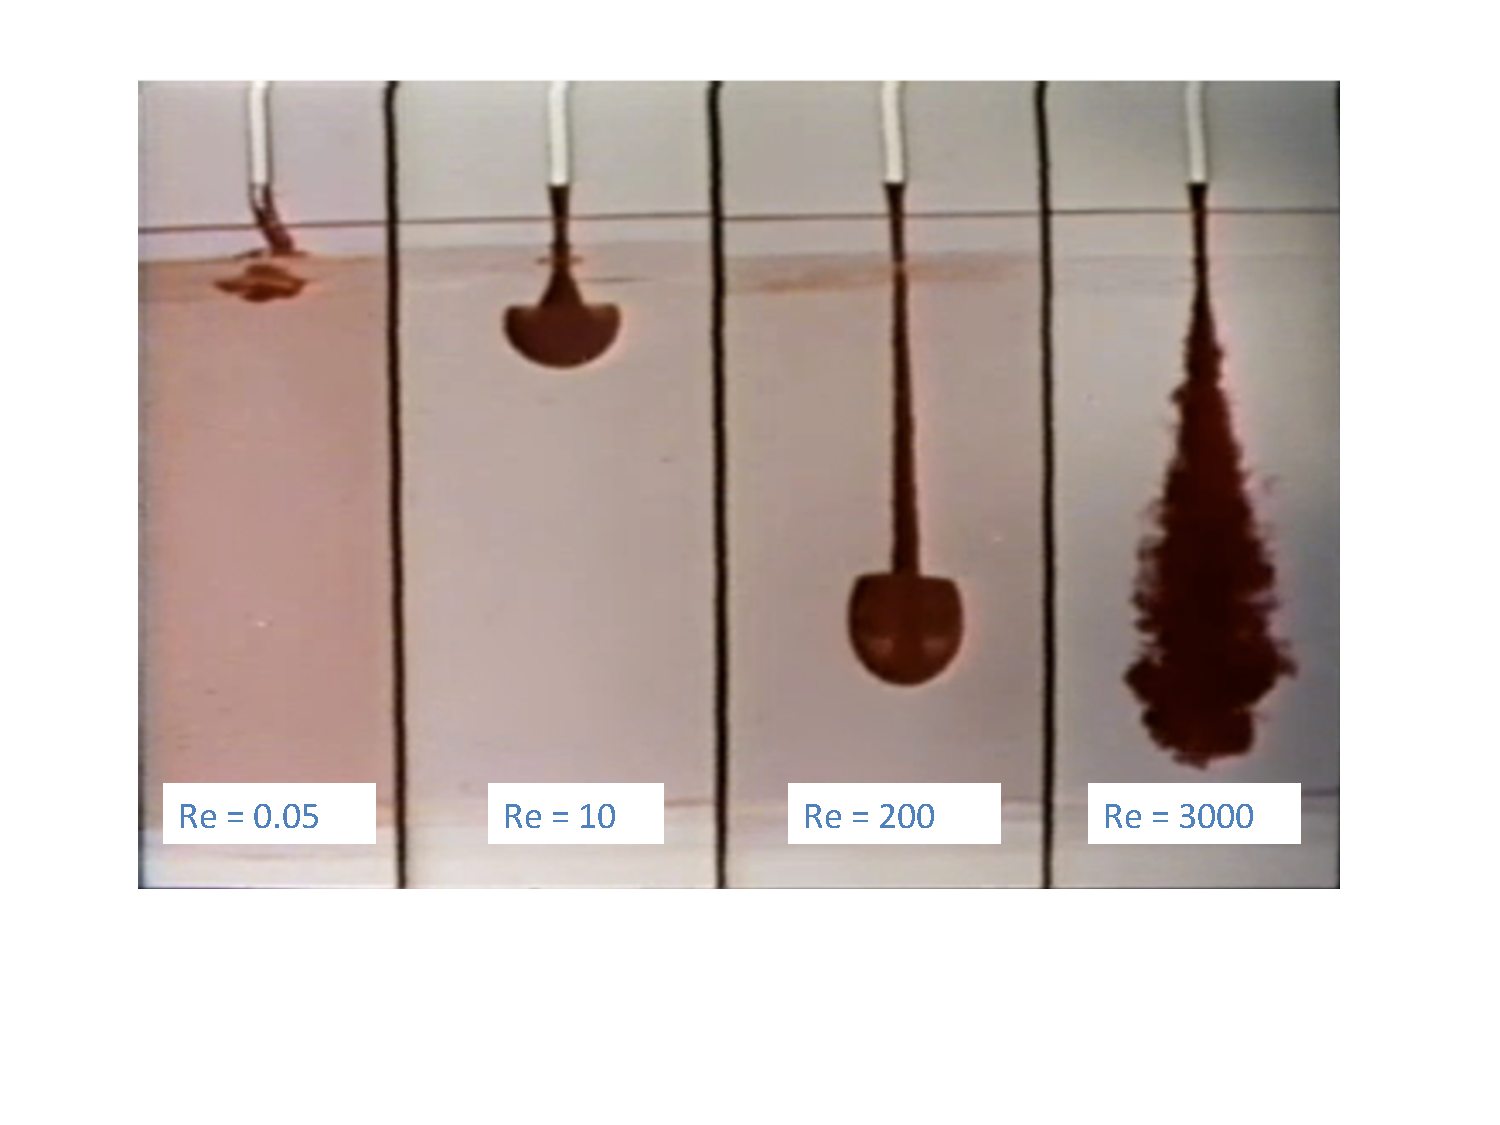
\includegraphics[width=\linewidth]{reynoldsnum_nsf}
\caption[Comparison of flows at varying Reynolds numbers]{
\label{fig:reynoldsnum_nsf}
Flows at varying Reynolds number Re. In each panel, a fluid that has been dyed red is injected from the top into the clear fluid on the bottom. The fluids are a glycerin-water mixture, for which the viscosity can be changed by altering the glycerin to water ratio. By changing the viscosity and the injection speed, it is possible to alter the Reynolds number of the injected flow. The frames show how the flow develops as the Reynolds number is varied. This image is a still from the \href{https://www.youtube.com/playlist?list=PL0EC6527BE871ABA3}{National Committee for Fluid Mechanics Film Series}  \citep{taylor64a}, which, once you get past the distinctly 1960s production values, are a wonderful resource for everything related to fluids.
}
\end{figure}

\section{Modeling Turbulence}

We have remarkably little understanding of how turbulence actually works. However, we have developed some simple models and tools to describe it, and we will next explore those.

\subsection{Velocity Statistics}

One quantity of interest in a turbulent medium is the structure of the velocity field. How does the velocity change from point to point?  In a turbulent medium velocity fluctuates in time and space, and so the best way to proceed is to study those fluctuations statistically. Many statistical tools exist to characterize turbulent motions, and many are used in astrophysics, but we will stick to a few of the simpler ones. We will also make two simplifying assumptions. First we assume that the turbulence is homogenous, in the sense that the turbulent motions vary randomly but not systematically, with position in the fluid. Second, we assume that it is isotropic, so that turbulent motions do not have a preferred directions. Neither of these are likely to be strictly true in a molecular cloud, particularly the second, since large-scale magnetic fields provide a preferred direction, but we will start with these assumptions and relax them later.

Let $\mathbf{v}(\mathbf{x})$ be the velocity at position $\mathbf{x}$ within some volume of interest $V$. To characterize how this varies with position, we define the autocorrelation function
\begin{equation}
A(\mathbf{r})\equiv \frac{1}{V} \int \mathbf{v}(\mathbf{x})\cdot \mathbf{v}(\mathbf{x}+\mathbf{r}) \, d\mathbf{x} \equiv \langle \vecv(\vecx) \cdot \vecv(\vecx+\vecr)\rangle,
\end{equation}
where the angle brackets indicate an average over all positions $\mathbf{x}$. Here, $A(0) = \langle|\vecv|^2\rangle$ is just the mean square velocity in the fluid. If the velocity field is isotropic, then clearly $A(\mathbf{r})$ cannot depend on the direction, and thus must depend only on $r=|\mathbf{r}|$. Thus $A(r)$ tells us how similar or different the velocities are at points separated by some distance $r$.

It is often more convenient to think about this in Fourier space than in real space, so rather than the autocorrelation function we often instead think about its Fourier transform. We define the Fourier transform of the velocity field in the usual way, i.e.\
\begin{equation}
\tilde{\vecv}(\veck) = \frac{1}{\sqrt{2\pi}}\int \vecv(\vecx) e^{-i\veck\cdot\vecx} \,d\vecx.
\end{equation}
We then define the power spectrum
\begin{equation}
\Psi(\veck) \equiv | \tilde{\vecv}(\veck)|^2.
\end{equation}

Again, for isotropic turbulence, the power spectrum depends only on the magnitude of the wave number, $k=|\veck|$, not its direction, so it is more common to talk about the power per unit radius in $k$-space,
\begin{equation}
P(k) = 4\pi k^2 \Psi(k).
\end{equation}
This is just the total power integrated over some shell from $k$ to $k+dk$ in $k$-space. Note that Parseval's theorem tells us that
\begin{equation}
\int P(k)\, dk = \int | \tilde{\vecv}(\veck)|^2 \, d^3\veck = \int \vecv(\vecx)^2 \, d^3\vecx,
\end{equation}
i.e., the integral of the power spectral density over all wavenumbers is equal to the integral of the square of the velocity over all space, so for a flow with constant density (an incompressible flow) the integral of the power spectrum just tells us how much kinetic energy per unit mass there is in the flow. The Wiener-Khinchin theorem also tells us that $P(\veck)$ is just the Fourier transform of the autocorrelation function,
\begin{equation}
\Psi(\veck) = \frac{1}{(2\pi)^{3/2}} \int A(\vecr) e^{-i\veck\cdot\vecr} \,d\vecr.
\end{equation}

The power spectrum at a wavenumber $k$ then just tells us what fraction of the total power is in motions at that wavenumber, i.e., on that characteristic length scale. The power spectrum is another way of looking at the spatial scaling of turbulence. It tells us how much power there is in turbulent motions as a function of wavenumber $k=2\pi/\lambda$. A power spectrum that peaks at low $k$ means that most of the turbulent power is in large-scale motions, since small $k$ corresponds to large $\lambda$. Conversely, a power spectrum that peaks at high $k$ means that most of the power is in small-scale motions.

The power spectrum also tells us about the how the velocity dispersion will vary when it is measured over a region of some characteristic size. Suppose we consider a volume of size $\ell$, and measure the velocity dispersion $\sigma_v(\ell)$ within it. Further suppose that the power spectrum is described by a power law $P(k)\propto k^{-n}$. The total kinetic energy per unit mass within the region is, up to factors of order unity,
\begin{equation}
\mathrm{KE} \sim \sigma_v(\ell)^2,
\end{equation}
but we can also write the kinetic energy per unit mass in terms of the power spectrum, integrating over those modes that are small enough to fit within the volume under consideration:
\begin{equation}
\mathrm{KE} \sim \int_{2\pi/\ell}^\infty P(k) \, dk \propto \ell^{n-1}.
\end{equation}
It therefore follows immediately that
\begin{equation}
\label{eq:vdisp}
\sigma_v = c_s \left(\frac{\ell}{\ell_s}\right)^{(n-1)/2},
\end{equation}
where we have normalized the relationship by defining the sonic scale $\ell_s$ as the size of a region within which the velocity dispersion is equal to the thermal sound speed of the gas.

\subsection{The Kolmogorov Model and Turbulent Cascades}

The closest thing we have to a model of turbulence is in the case of subsonic, hydrodynamic turbulence; the basic theory for that goes back to \citet{kolmogorov41a}.\footnote{An English translation of \citet{kolmogorov41a} (which is in Russian) can be found in \citet{kolmogorov91a}.} Real interstellar clouds are neither subsonic nor hydrodynamic (since they are strongly magnetized, as we discuss in Chapter \ref{ch:magnetic})), but this theory is still useful for understanding how turbulence works. Kolmogorov's theory of turbulence begins with the realization that turbulence is a phenomenon that occurs when Re is large, so that there is a large range of scales where dissipation is unimportant. It is possible to show by Fourier transforming Equation (\ref{eq:momentum}) that for incompressible motion transfer of energy can only occur between adjacent wavenumbers. Energy at a length scale $k$ cannot be transferred directly to some scale $k' \ll k$. Instead, it must cascade through intermediate scales between $k$ and $k'$.

This gives a simple picture of how energy dissipates in fluids. Energy is injected into a system on some large scale that is dissipationless, and it cascades down to smaller scales until it reaches a small enough scale that $\mbox{Re}\sim 1$, at which point dissipation becomes significant. In this picture, if the turbulence is in statistical equilibrium, such that is neither getting stronger or weaker, the energy at some scale $k$ should depend only on $k$ and on the rate of injection or dissipation (which are equal) $\psi$.

This allows us to make the following clever dimensional argument: $k$ has units of $1/L$, i.e., one over length. The power spectrum $P(k)$ has units of energy per unit mass per unit radius in $k$-space. The energy per unit mass is like a velocity squared, so it has units $L^2/T^2$, and this is divided by $k$, so $P(k)$ has units of $L^3/T^2$. The injection and dissipation rates $\psi$ have units of energy per unit mass per unit time, which is a velocity squared divided by a time, or $L^2/T^3$.

Since $P(k)$ is a function only of $k$ and $\psi$, we can write $P(k) = C k^\alpha \psi^\beta$ for some dimensionless constant $C$. Then by dimensional analysis we have
\begin{eqnarray}
\frac{L^3}{T^2} & \sim & L^{-\alpha} \left(\frac{L^2}{T^3}\right)^\beta \\
L^3 & \sim & L^{-\alpha+2\beta} \\
T^{-2} & \sim & T^{-3\beta}\\
\beta & = & \frac{2}{3} \\
\alpha & = & 2\beta - 3 = -\frac{5}{3}
\end{eqnarray}

This immediately tell us three critical things. First, the power in the flow varies with energy injection rate to the $2/3$ power. Second, this power is distributed such that the power at a given wavenumber $k$ varies as $k^{-5/3}$. This means that most of the power is in the largest scale motions, since power diminishes as $k$ increases. Third, if we now take this spectral slope and use it to derive the scale-dependent velocity dispersion from equation (\ref{eq:vdisp}), we find that $\sigma_v \propto \ell^{1/3}$, i.e., velocity dispersion increase with size scale as size to the $1/3$ power. This is an example of what is known in observational astronomy as a linewidth-size relation -- linewidth because the observational diagnostic we use to characterize velocity dispersion is the width of a line. This relationship tells us that larger regions should have larger linewidths, with the linewidth scaling as the 1/3 power of size in the subsonic regime.

The subsonic regime can be tested experimentally on Earth, and Kolmogorov's model provides an excellent fit to observations. Figure \ref{fig:kolmogorov} shows one example.

\begin{figure}
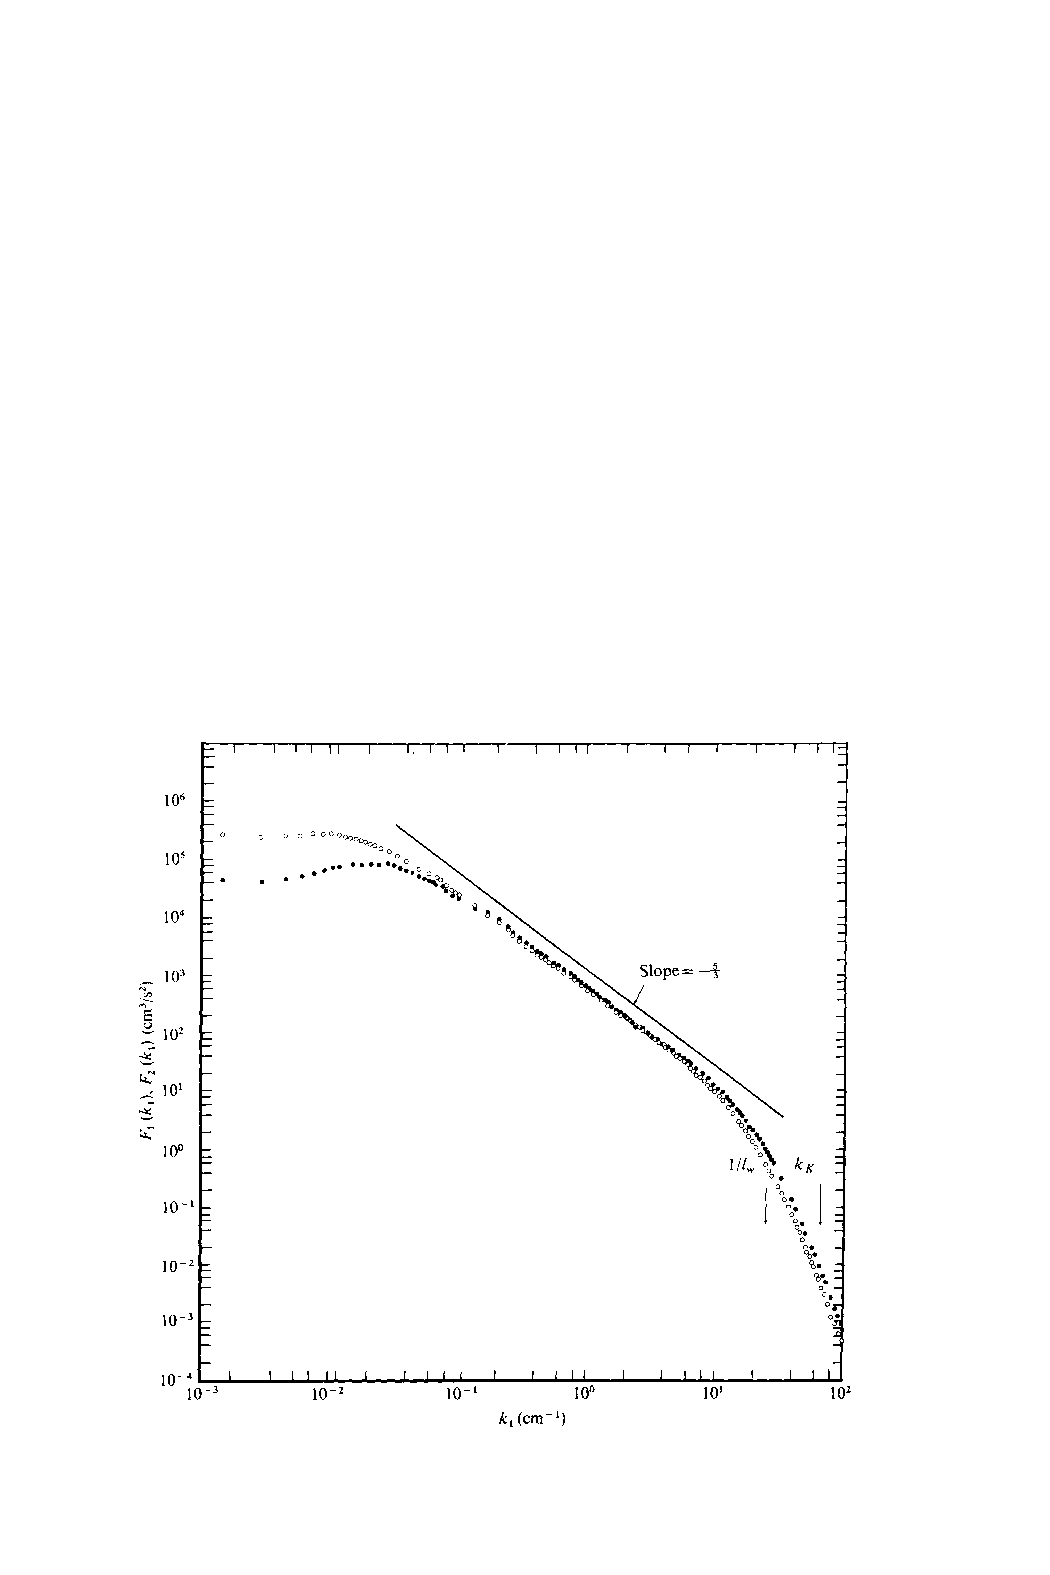
\includegraphics[width=\linewidth]{kolmogorov_champagne78}
\caption[Experimental power spectra for Kolmogorov turbulence]{
\label{fig:kolmogorov}
An experimentally-measured power spectrum for turbulence generated by an air jet \citep{champagne78a}. The $x$ axis is the wavenumber, and the open and filled points show the velocity power spectrum for the velocity components parallel and transverse to the stream, respectively.
}
\end{figure}

\section{Supersonic Turbulence}

\subsection{Velocity Statistics}

We have seen that real interstellar clouds not only have $\mathrm{Re} \gg 1$, they also have $\mathcal{M} \gg 1$, and so the flows within them are supersonic. This means that pressure is unimportant on size scales $L \gg \ell_s$. Since viscosity is also unimportant on large scales (since $\mbox{Re} \gg 1$), this means that gas tends to move ballistically on large scales. On small scales this will produce very sharp gradients in velocity, since fast-moving volumes of fluid will simply overtake slower ones. Since the viscosity term gets more important on smaller scales, the viscosity term will eventually stop the fluid from moving ballistically. In practice this means the formation of shocks -- regions where the flow velocity changes very rapidly, on a size scale determined by the viscosity.\footnote{In real interstellar clouds the relevant viscosity is the magnetic one, as we shall see in Chapter \ref{ch:magnetic}.}

We expect that the velocity field that results in this case will look like a series of step functions. The power spectrum of a step function is a power law $P(k)\propto k^{-2}$. One can establish this easily from direct calculation. Let us zoom in on the region around a shock, so that the change in velocity on either side of the shock is small. The Fourier transform of $v$ in 1D is
\begin{equation}
\tilde{v}(k) = \frac{1}{\sqrt{2\pi}} \int v(x) e^{-i kx}\, dx
\end{equation}
The integral of the periodic function $e^{-ikx}$ vanishes for all periods in the regions where $v$ is constant. It is non-zero only in the period that includes the shock. The amplitude of $\int v(x) e^{-i kx}\, dx$ during that period is simply proportional to the length of the period, i.e., to $1/k$. Thus, $\tilde{v}(k)\propto 1/k$. It then follows that $P(k)\propto k^{-2}$ for a single shock. An isotropic system of overlapping shocks should therefore also look approximately like a power law of similar slope. This gives a velocity dispersion versus size scale $\sigma_v\propto \ell^{1/2}$, and this is exactly what is observed. Figure \ref{fig:polaris} shows an example.

\begin{marginfigure}
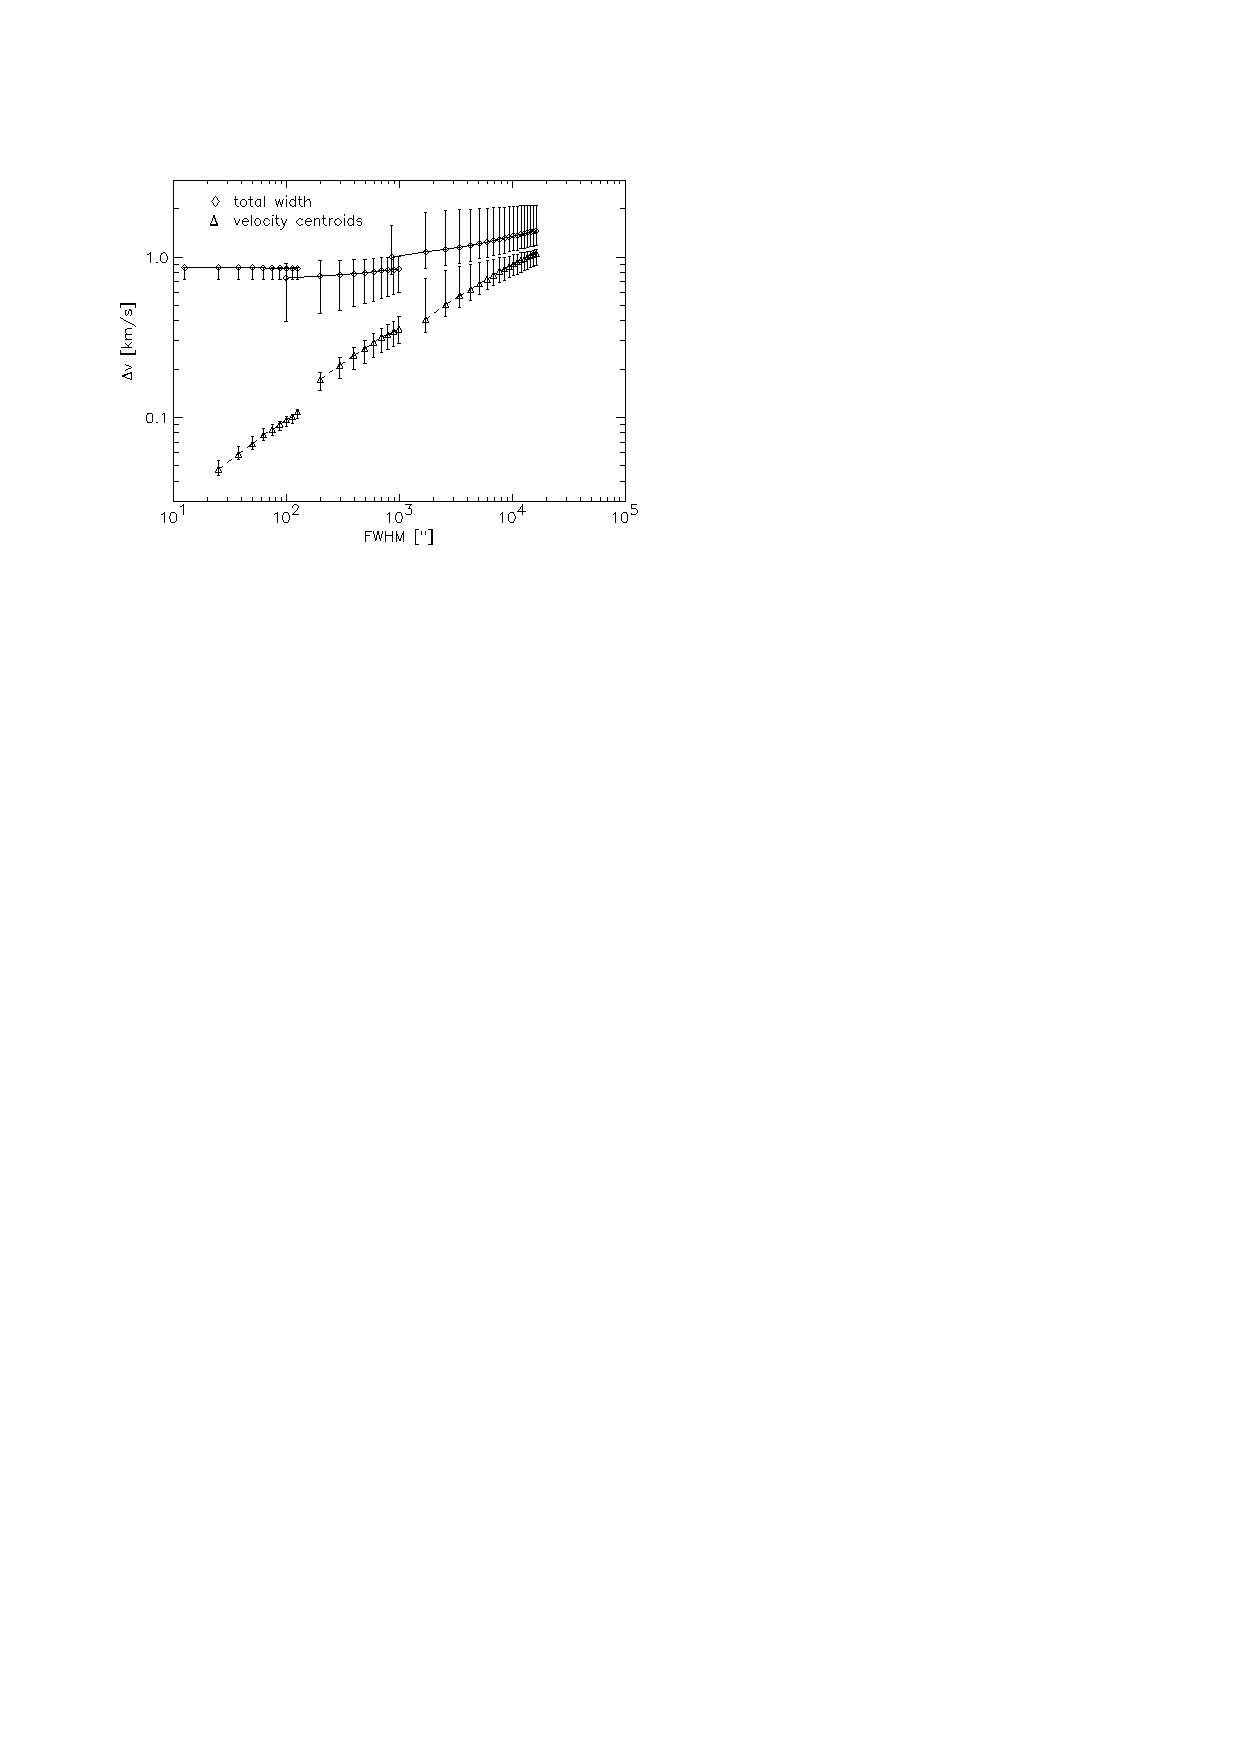
\includegraphics[width=\linewidth]{polaris_ossenkopf02}
\caption[Linewidth versus size in the Polaris Flare cloud]{
\label{fig:polaris}
Linewidth versus size in the Polaris Flare Cloud obtained from CO observations \citep{ossenkopf02a}. Diamonds show the total measured velocity width within apertures of the size indicated on the $x$ axis, while triangles show the dispersion obtained by taking the centroid velocity in each pixel and measuring the dispersion of centroids. The three sets of points joined by lines represent measurements from three separate telescopes.
}
\end{marginfigure}

Note that, although the power spectrum is only slightly different than that of subsonic turbulence ($-2$ versus about $-5/3$), there is really an important fundamental difference between the two regimes. Most basically, in Kolmogorov turbulence decay of energy happens via a cascade from large to small scales, until a dissipative scale is reached. In the supersonic case, on the other hand, the decay of energy is via the formation of shocks, and as we have just seen a single shock generates a power spectrum $\propto k^{-2}$, i.e., it non-locally couples many scales. Thus, in supersonic turbulence there is no locality in $k$-space. All scales are coupled at shocks.

\subsection{Density Statistics}

In subsonic flows the pressure force is dominant. Thus if the gas is isothermal, then the density stays nearly constant -- any density inhomogeneities are ironed out immediately by the strong pressure forces. In supersonic turbulence, on the other hand, the flow is highly compressible. It is therefore of great interest to ask about the statistics of the density field.

Numerical experiments and empirical arguments (but not fully rigorous proofs) indicate that the density field for a supersonically-turbulent, isothermal medium is well-described by a lognormal distribution,
\begin{equation}
\label{eq:denpdf}
p(s) = \frac{1}{\sqrt{2\pi \sigma_s^2}} \exp\left[-\frac{(s-s_0)^2}{2\sigma_s^2}\right],
\end{equation}
where $s=\ln(\rho/\overline{\rho})$ is the log of the density normalized to the mean density $\overline{\rho}$. This distribution describes the probability that the density at a randomly chosen point will be such that $\ln(\rho/\overline{\rho})$ is in the range from $s$ to $s+ds$. The median of the distribution $s_0$ and the dispersion $\sigma_s$ must be related to one another, because we require that
\begin{equation}
\overline{\rho} = \int p(s) \rho \, ds.
\end{equation}
With a bit of algebra, one can show that this equation is satisfied if and only if
\begin{equation}
s_0 = -\sigma_s^2/2.
\end{equation}

Instead of computing the probability that a randomly chosen point in space will have a particular density, we can also compute the probability that a randomly chosen mass element will have a particular density. This more or less amounts to a simple change of variables. Consider some volume of interest $V$, and examine all the material with density such that $\ln(\rho/\overline{\rho})$ is in the range from $s$ to $s+ds$. This material occupies a volume $dV = p(s) V$, and thus must have a mass
\begin{eqnarray}
dM & = & \rho p(s) \, dV \\
& = & \overline{\rho} e^s \cdot \frac{1}{\sqrt{2\pi \sigma_s^2}} \exp\left[-\frac{(s-s_0)^2}{2\sigma_s^2}\right]\,  dV \\
& = & \overline{\rho} \frac{1}{\sqrt{2\pi \sigma_s^2}} \exp\left[-\frac{(s+s_0)^2}{2\sigma_s^2}\right]\,  dV
\end{eqnarray}
It immediately follows that the mass PDF is simply
\begin{equation}
p_M(s) = \frac{1}{\sqrt{2\pi \sigma_s^2}} \exp\left[-\frac{(s+s_0)^2}{2\sigma_s^2}\right],
\end{equation}
i.e., exactly the same as the volume PDF but with the peak moved from $-s_0$ to $+s_0$. Physically, the meaning of these shifts is that the typical volume element in a supersonic turbulent field is at a density lower than the mean, because much of the mass is collected into shocks. The typical mass element lives in one of these shocked regions, and thus is at higher-than-average density. Figure \ref{fig:turbrender} shows an example of the density distribution produced in a numerical simulation of supersonic turbulence.
\begin{marginfigure}
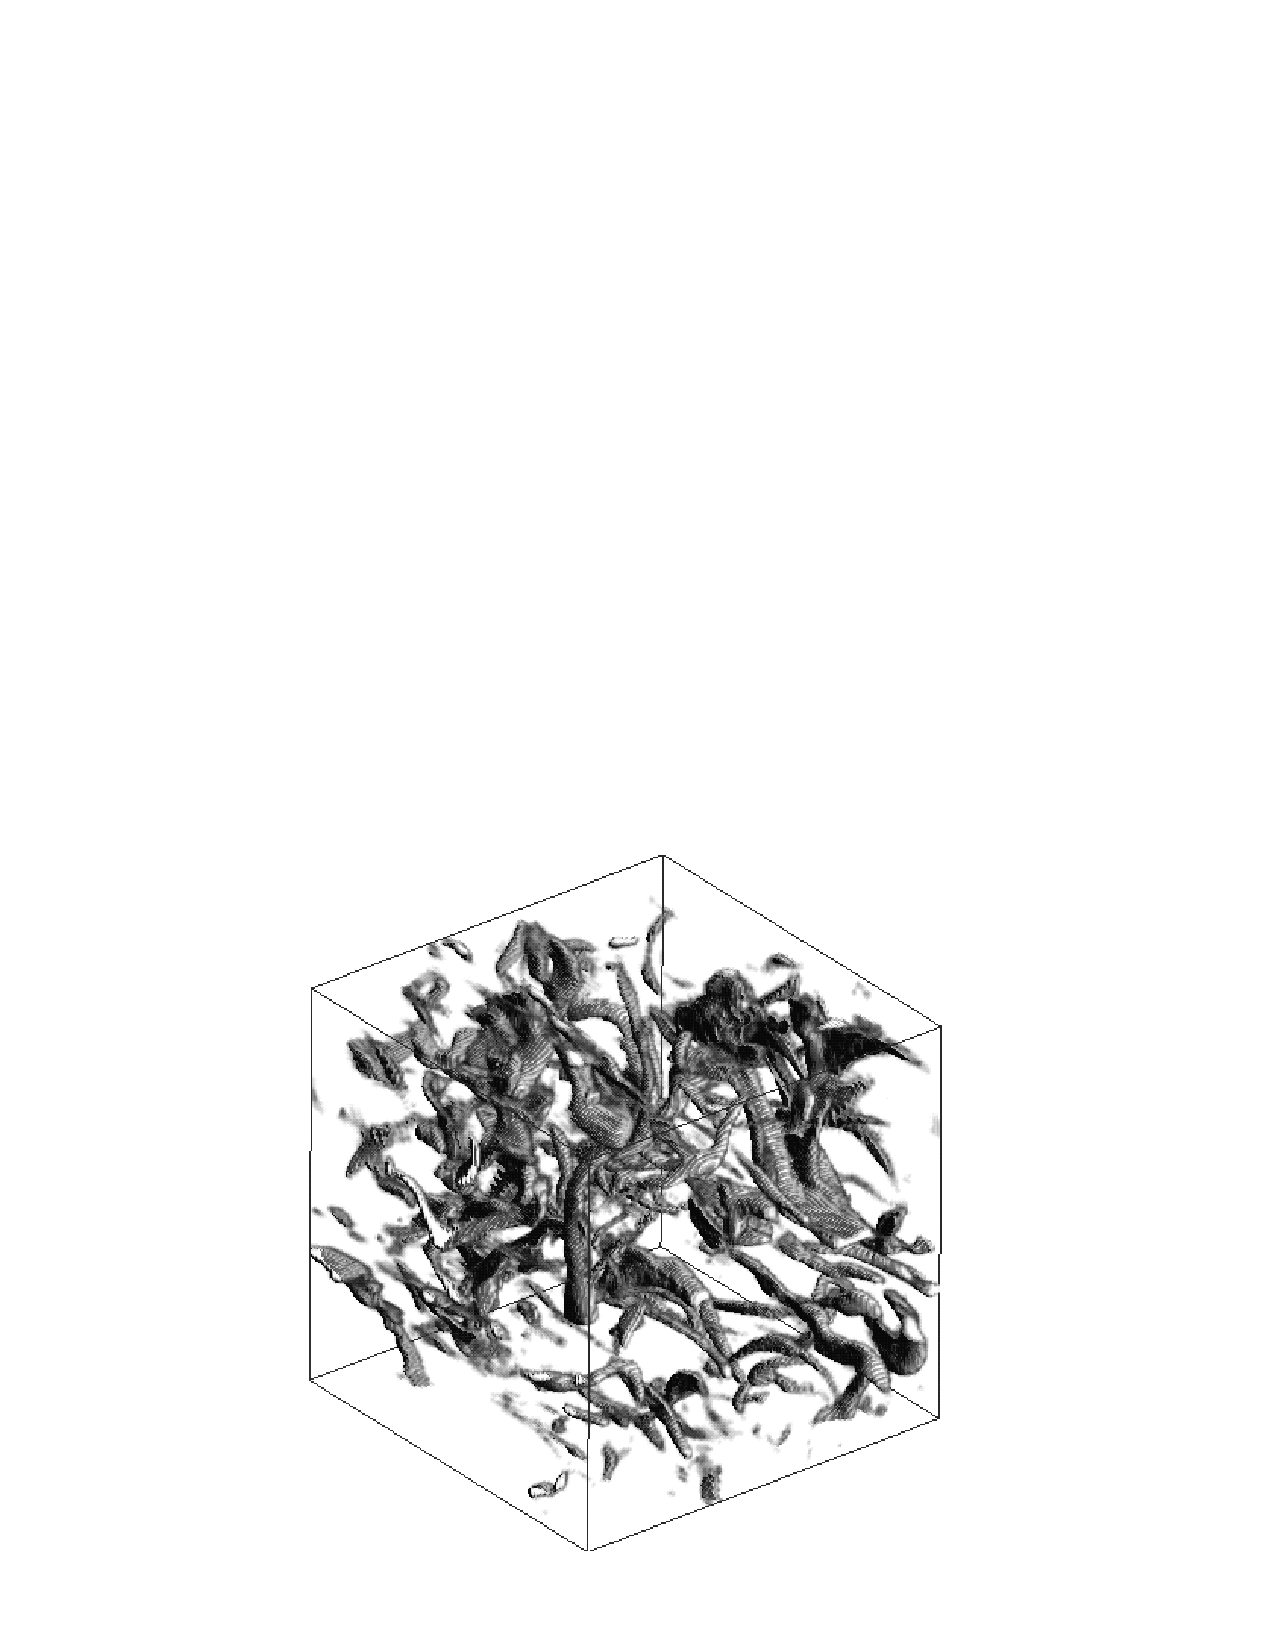
\includegraphics[width=\linewidth]{turbrender_padoan99}
\caption[Volume rendering of the density field for supersonic turbulence]{
\label{fig:turbrender}
Volume rendering of the density field in a simulation of supersonic turbulence \citep{padoan99a}. The surfaces shown are isosurfaces of density.
}
\end{marginfigure}

The lognormal functional form is not too surprising, given the central limit theorem. Supersonic turbulence consists of an alternating series of shocks, which cause the density to be multiplied by some factor, and supersonic rarefactions, which cause it to drop by some factor. The result of multiplying a lot of positive density increases by a lot of negative density drops at random tends to produce a normal distribution in the multiplicative factor, and thus a lognormal distribution in the density.

This argument does not, however, tell us about the dispersion of densities, which must be determined empirically from numerical simulations. The general result of these simulations \citep[e.g.,][]{federrath13b} is that
\begin{equation}
\sigma_s^2 \approx \ln \left(1 + b^2 \mathcal{M}^2 \frac{\beta_0}{\beta_0+1}\right),
\end{equation}
where the factor $b$ is a number in the range $1/3-1$ that depends on how compressive versus solenoidal the velocity field is, and $\beta_0$ is the ratio of thermal to magnetic pressure at the mean density and magnetic field strength, something we will discuss further in Chapter \ref{ch:magnetic}.

In addition to the density PDF, there are higher order statistics describing correlations of the density field from point to point. We will defer a discussion of these until we get to models of the IMF in Chapter \ref{ch:imf_th}, where they play a major role.



%------------------------------------------------

%\section{Section 1 - Fullwidth Environment Example}

%\begin{fullwidth}
%\lipsum[5]
%\end{fullwidth}

%\subsection{Subsection 1}

%\lipsum[6-7]

%\subsection{Subsection 2}

%\lipsum[7-8]

%------------------------------------------------

%\section{Section 2}

%\subsection{Subsection 1}

%\lipsum[9-10]

%\subsection{Subsection 2}

%\lipsum[11-12]

%----------------------------------------------------------------------------------------
%	CHAPTER 2
%----------------------------------------------------------------------------------------

%\chapter{Chapter 2 Title}
%\label{ch:2}

%\lipsum[13-20]

%----------------------------------------------------------------------------------------

\backmatter

%----------------------------------------------------------------------------------------
%	BIBLIOGRAPHY
%----------------------------------------------------------------------------------------

\bibliography{bib/refs} % Use the bibliography.bib file for the bibliography
%\bibliographystyle{plainnat} % Use the plainnat style of referencing
\bibliographystyle{apj}

%----------------------------------------------------------------------------------------

\printindex % Print the index at the very end of the document

\end{document}